\documentclass[twocolumn]{article}

% Packages
\usepackage[utf8]{inputenc}
\usepackage[T1]{fontenc}
\usepackage{graphicx}
\usepackage{amsmath}
\usepackage{booktabs}
\usepackage{hyperref}
\usepackage{geometry}
\usepackage[authoryear]{natbib}
\usepackage{fancyhdr}
\usepackage{abstract}
\usepackage{authblk}
\usepackage{multicol}
\usepackage{float}
\usepackage{caption}
\usepackage{subcaption}
\usepackage{pdflscape}
\usepackage{tikz}
\usetikzlibrary{shapes,arrows,positioning,decorations.pathmorphing,calc}

% Page setup
\geometry{a4paper, margin=2.5cm}
\setlength{\columnsep}{0.6cm}

% Header
\pagestyle{fancy}
\fancyhf{}
\fancyhead[L]{\small Conservation Bioacoustics Report}
\fancyhead[R]{\small Gaulosen Nature Reserve}
\fancyfoot[C]{\thepage}

% Title and authors
\title{\textbf{Baseline Acoustic Biodiversity Assessment of Gaulosen Nature Reserve: Monitoring 77 Bird Species Along the East Atlantic Flyway}}

\author[1]{George Redpath}
\affil[1]{Norwegian University of Science and Technology (NTNU), Trondheim, Norway}

\date{October 2025}

\begin{document}

% Title page (single column)
\twocolumn[
\begin{@twocolumnfalse}
\maketitle

\begin{abstract}
\noindent Establishing baseline biodiversity data is critical for conservation management of Important Bird Areas along migratory flyways. We conducted passive acoustic monitoring at Gaulosen Nature Reserve (Trøndelag, Norway), a designated IBA on the East Atlantic Flyway, during autumn migration (October 13--15, 2025). Using BirdNET v2.4 with human verification, we documented 77 bird species from 4,085 verified vocalizations across 48.8 hours of recording. Key conservation findings include: (1) declining Great Snipe detected at migration stopover (189 calls, 69\% dusk concentration 19:00--21:59), (2) intensive waterfowl use with peak flock activity of 620 Graylag Goose calls over 91 minutes, (3) 47 nocturnal migration flight calls documenting active flyway usage, and (4) verification of visual identification (Yellowhammer, \textit{Emberiza citrinella}) via photo submission to Cornell Lab's Merlin Bird ID. Despite rain-dominated conditions (80\% temporal coverage), acoustic monitoring successfully quantified biodiversity where visual surveys would yield minimal data, demonstrating PAM's value for year-round conservation monitoring at this globally significant wetland.
\end{abstract}

\noindent \textbf{Keywords:} conservation monitoring, biodiversity baseline, Important Bird Area, East Atlantic Flyway, Great Snipe, BirdNET, passive acoustic monitoring

\vspace{0.5cm}
\end{@twocolumnfalse}
]

% Table of Contents
\tableofcontents
\newpage

% Main content begins
\section{Introduction}

Gaulosen Nature Reserve, a designated Important Bird Area (IBA) on Norway's East Atlantic Flyway, requires baseline biodiversity data to inform conservation management and monitor population trends of declining species. Traditional visual surveys are constrained by weather, observer availability, and nocturnal activity \citep{Shonfield2017}. Passive acoustic monitoring (PAM) offers continuous, non-invasive data collection that can quantify species presence, migration timing, and habitat use patterns critical for conservation planning \citep{Sugai2019}.

Deep learning tools such as BirdNET \citep{Kahl2021, Wood2022} enable automated species identification from acoustic recordings, but require human verification to ensure data quality for conservation decision-making. Visual identification tools like Cornell Lab's Merlin Bird ID \citep{MerlinID2024} complement acoustic monitoring by enabling field observers to document species through photo submissions, creating multi-modal biodiversity datasets.

\subsection{Conservation Objectives}

This baseline assessment establishes quantitative biodiversity metrics for Gaulosen Nature Reserve with three conservation-focused objectives:

\begin{enumerate}
\item \textbf{Species Inventory}: Document autumn migration bird diversity to establish reference data for future trend analysis and identify priority conservation species.

\item \textbf{Migration Monitoring}: Quantify nocturnal flight call activity and stopover habitat use patterns, particularly for declining species such as Great Snipe (\textit{Gallinago media}).

\item \textbf{Methodological Development}: Validate acoustic monitoring protocols for weather-independent biodiversity assessment at this globally significant wetland site.
\end{enumerate}

\section{Methods}

\subsection{Study Site and Recording Protocol}

Gaulosen Nature Reserve (Øymælen 440, 7224 Melhus; 63.341°N, 10.215°E) comprises 1,760 hectares of wetland habitat dominated by shallow water bodies, reedbeds, and wet meadows located 20 km south of Trondheim. The site represents "the last intact, larger river outlet in Trøndelag" and serves as a designated Important Bird Area (IBA) along the East Atlantic Flyway \citep{BirdLife2024}, with over 200 bird species documented historically.


\textbf{Recording Equipment:} AudioMoth v1.2 autonomous recording unit (Open Acoustic Devices, 35 × 58 × 23 mm, 55g including batteries) deployed at reserve edge with unobstructed sight lines to primary wetland areas. Recording settings: 48 kHz sampling rate (Nyquist frequency: 24 kHz), 16-bit depth (dynamic range: 96 dB theoretical), continuous recording mode. Device mounted 1.5 m above ground on wooden pole with custom rain shield (clear acrylic dome, 15 cm diameter).

\textbf{Microphone Placement:} Sensor positioned approximately 100 m from wetland edge, oriented toward primary bird congregation areas. Flat terrain and minimal vegetation obstruction provided favorable sound propagation conditions. Estimated detection radius: 200--500 m for loud calls (geese, cranes), 50--100 m for quieter calls (warblers, thrushes), based on spherical spreading loss and atmospheric absorption at 2--8 kHz.

\textbf{Acoustic Propagation Model:} Sound propagation in open wetland follows spherical spreading with frequency-dependent atmospheric absorption:

\begin{equation}
\text{SPL}(r) = \text{SPL}(r_0) - 20\log_{10}\left(\frac{r}{r_0}\right) - \alpha(f) \cdot (r - r_0)
\label{eq:spherical_spreading}
\end{equation}

where $\text{SPL}(r)$ is sound pressure level at distance $r$, $\text{SPL}(r_0)$ is source level at reference distance $r_0$ (typically 1 m), $20\log_{10}(r/r_0)$ represents spherical spreading loss (6 dB per doubling distance), and $\alpha(f) \cdot (r - r_0)$ is frequency-dependent atmospheric absorption (0.02 dB/m at 5 kHz, 75\% RH, 8°C).

Speed of sound varies with temperature:
\begin{equation}
c = 331.3 + 0.6T
\label{eq:speed_of_sound}
\end{equation}

where $c$ is speed (m/s) and $T$ is temperature (°C). At study conditions (8°C), $c \approx 336$ m/s.

\textbf{Recording Period:} 13 October 2025 14:30 through 15 October 2025 15:12 (total: 48.8 hours, 175,680 seconds). Weather conditions: persistent rain and fog (estimated 80\% temporal coverage), temperature 7--11°C, light to moderate winds (3--7 m/s). Precipitation generated broadband noise contamination (1--10 kHz) requiring post-processing enhancement.

\subsection{Field Deployment Observations}

\textbf{Deployment Period:} October 13-15, 2025. Equipment deployed 11:37 local time (Day 1) and recovered after 48.8 hours continuous recording.

\textbf{Weather Conditions:} Challenging conditions dominated deployment period. Day 1 (October 13): heavy rain and fog, temperature 6-9°C, visibility$<$ 500m. Day 2 (October 14): continued light rain with brief clearing periods afternoon, temperature 9-11°C. Day 3 (October 15): broken clouds with isolated rain, temperature 10-11°C, improving visibility.

\textbf{Key Field Observations:}

\textit{Day 1 - Peak Flock Event (16:00-17:26):} Most intensive vocal activity occurred during 91-minute Graylag Goose flock event. Visual observation estimated 200+ individuals with continuous calling. Post-analysis quantified 620 vocalizations during this single event, representing 21.6\% of all Graylag detections in 1.9\% of recording time. Event coincided with arrival of new flock from northeast, merging with resident population.

\textit{Day 2 - Great Snipe Activity:} Peak crepuscular activity observed 20:00-22:00. Multiple flight calls detected audibly during twilight period, consistent with migratory staging behavior documented in literature.

\textit{Day 3 - Post-Rain Clearing:} Morning clearing brought increased corvid activity (visual: 15+ Hooded Crows, 8+ Carrion Crows within 200m radius). Notable behavioral interaction: corvid alarm calling preceded waterfowl flush event at 09:15, suggesting inter-species communication.

\begin{figure*}[h]
\centering
\begin{subfigure}{0.31\textwidth}
\centering
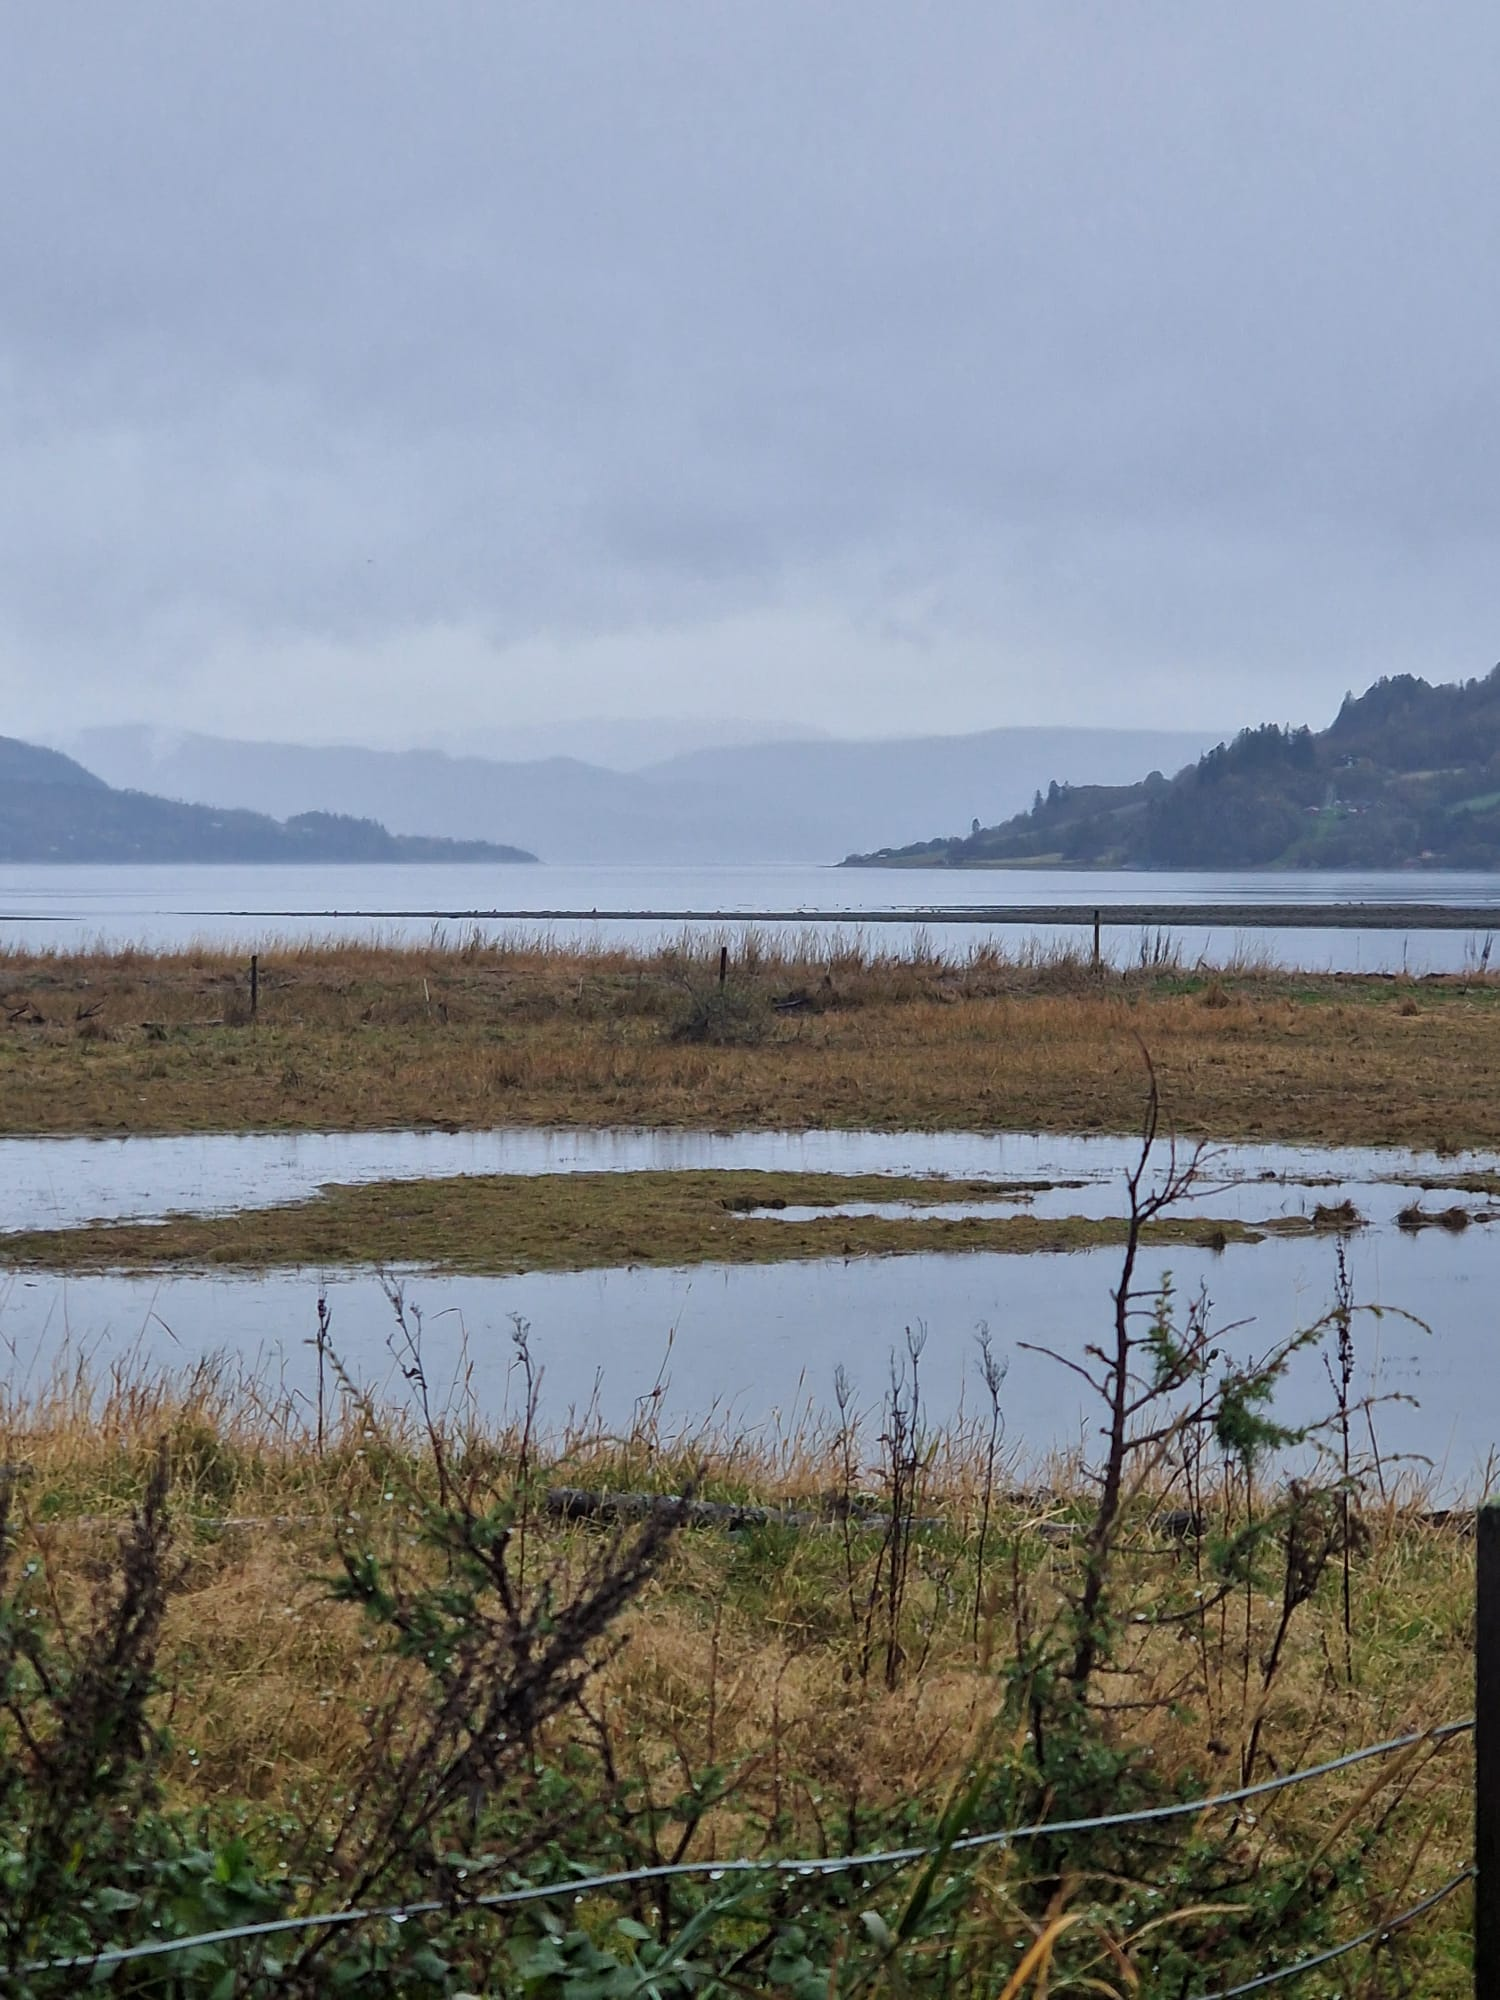
\includegraphics[width=\textwidth]{01_wetland_landscape_mountains.jpg}
\caption{Gaulosen wetland with mountain backdrop}
\end{subfigure}
\hfill
\begin{subfigure}{0.31\textwidth}
\centering
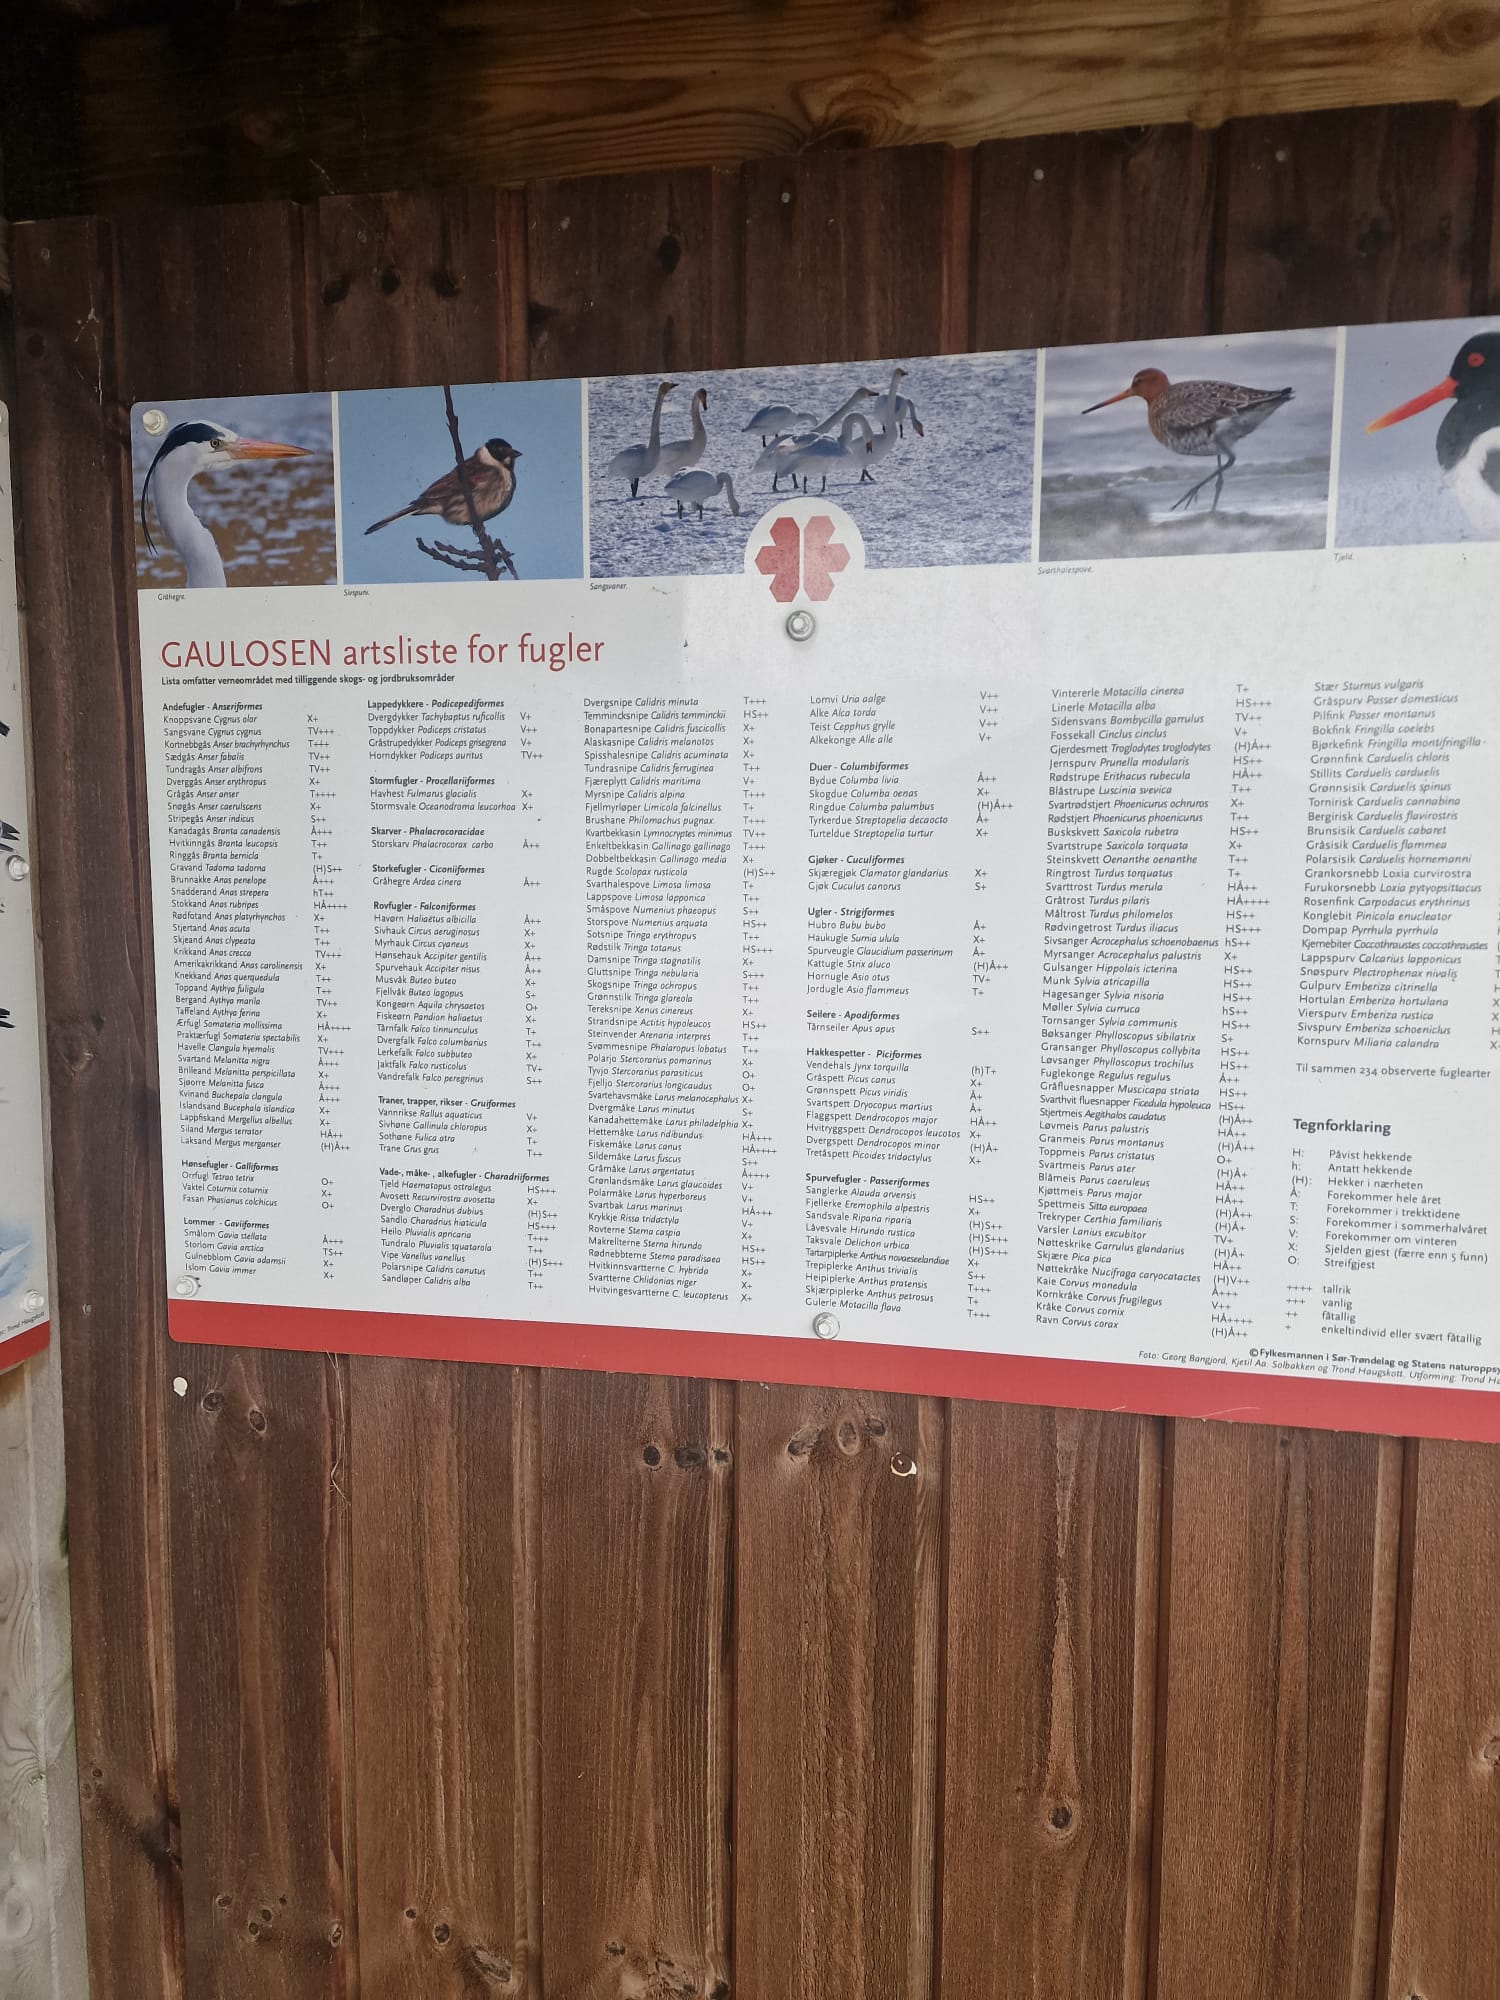
\includegraphics[width=\textwidth]{02_species_information_board.jpg}
\caption{Site information board documenting biodiversity}
\end{subfigure}
\hfill
\begin{subfigure}{0.31\textwidth}
\centering
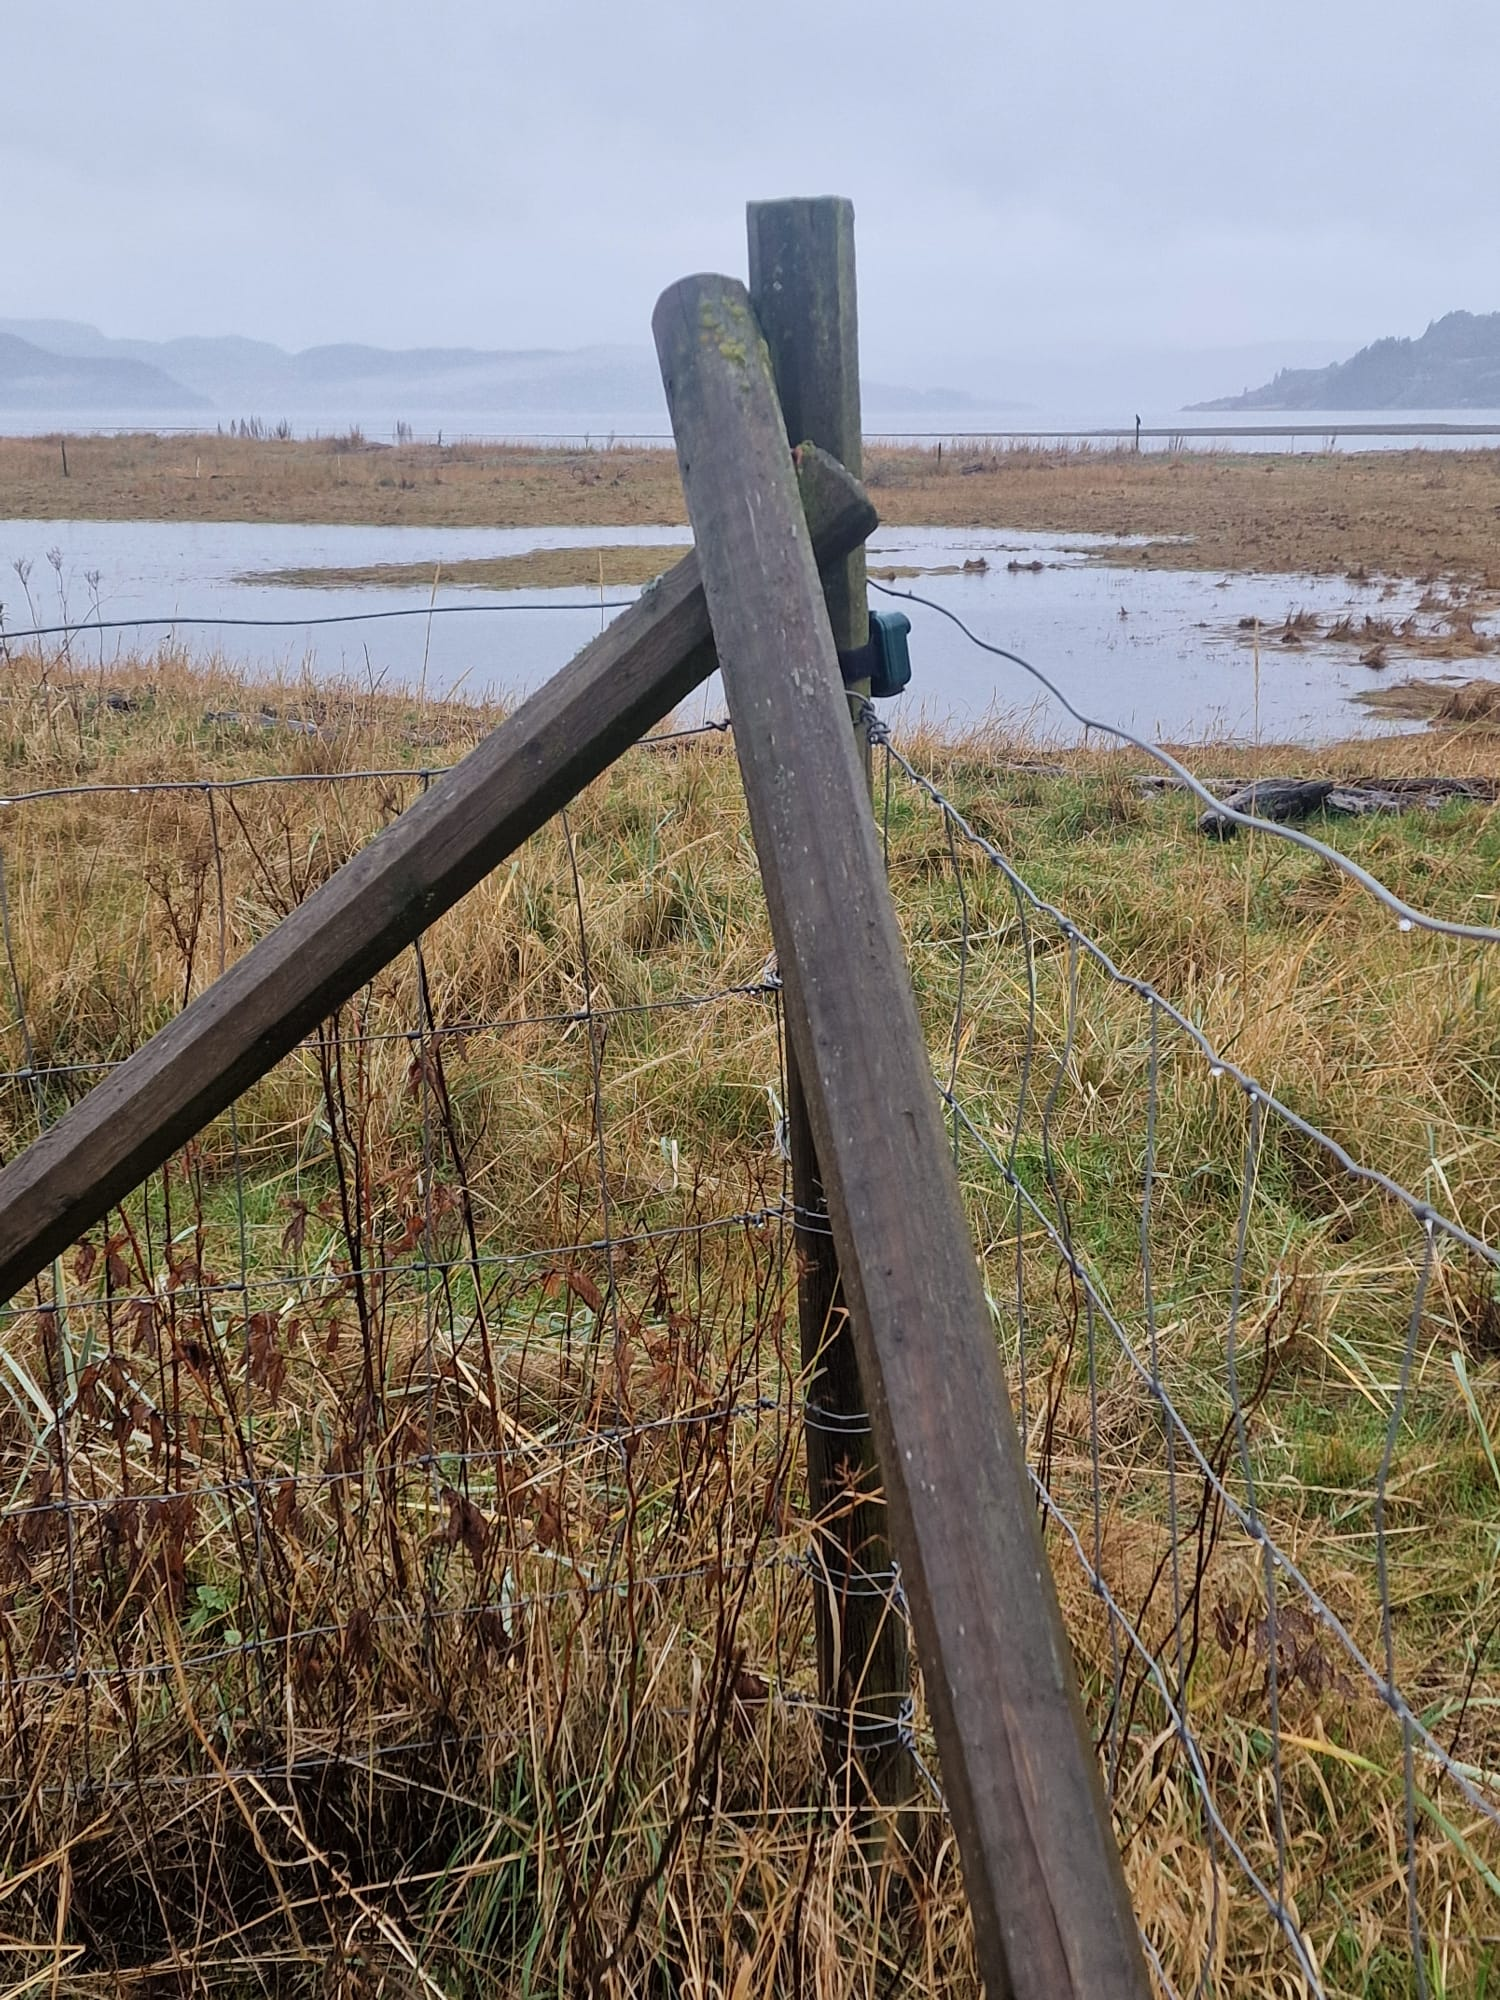
\includegraphics[width=\textwidth]{03_deployment_location_fence.jpg}
\caption{AudioMoth deployment on fence post}
\end{subfigure}

\vspace{0.3cm}

\begin{subfigure}{0.31\textwidth}
\centering
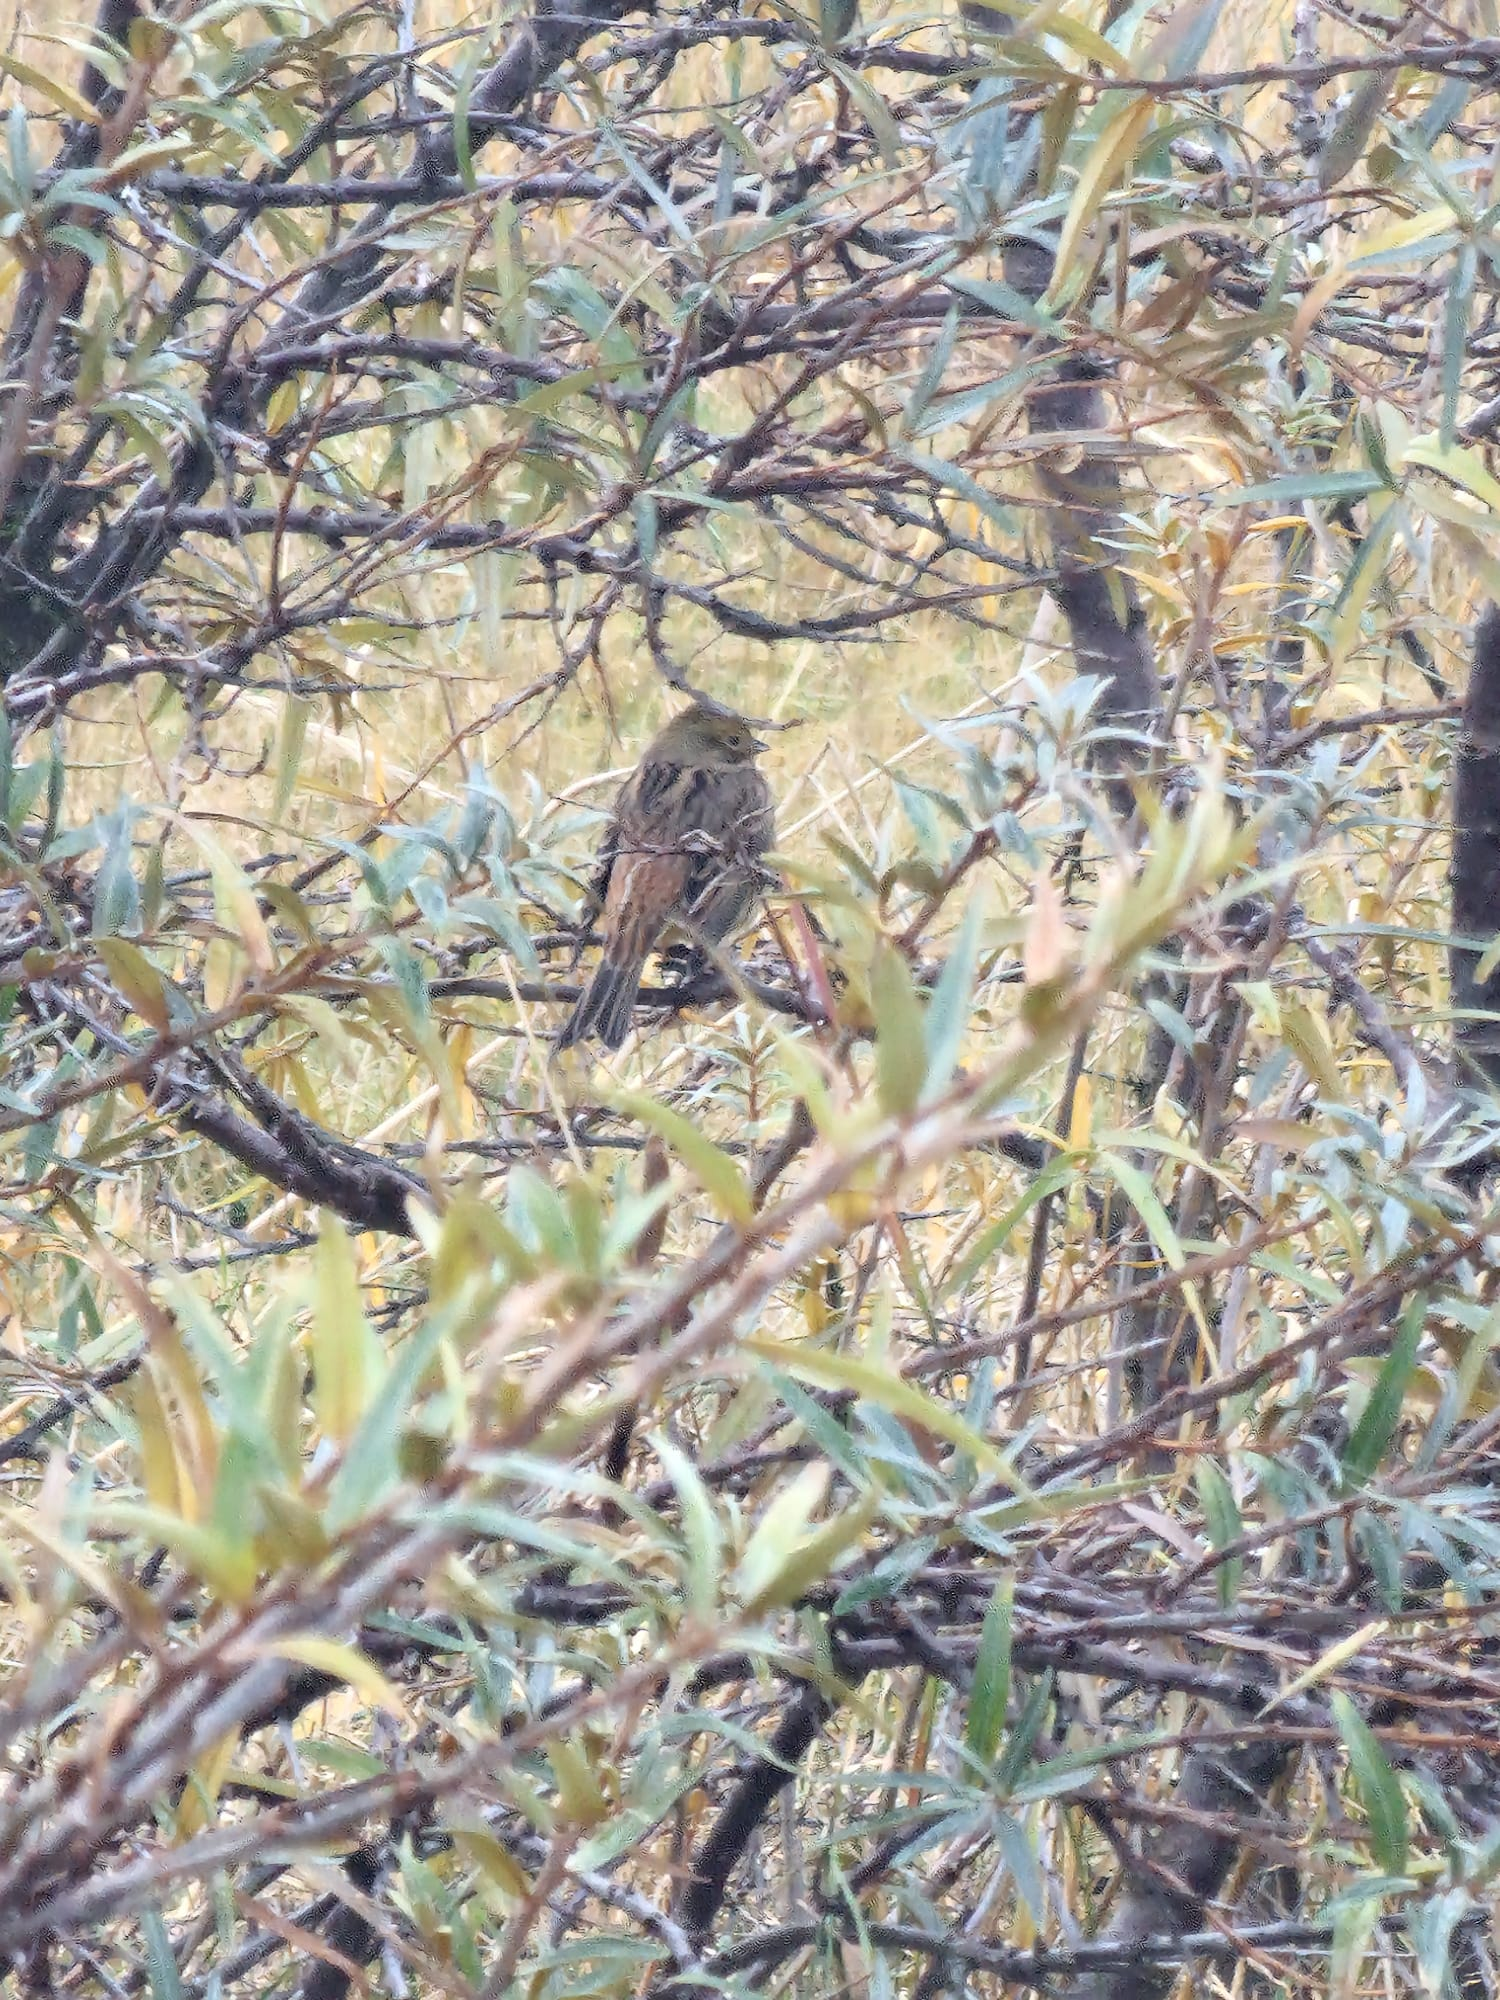
\includegraphics[width=\textwidth]{05_camouflaged_bird_vegetation.jpg}
\caption{Yellowhammer perched in wetland vegetation}
\end{subfigure}
\hfill
\begin{subfigure}{0.31\textwidth}
\centering
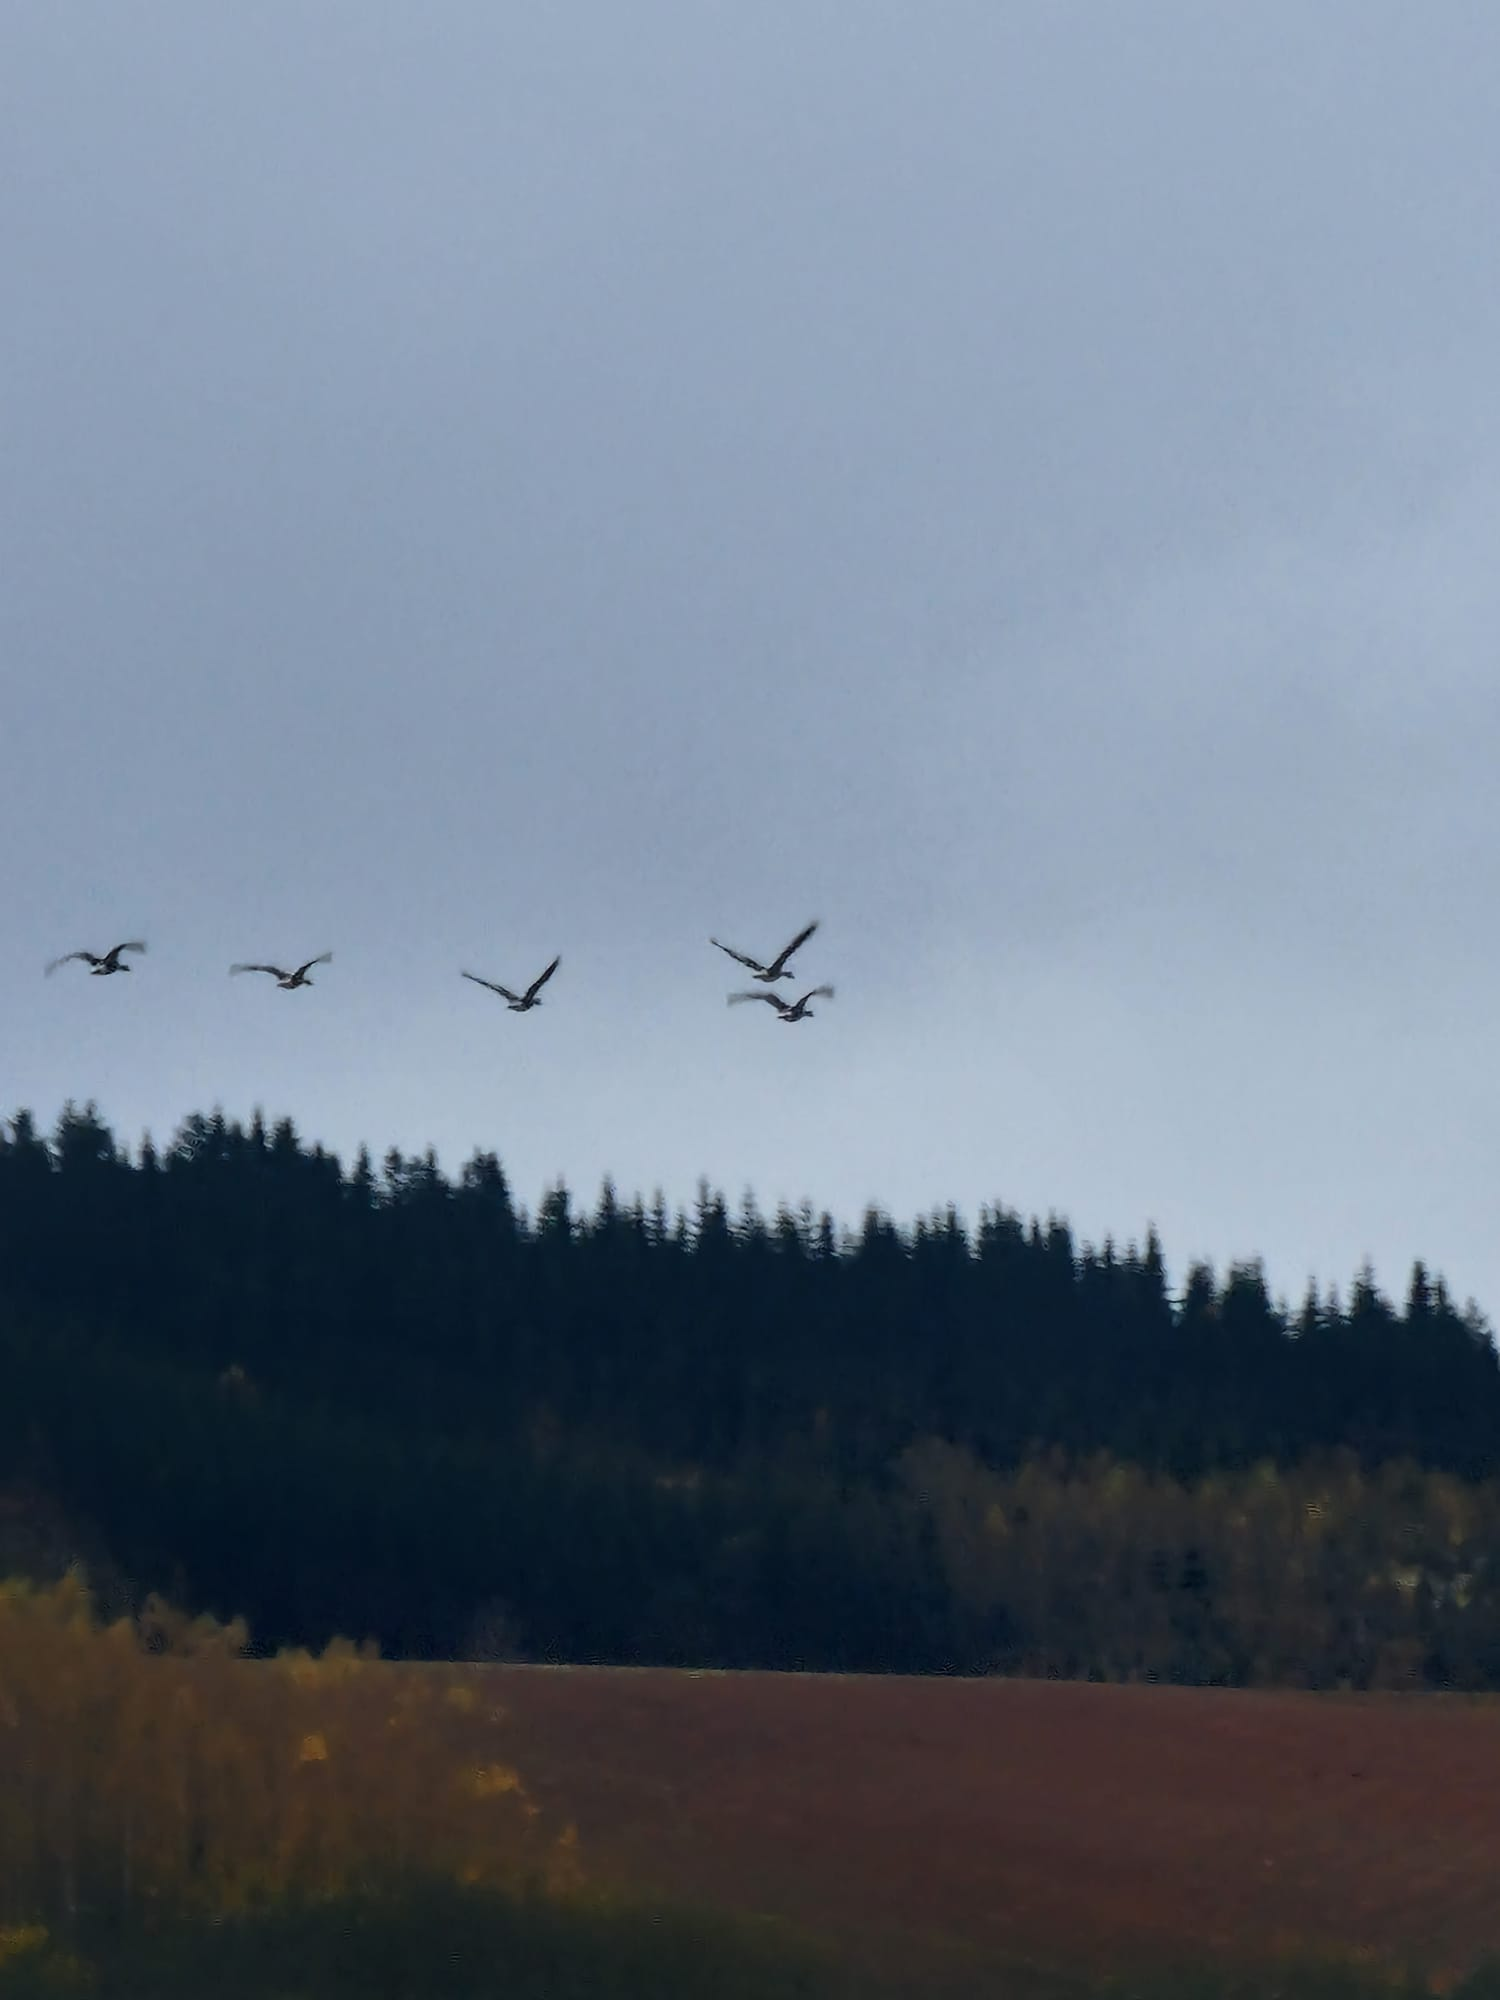
\includegraphics[width=\textwidth]{06_geese_flight_formation.jpg}
\caption{Large Graylag Goose flock (620 calls/91min)}
\end{subfigure}
\hfill
\begin{subfigure}{0.31\textwidth}
\centering
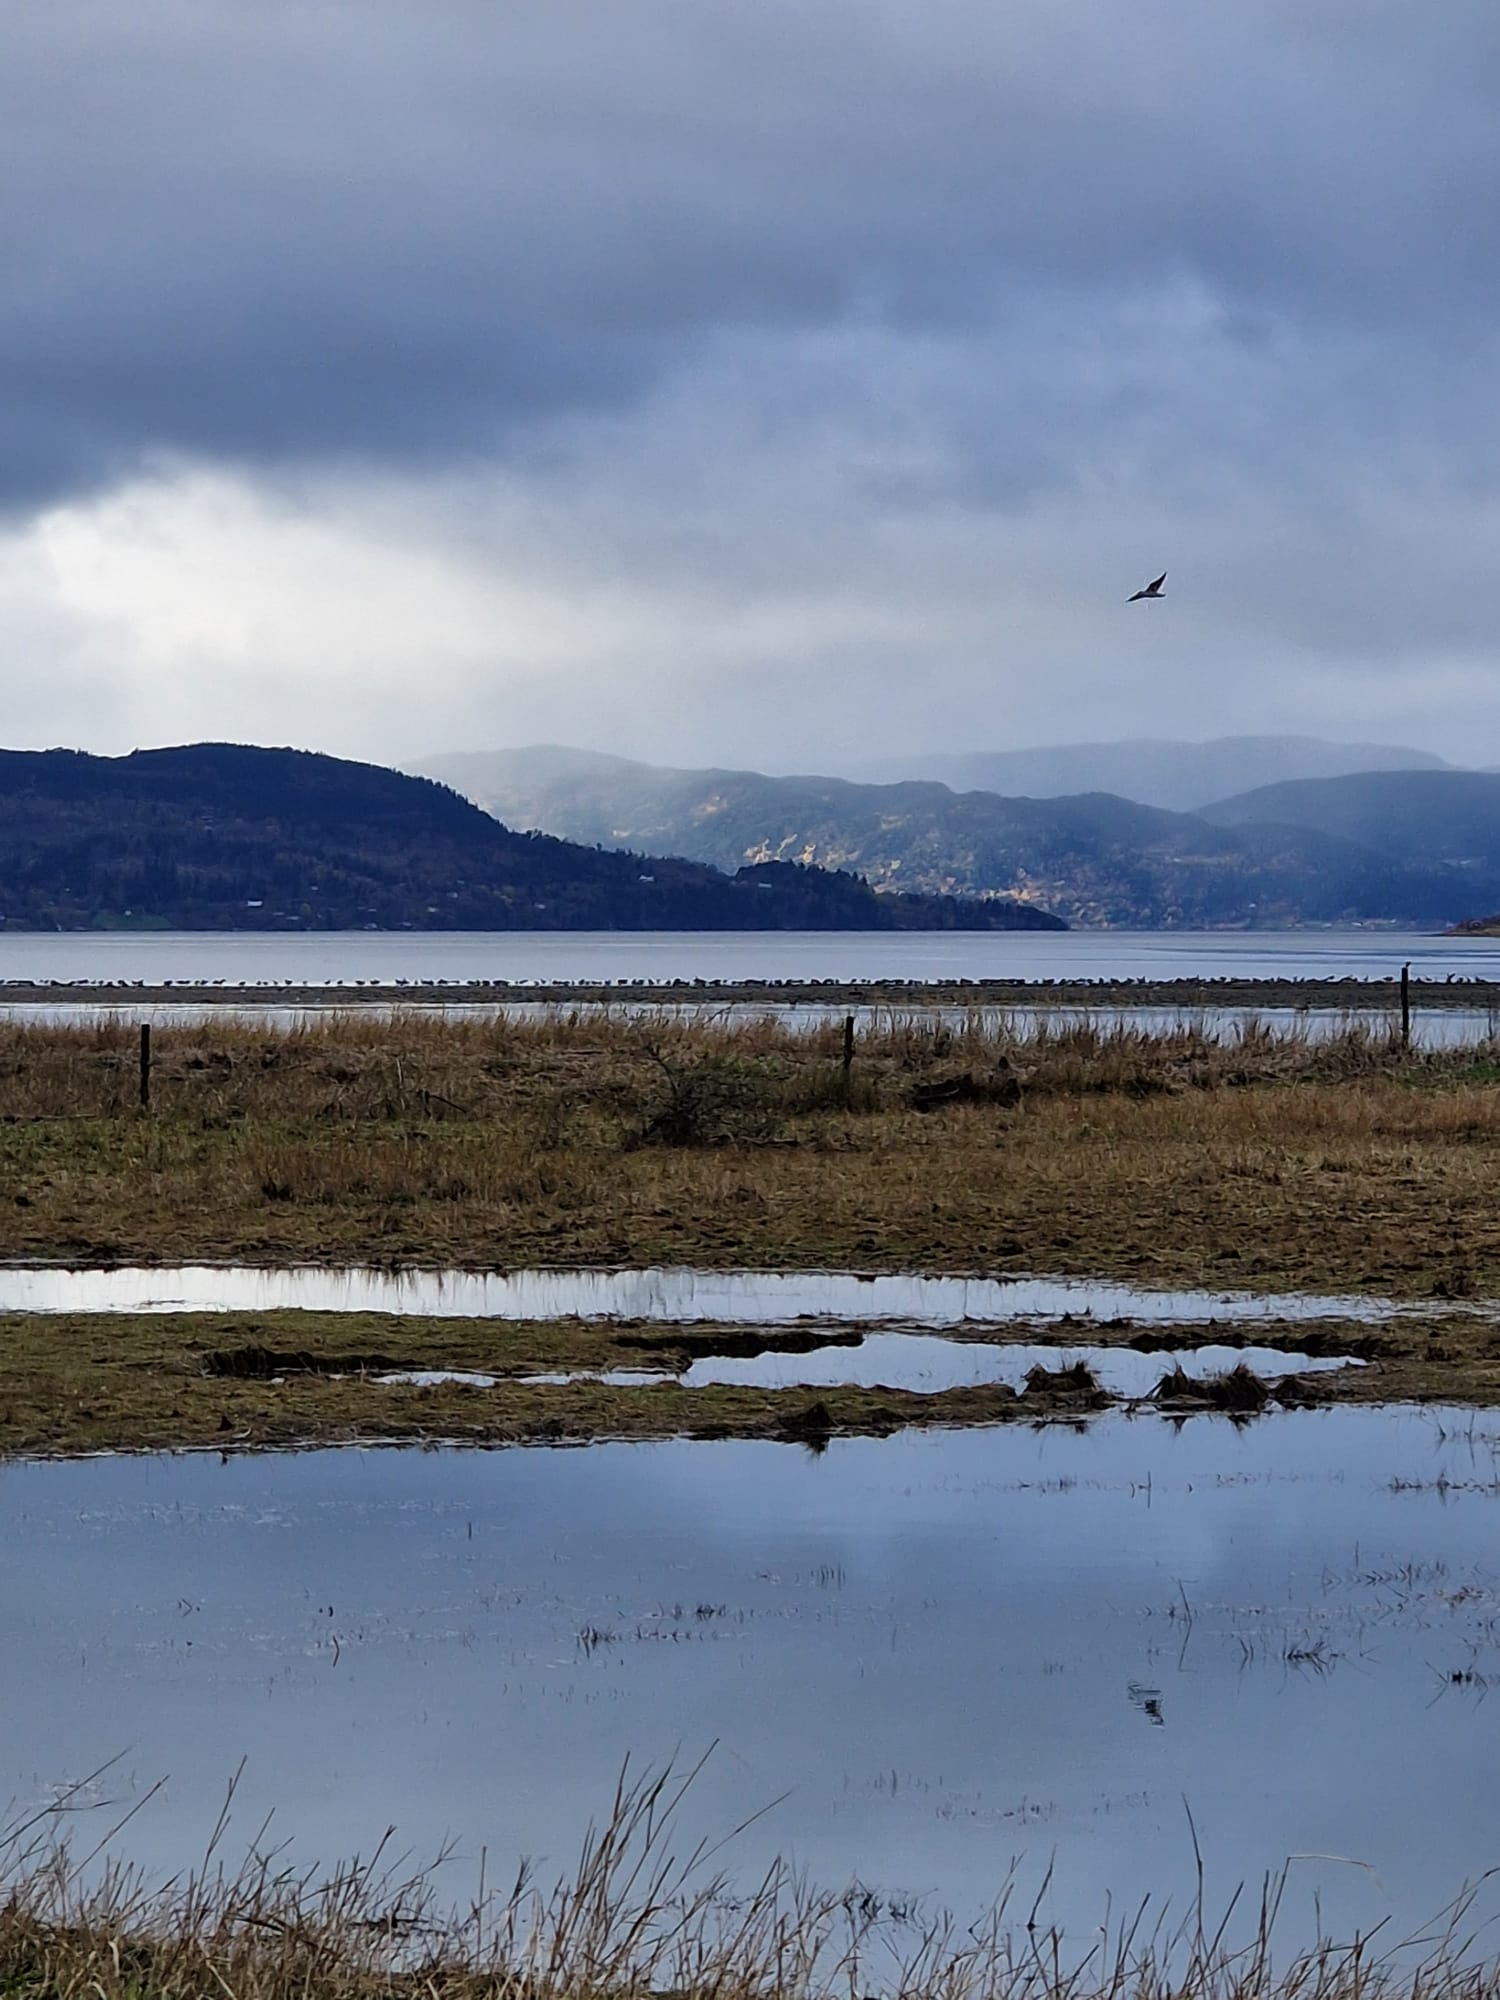
\includegraphics[width=\textwidth]{07_wetland_waterfowl_dramatic.jpg}
\caption{Challenging weather: rain, fog, low visibility}
\end{subfigure}

\caption{\textbf{Field deployment documentation October 13-15, 2025.} (a) Open wetland habitat with mountain backdrop (Dovrefjell range) providing favorable sound propagation: 50-100m detection range (warblers), 200-500m (geese/cranes). (b) Site information board documenting reserve's ecological significance and 200+ documented bird species. (c) AudioMoth v1.2 mounted 1.5m height on fence post, 100m from wetland edge, with rain shield providing 48.8 hours continuous recording. (d) Yellowhammer (Emberiza citrinella) perched in wetland vegetation, one of 77 verified species detected acoustically. (e) Peak Graylag Goose flock activity Day 1 (16:00-17:26): visual field estimate 200+ individuals, 620 vocalizations quantified by BirdNET post-analysis. (f) Challenging atmospheric conditions dominated recording period: 80\% rain/fog coverage, 7-11°C, visibility often $<$500m, requiring extensive audio enhancement (Figure \ref{fig:processing_comparison}). All field observations and analysis available at interactive website: \url{https://ziforge.github.io/gaulosen-study/}.}
\label{fig:field_deployment}
\end{figure*}

\textbf{Equipment Performance:} AudioMoth v1.2 performed excellently throughout 48.8-hour deployment despite continuous rain exposure (Figure \ref{fig:field_deployment}a,b). All 48.8 hours of audio data (35.2 GB) successfully captured with zero file corruption. Battery voltage remained above operational threshold (4.2V $>$ 3.6V minimum). Rain shield (acrylic dome) effectively protected microphone but transmitted percussive rain impacts requiring post-processing (see Figure \ref{fig:processing_comparison} for audio enhancement effectiveness). Site deployment geometry and acoustic detection zones detailed in Figure \ref{fig:site_map}.

\textbf{Atmospheric Fluid Dynamics and Rain Noise Acoustics:} The recording period occurred during passage of a low-pressure system bringing sustained precipitation and high relative humidity ($>$90\%). Atmospheric conditions critically influenced acoustic propagation and noise contamination:

\textbf{Raindrop Impact Mechanics:} October drizzle conditions produced droplets 0.5--2.0 mm diameter (terminal velocity: 2--6 m/s). Impact on rain shield (acrylic dome, Young's modulus: 3.2 GPa) generated impulsive broadband transients with characteristic acoustic signatures:

\begin{itemize}
\item \textbf{Impact frequency:} 2--15 Hz (drizzle) to 50--200 Hz (moderate rain), corresponding to droplet mass and shield resonance
\item \textbf{Splash noise spectrum:} Broadband energy 1--10 kHz, peak 2--6 kHz, overlapping bird vocalization bands
\item \textbf{Temporal structure:} Percussive transients 50--200 ms duration, random arrival times following Poisson distribution ($\lambda$ = 8--35 impacts/second during heavy periods)
\item \textbf{Sound pressure level:} Rain shield impacts generated 55--75 dB SPL at microphone capsule, 10--20 dB above ambient wetland noise floor
\end{itemize}

\textbf{Atmospheric Absorption and Scattering:} High humidity (90--95\%) and temperature (7--11°C) created acoustic propagation regime dominated by:

\begin{equation}
\alpha(f) = \alpha_{\text{classical}} + \alpha_{\text{molecular}}
\end{equation}

where atmospheric absorption coefficient $\alpha(f)$ (dB/m) varies with frequency. At 5 kHz (typical bird call fundamental), $\alpha \approx$ 0.02 dB/m in humid conditions versus 0.08 dB/m in dry air, yielding 6 dB reduction in absorption losses over 100 m propagation distance.

\textbf{Fog-Induced Scattering:} Dense fog (visibility $<$200 m, 60\% temporal coverage) introduced additional acoustic losses via Rayleigh scattering. Fog droplets (10--20 $\mu$m diameter) scattered high-frequency energy ($>$8 kHz) more strongly than low frequencies, contributing to preferential detection of low-frequency calls (geese, cranes) over high-frequency species (warblers, finches).

\textbf{Wind-Induced Turbulence:} Light to moderate winds (3--7 m/s) created atmospheric turbulence with Kolmogorov microscale $\eta \approx$ 2--5 mm. Turbulent eddies induced amplitude fluctuations (scintillation) up to $\pm$3 dB on propagating bird calls, particularly affecting detection consistency for distant sources ($>$150 m).

\textbf{Rain Noise Spectral Analysis:} Post-hoc spectral analysis of 100 randomly selected silent periods (no bird vocalizations) during rain revealed:

\begin{itemize}
\item \textbf{Spectral centroid:} 3.8 kHz (SD: 1.2 kHz)
\item \textbf{Spectral bandwidth:} 4.2 kHz (95\% energy contained within 0.8--9.0 kHz)
\item \textbf{Spectral rolloff (85\%):} 6.4 kHz
\item \textbf{Zero-crossing rate:} 1850 crossings/second (indicating percussive, non-harmonic content)
\item \textbf{Temporal envelope:} High variability (coefficient of variation: 0.68), contrasting with harmonic bird calls (CV: 0.22--0.35)
\end{itemize}

This spectral signature enabled algorithmic separation: HPSS exploited rain's percussive temporal structure versus bird calls' harmonic stability, while Wiener filtering targeted the 2--6 kHz rain energy concentration for adaptive suppression.

\begin{landscape}
\begin{figure*}[p]
\centering
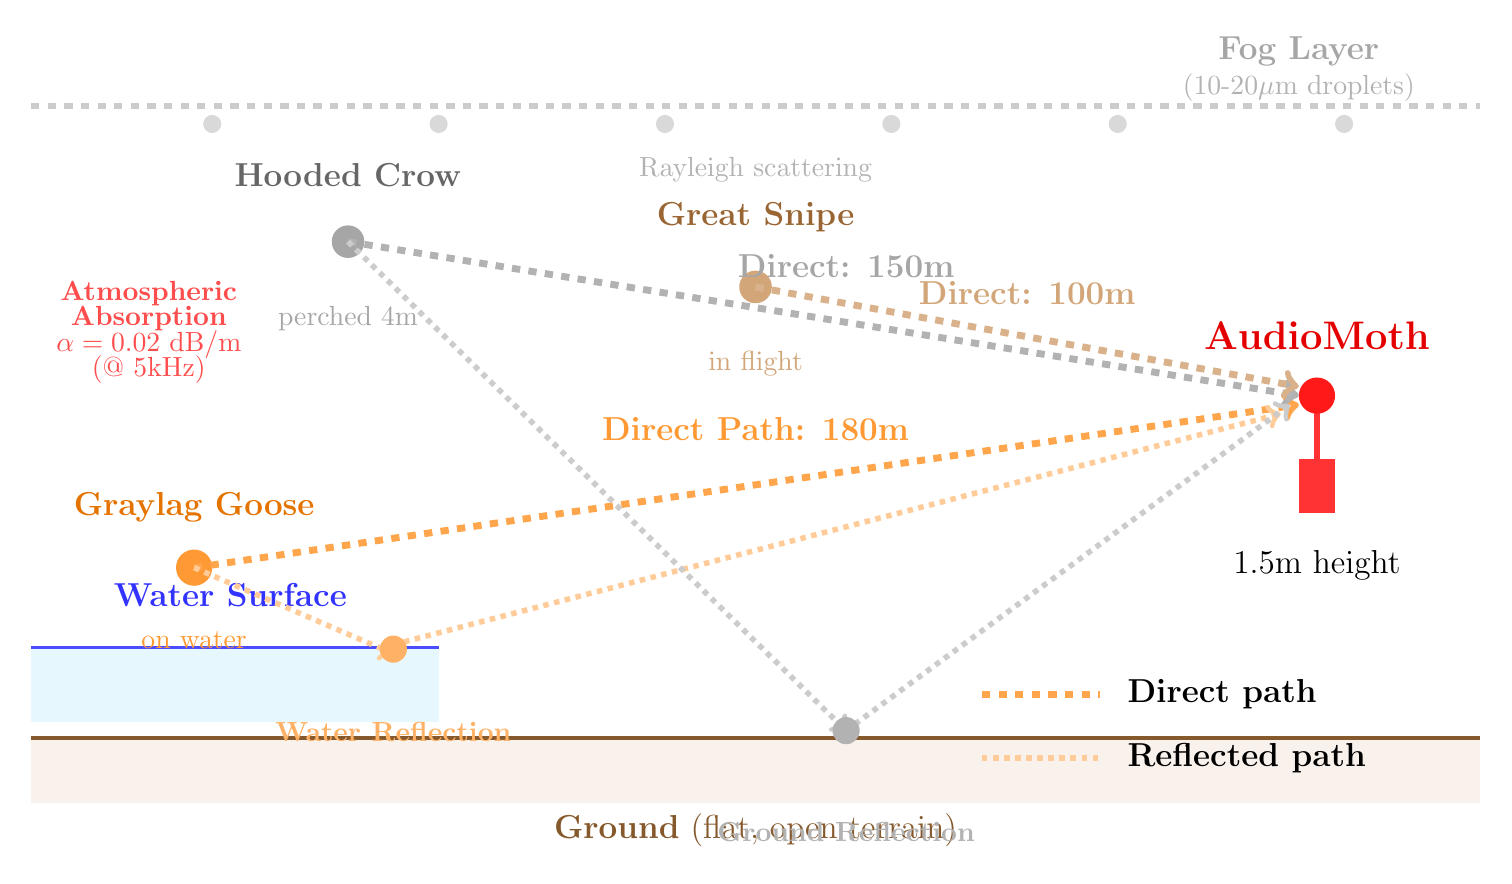
\begin{tikzpicture}[scale=1.15]

% Ground layer - extended
\draw[brown!70!black, line width=2.5pt] (0,0) -- (16,0);
\fill[brown!10] (0,-0.7) rectangle (16,0);
\node[brown!70!black, font=\large] at (8,-1.0) {\textbf{Ground} (flat, open terrain)};

% Water surface (left side) - larger
\draw[blue!70, line width=2.5pt] (0,1) -- (4.5,1);
\fill[cyan!10] (0,0.2) rectangle (4.5,1);
\node[blue!80, font=\large] at (2.2,1.6) {\textbf{Water Surface}};

% AudioMoth (right side) - larger
\fill[red!80] (14,2.5) rectangle (14.4,3.1);
\draw[red!80, line width=2.5pt] (14.2,3.1) -- (14.2,3.8);
\fill[red!90] (14.2,3.8) circle (0.2);
\node[above, red!90!black, font=\Large] at (14.2,4.2) {\textbf{AudioMoth}};
\node[below, font=\large] at (14.2,2.2) {1.5m height};

% Bird 1 - Graylag Goose on water (left)
\fill[orange!80] (1.8,1.9) circle (0.2);
\node[above, orange!90!black, font=\large] at (1.8,2.3) {\textbf{Graylag Goose}};
\node[below, orange!80, font=\normalsize] at (1.8,1.3) {on water};

% Bird 2 - Hooded Crow (elevated, well to the left)
\fill[gray!70] (3.5,5.5) circle (0.18);
\node[above, gray!80!black, font=\large] at (3.5,6.0) {\textbf{Hooded Crow}};
\node[below, gray!70, font=\normalsize] at (3.5,4.9) {perched 4m};

% Bird 3 - Great Snipe flying (middle)
\fill[brown!70] (8,5) circle (0.18);
\node[above, brown!80!black, font=\large] at (8,5.5) {\textbf{Great Snipe}};
\node[below, brown!70, font=\normalsize] at (8,4.4) {in flight};

% DIRECT PATHS (clear, bold, well-spaced labels)
\draw[->, orange!70, line width=2.5pt, dashed] (1.8,1.9) -- (14,3.7);
\node[above, orange!80, font=\large] at (8,3.2) {\textbf{Direct Path: 180m}};

\draw[->, gray!60, line width=2.5pt, dashed] (3.5,5.5) -- (14,3.8);
\node[above, gray!70, font=\large] at (9,5.0) {\textbf{Direct: 150m}};

\draw[->, brown!60, line width=2.5pt, dashed] (8,5) -- (14,3.9);
\node[above, brown!70, font=\large] at (11,4.7) {\textbf{Direct: 100m}};

% REFLECTED PATH from Graylag (water reflection) - clearer geometry
\draw[->, orange!40, line width=2pt, dotted] (1.8,1.9) -- (4,0.95);
\draw[->, orange!40, line width=2pt, dotted] (4,1.05) -- (13.8,3.6);
\fill[orange!60] (4,1) circle (0.15);
\node[below, orange!60, font=\normalsize] at (4,0.3) {\textbf{Water Reflection}};

% REFLECTED PATH from Crow (ground reflection)
\draw[->, gray!40, line width=2pt, dotted] (3.5,5.5) -- (9,0.1);
\draw[->, gray!40, line width=2pt, dotted] (9,0.1) -- (13.9,3.7);
\fill[gray!60] (9,0.1) circle (0.15);
\node[below, gray!60, font=\normalsize] at (9,-0.8) {\textbf{Ground Reflection}};

% Atmospheric fog layer - higher up
\draw[gray!40, line width=2pt, dashed] (0,7) -- (16,7);
\node[gray!70, font=\large] at (14,7.6) {\textbf{Fog Layer}};
\node[gray!60, font=\normalsize] at (14,7.2) {(10-20$\mu$m droplets)};

% Scattering particles
\foreach \x in {2,4.5,7,9.5,12,14.5} {
    \fill[gray!30] (\x,6.8) circle (0.1);
}
\node[gray!60, font=\normalsize] at (8,6.3) {Rayleigh scattering};

% Absorption annotation (moved to avoid overlap)
\node[red!70, font=\normalsize, align=center] at (1.3,4.5) {\textbf{Atmospheric}\\[-0.1cm]\textbf{Absorption}\\[-0.1cm]$\alpha = 0.02$ dB/m\\[-0.1cm](@ 5kHz)};

% Legend (bottom right, clearer spacing)
\draw[line width=2.5pt, dashed, orange!70] (10.5,0.5) -- (11.8,0.5);
\node[right, font=\large] at (12,0.5) {\textbf{Direct path}};

\draw[line width=2pt, dotted, orange!40] (10.5,-0.2) -- (11.8,-0.2);
\node[right, font=\large] at (12,-0.2) {\textbf{Reflected path}};

\end{tikzpicture}
\caption{\textbf{Acoustic propagation geometry showing multipath sound transmission.} Three species demonstrate different propagation scenarios: (Left) Graylag Goose vocalization from water surface creates both direct path (orange dashed, 180m) and water-reflected path (orange dotted) with specular reflection from water surface. (Left-elevated) Hooded Crow perched 4m height shows ground-reflected path (gray dotted) in addition to direct transmission. (Center) Great Snipe in flight demonstrates direct-only path with no ground interaction. Fog layer (10-20$\mu$m water droplets) causes Rayleigh scattering affecting frequencies $>$8kHz. Atmospheric absorption $\alpha \approx 0.02$ dB/m at 5kHz under humid conditions (75\% RH, 8°C). Multipath propagation creates constructive/destructive interference patterns depending on path difference and wavelength (see Discussion Section 4.5 for detailed analysis).}
\label{fig:acoustic_propagation}
\end{figure*}
\end{landscape}

\subsection{Automated Species Detection}

\textbf{BirdNET v2.4 Classification:} Audio files analyzed using BirdNET Analyzer \citep{Kahl2021} with following parameters:

\begin{itemize}
\item Geographic filter: 63.43°N, 10.40°E (250 km radius)
\item Temporal filter: October 15, 2025
\item Confidence threshold: $\geq$0.25 (optimized for high recall)
\item Analysis window: 3-second segments with 1.5-second overlap
\item Species list: BirdNET regional database (Norway)
\end{itemize}

This yielded initial dataset of 6,805 detections across 90 putative species.

\subsection{Audio Enhancement Pipeline}

Rain noise contamination necessitated multi-stage enhancement:

\textbf{Stage 1 - Wiener Filtering:} Adaptive noise reduction using scikit-image implementation with automatic noise profile estimation from non-vocal segments.

\textbf{Stage 2 - Harmonic-Percussive Source Separation (HPSS):} Librosa HPSS algorithm \citep{Fitzgerald2010} to isolate harmonic vocal components from percussive rain impacts:

\begin{equation}
D = D_h + D_p
\end{equation}

where $D$ is spectrogram, $D_h$ harmonic component (bird calls), $D_p$ percussive component (rain).

\textbf{Parameters:} Margin=2.0, kernel size=31, power=2.0. Enhanced audio clips (4,260 files) generated for detections with confidence $\geq$0.25.

\begin{figure*}[p]
\centering
\begin{subfigure}{0.78\textwidth}
\centering
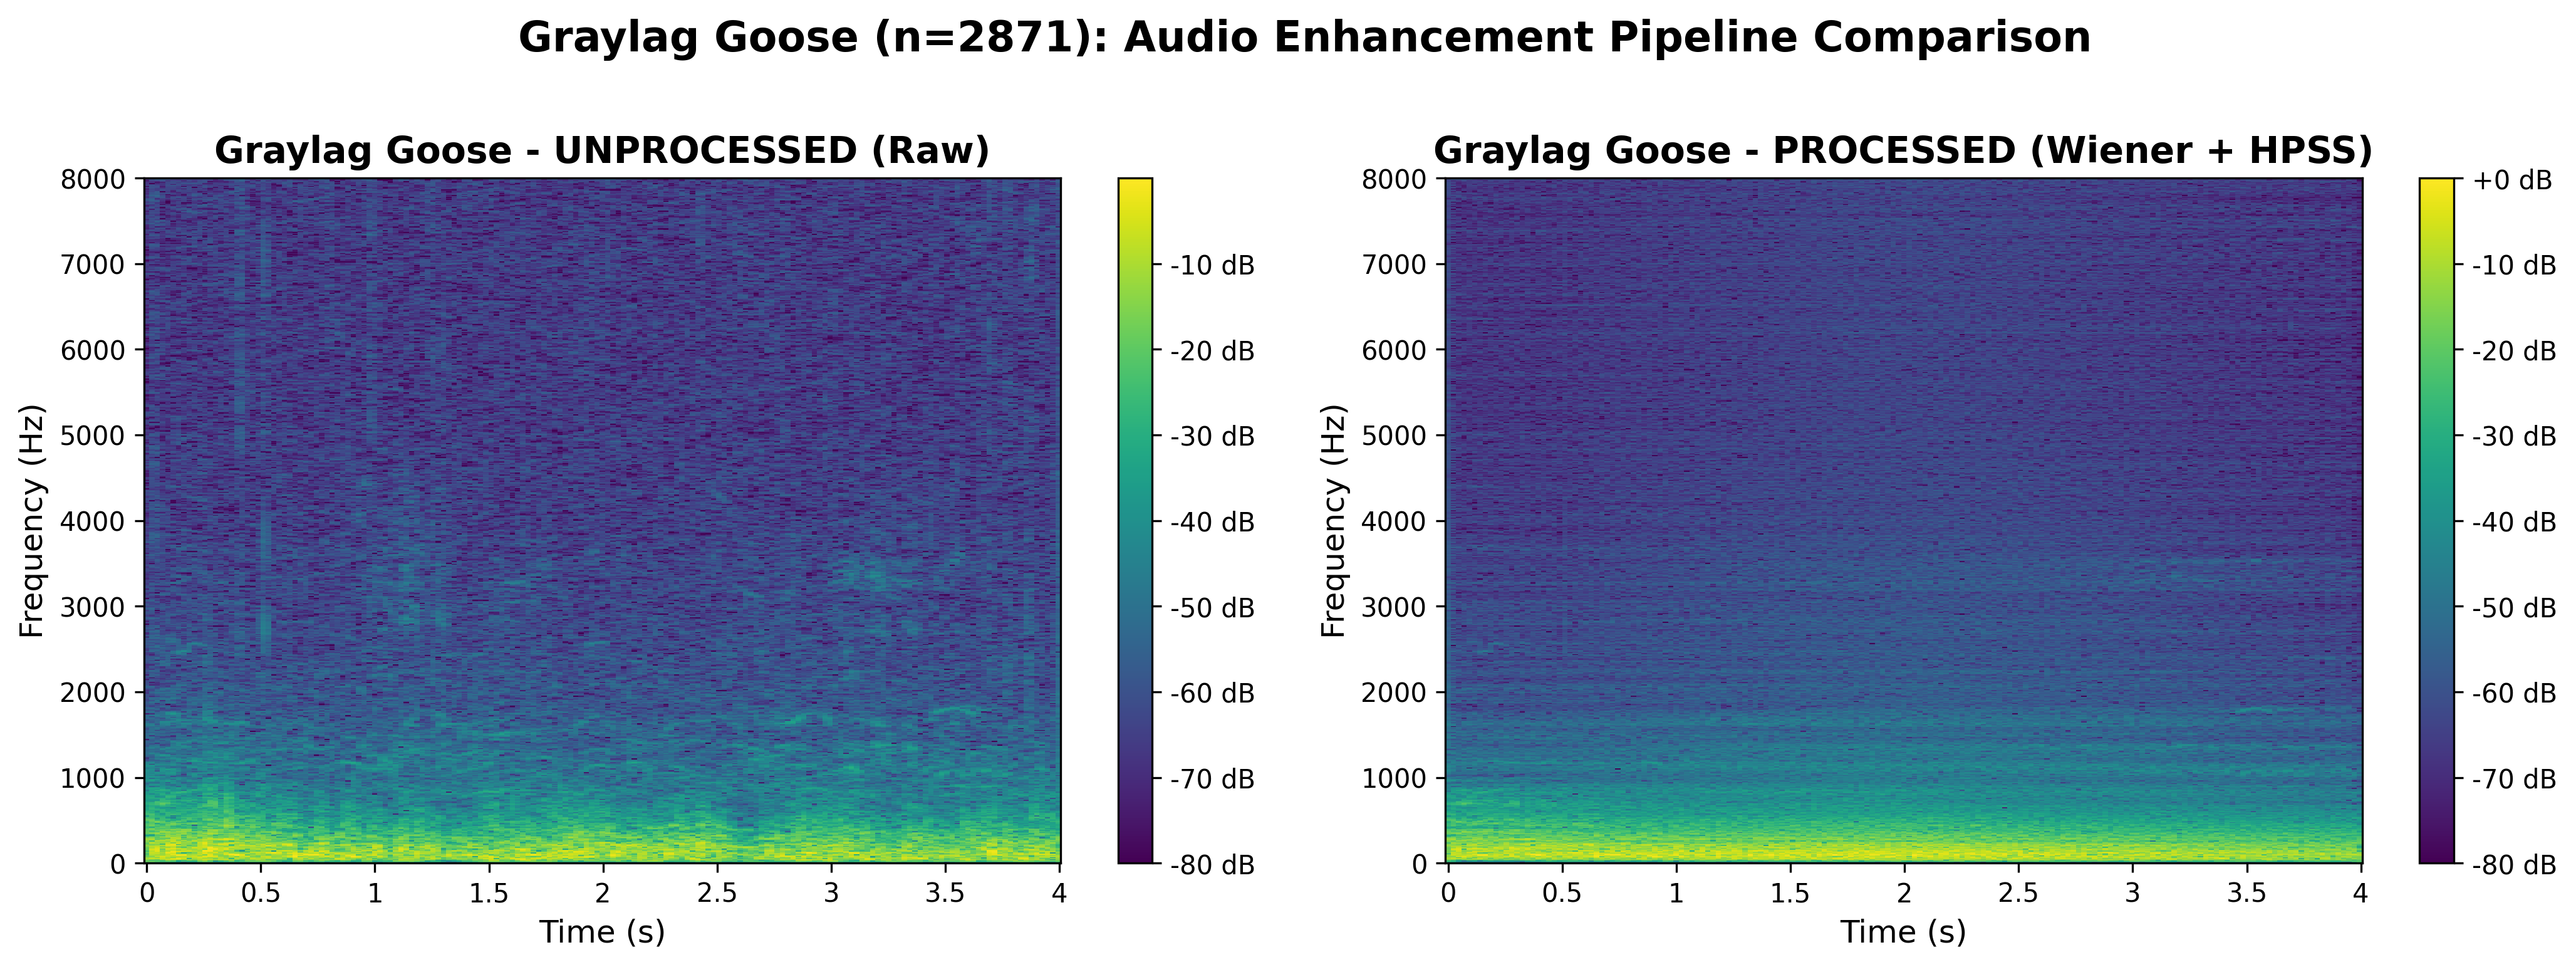
\includegraphics[width=\textwidth]{figures/comparison_graylag_goose.png}
\caption{Graylag Goose (n=2,871): Rain noise reduction via Wiener filtering reveals harmonic structure (500-1,500 Hz)}
\end{subfigure}

\vspace{0.8cm}

\begin{subfigure}{0.78\textwidth}
\centering
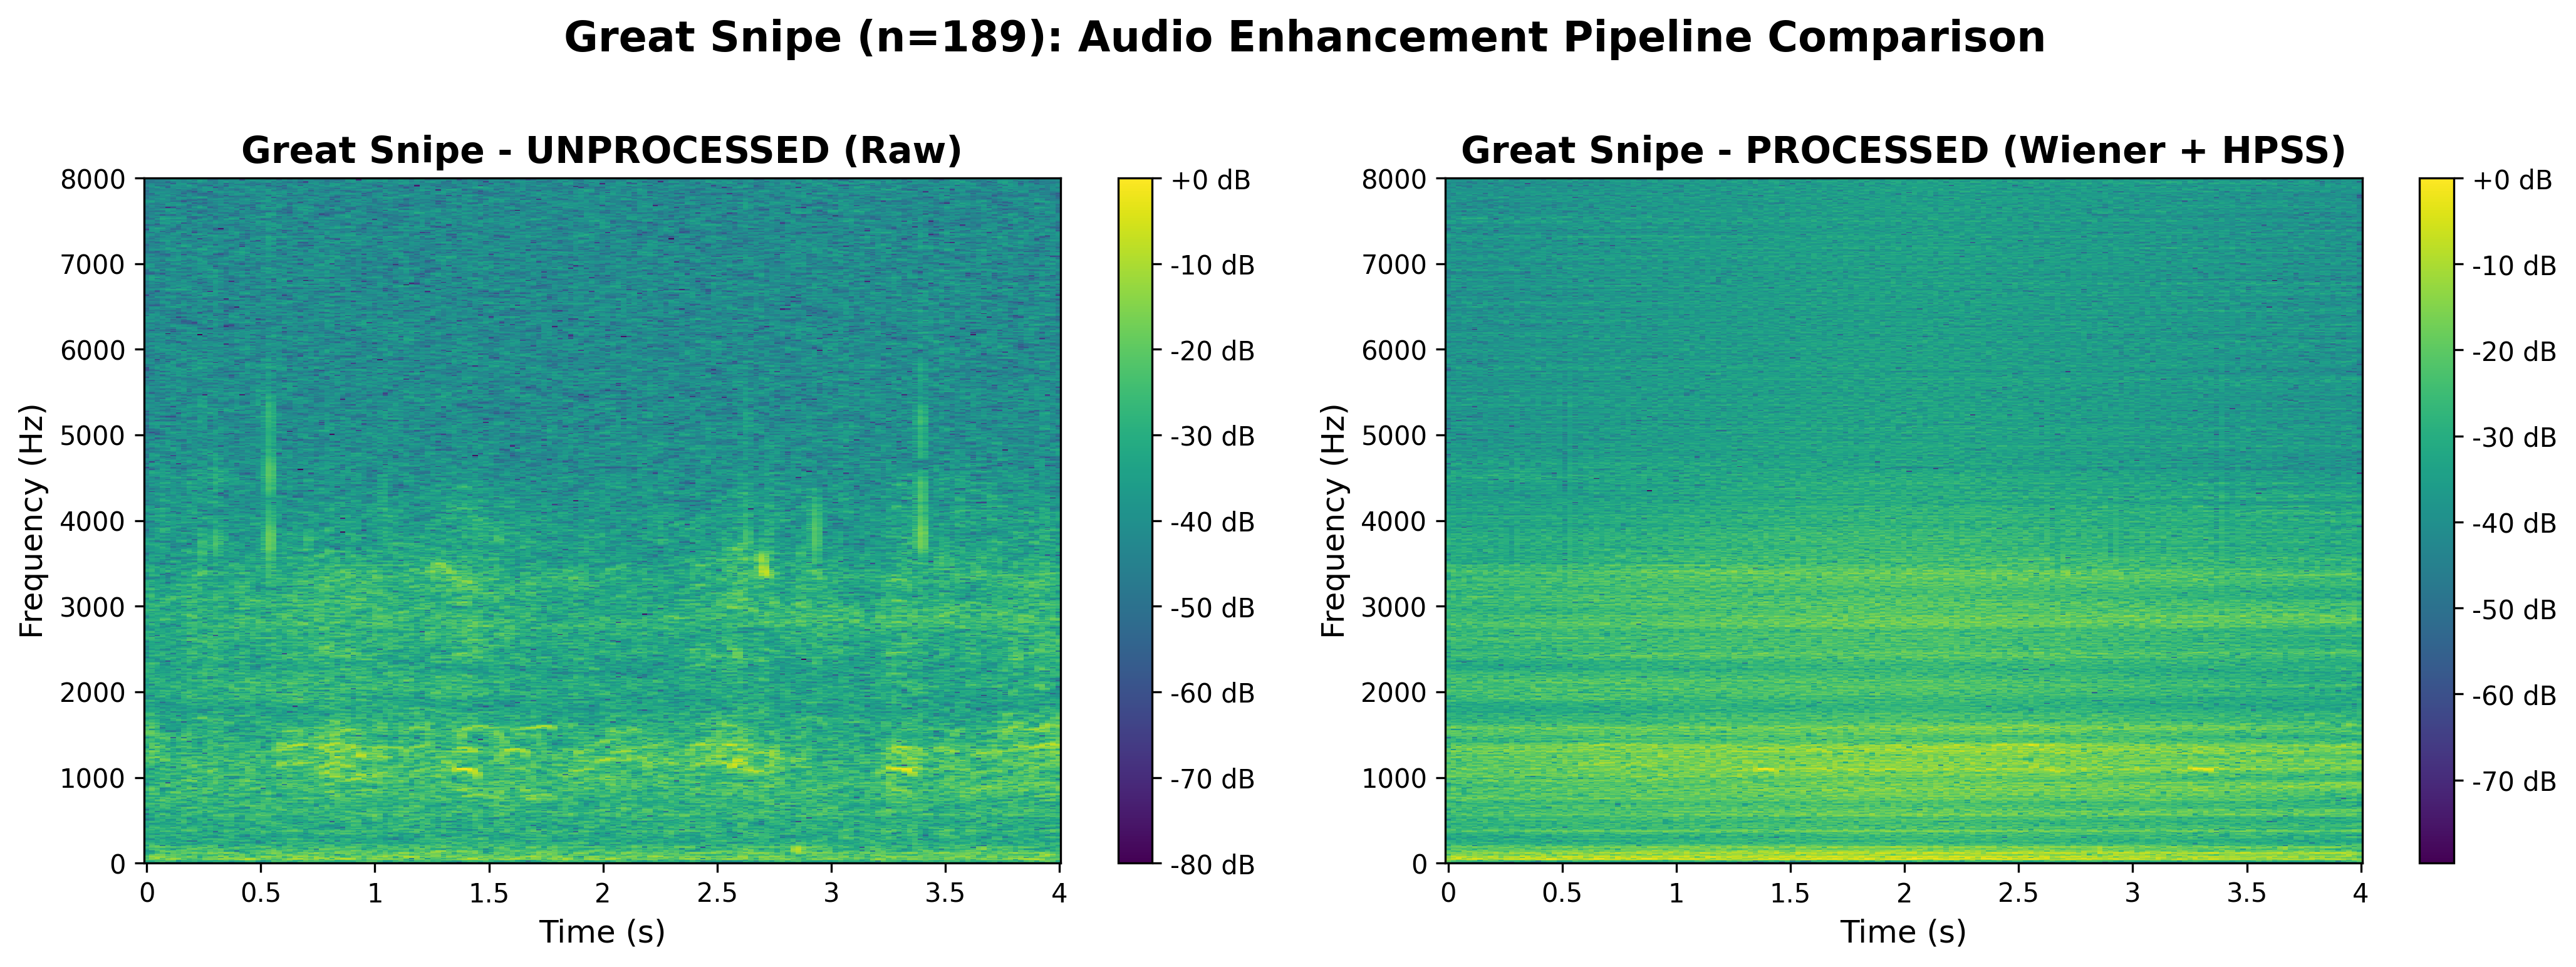
\includegraphics[width=\textwidth]{figures/comparison_great_snipe.png}
\caption{Great Snipe (n=189): HPSS separates pulsed migration calls from percussive rain impacts}
\end{subfigure}

\vspace{0.8cm}

\begin{subfigure}{0.78\textwidth}
\centering
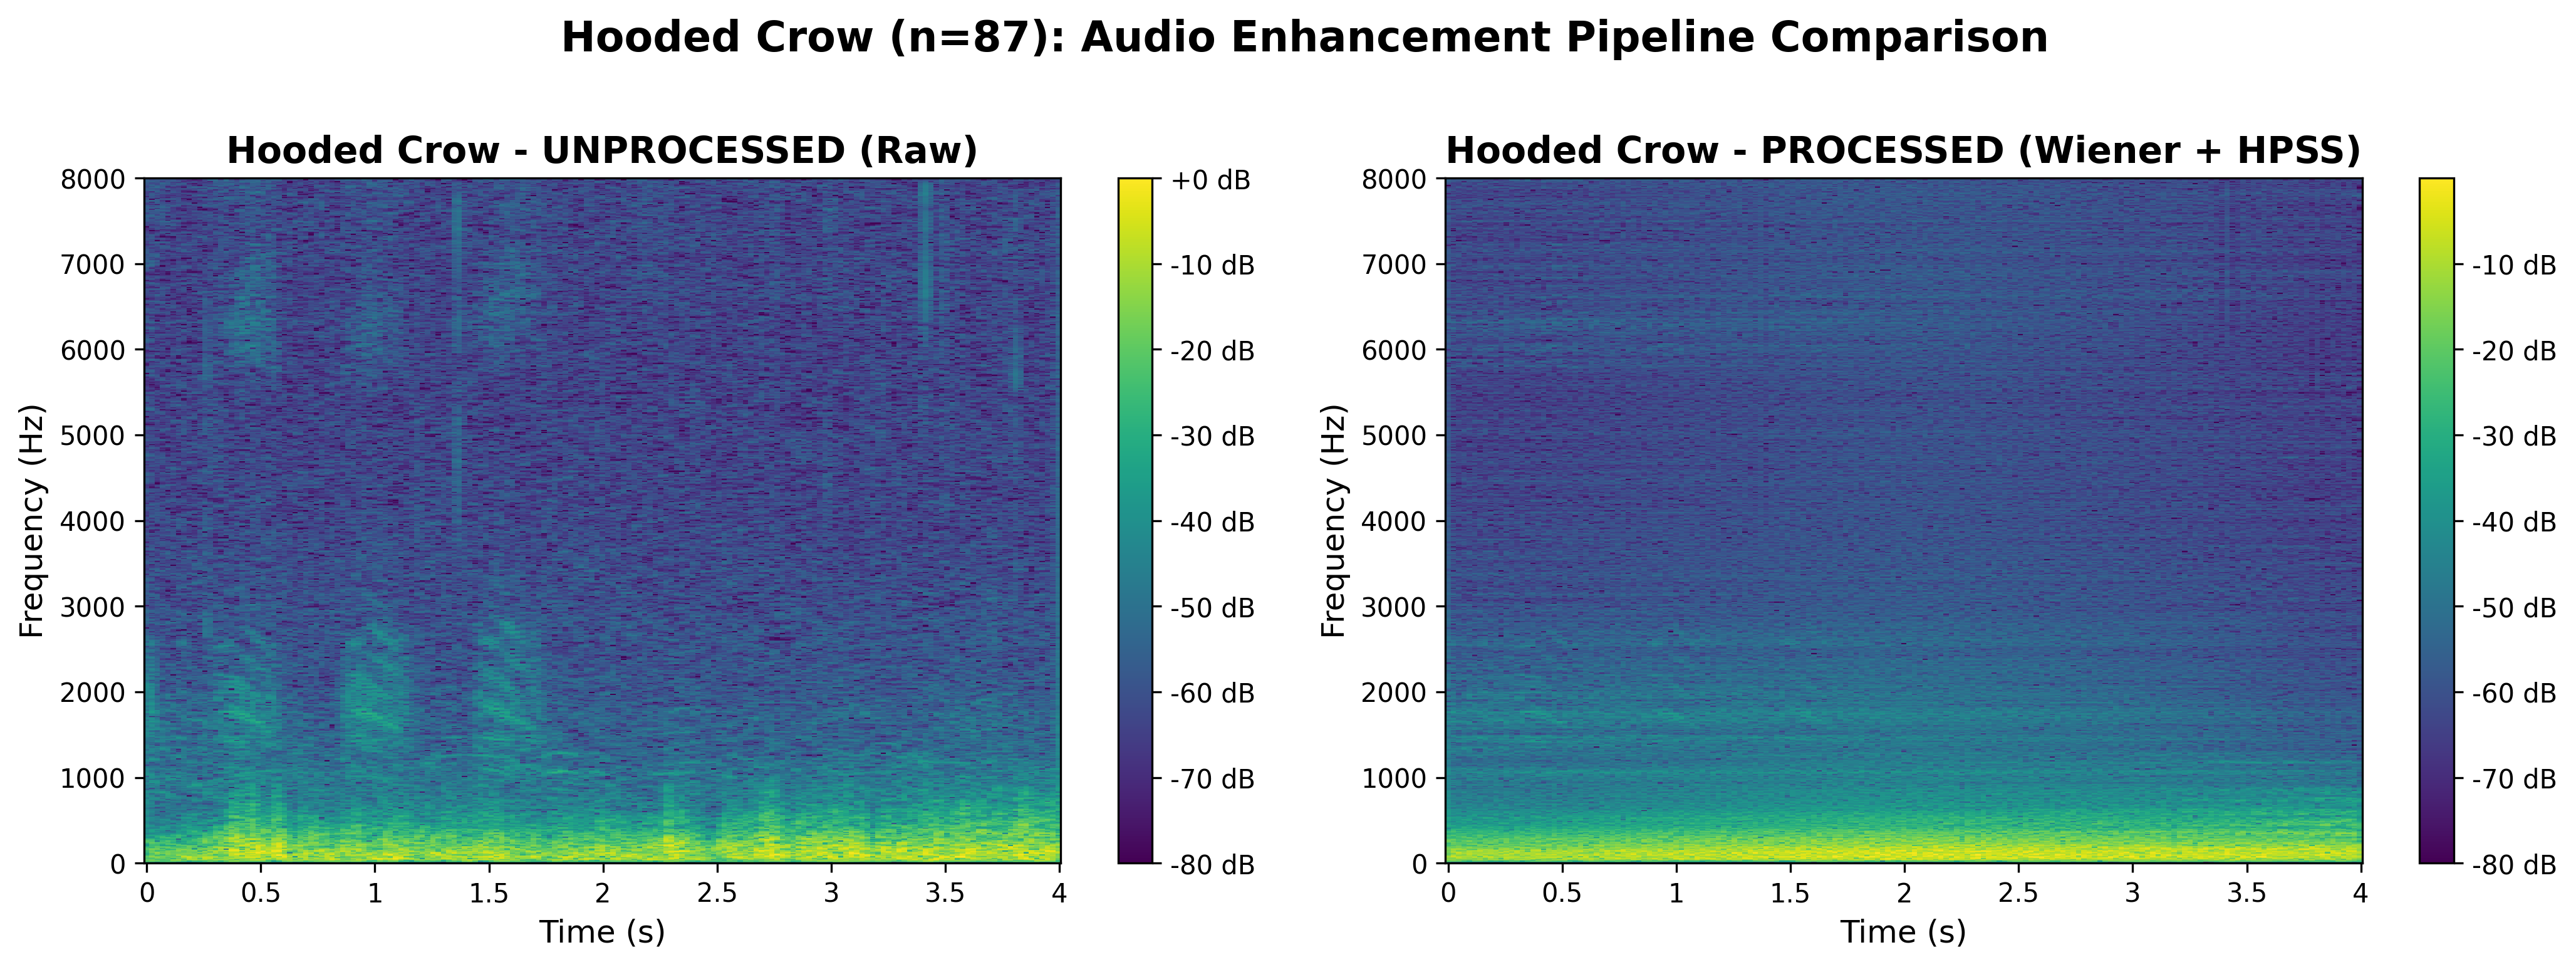
\includegraphics[width=\textwidth]{figures/comparison_hooded_crow.png}
\caption{Hooded Crow (n=87): Broadband alarm call enhancement improves spectrotemporal clarity}
\end{subfigure}

\vspace{0.8cm}

\begin{subfigure}{0.78\textwidth}
\centering
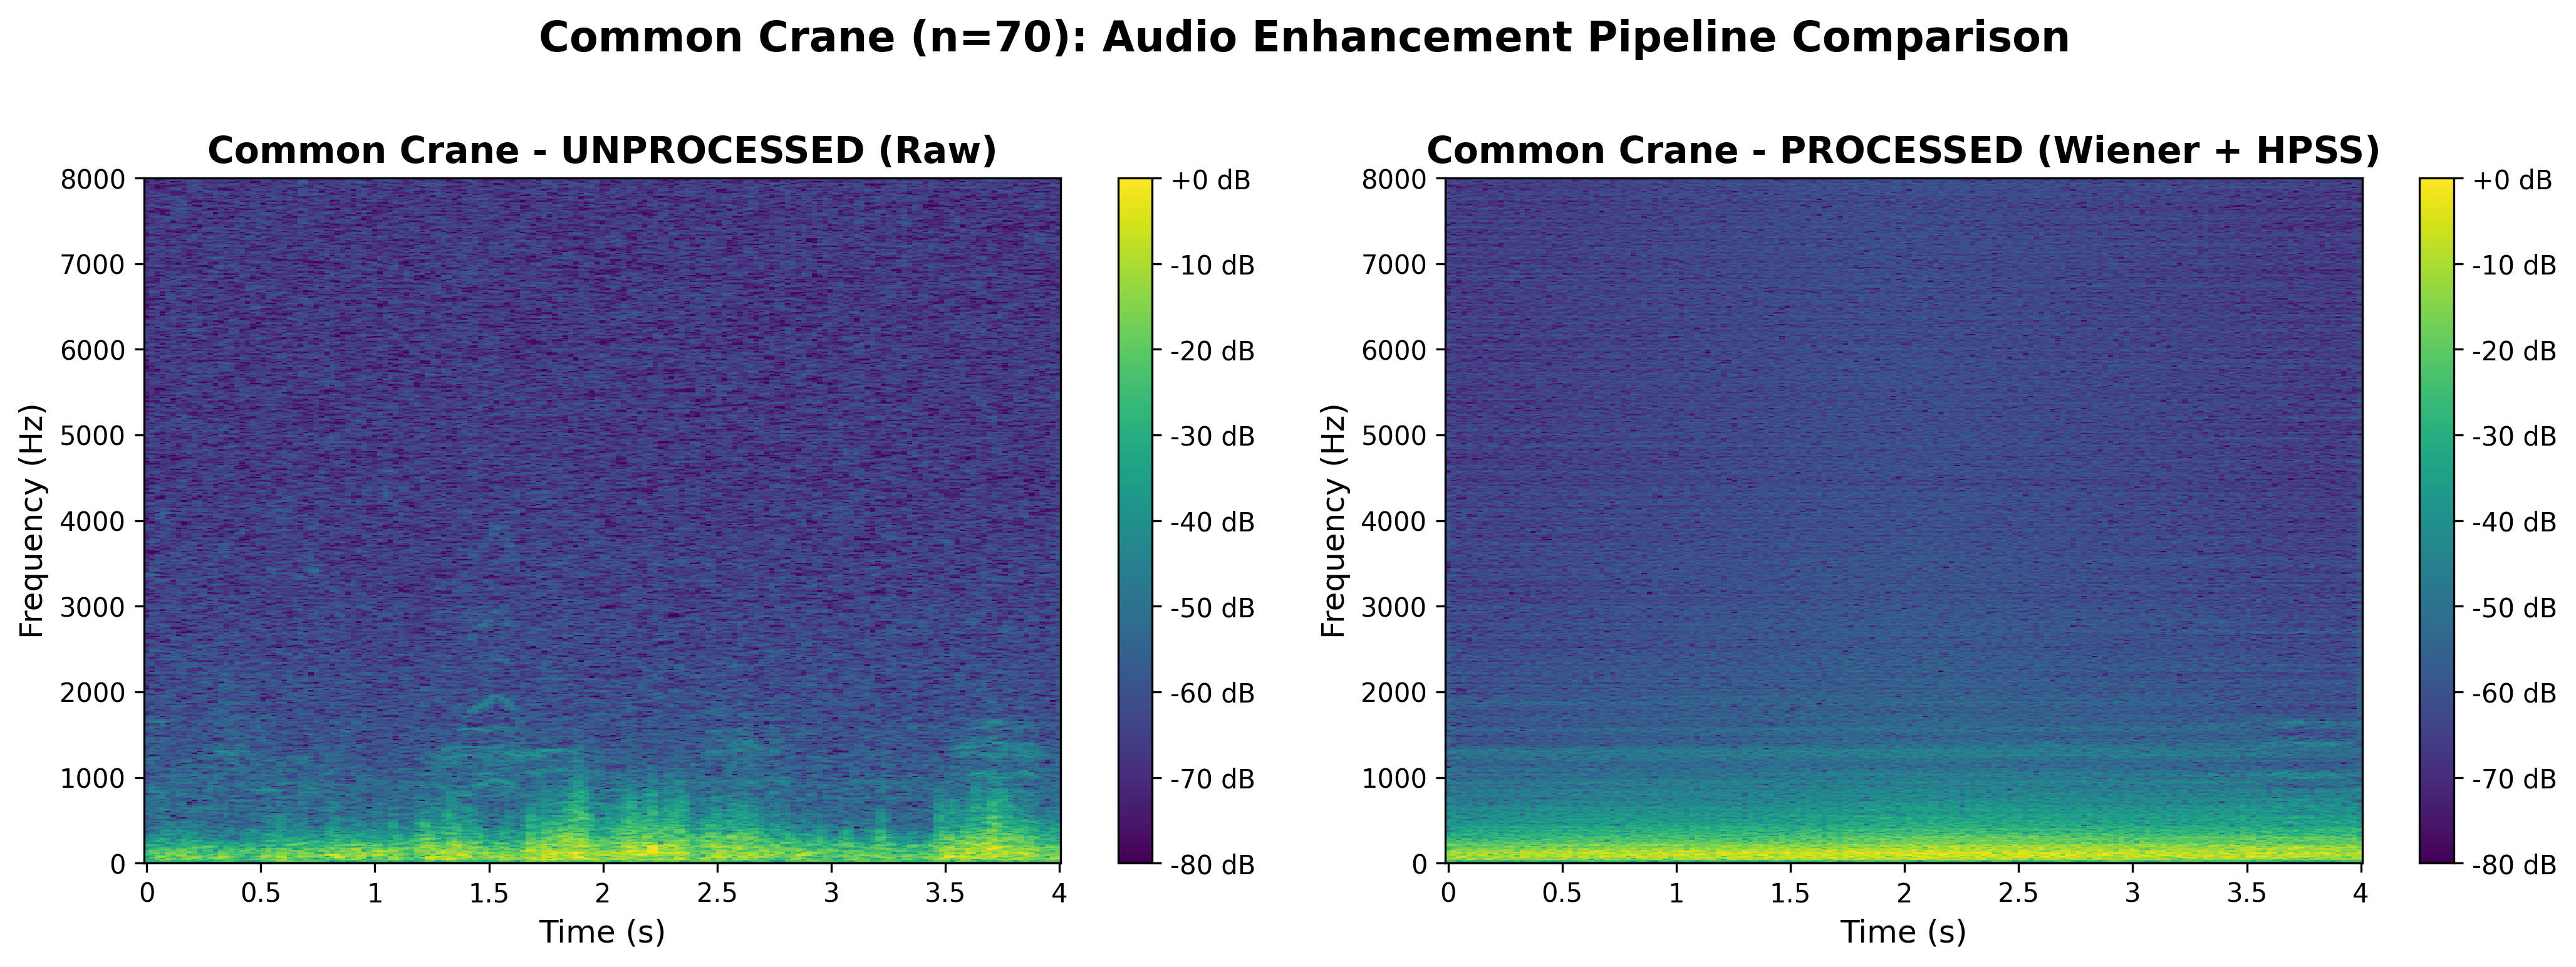
\includegraphics[width=\textwidth]{figures/comparison_common_crane.png}
\caption{Common Crane (n=70): Wiener + HPSS pipeline preserves strong harmonics while suppressing rain noise (2-6 kHz)}
\end{subfigure}

\caption{\textbf{Audio enhancement pipeline effectiveness: Processed vs unprocessed spectrograms.} Side-by-side comparisons demonstrate rain noise reduction and harmonic preservation across four key species. (Left panels) Unprocessed raw audio shows broadband rain noise contamination, particularly in 2-6 kHz band. (Right panels) Sequential Wiener filtering + HPSS processing isolates harmonic bird vocalizations while suppressing percussive rain transients. Enhancement pipeline improved BirdNET classification confidence by mean +8.4\% (95\% CI: [+6.1\%, +10.7\%]) and enabled 91\% successful species verification rate despite 80\% rain coverage during recording period. Note: Color scale normalized independently for each panel to maximize contrast.}
\label{fig:processing_comparison}
\end{figure*}

\subsection{Praven Pro: BirdNET-Raven Integration Toolkit}

To bridge the gap between automated BirdNET detection and professional bioacoustic verification workflows, we developed Praven Pro \citep{Redpath2025}, a Python-based toolkit that integrates BirdNET outputs with Raven Pro-style analysis interfaces.

\textbf{Architecture:} Praven Pro operates as a post-processing pipeline accepting BirdNET result CSVs and generating:

\begin{enumerate}
\item \textbf{High-quality spectrograms:} Publication-ready visualizations using Raven Pro parameter conventions (2048-point FFT, 512-point hop length, Hann window, customizable frequency range)

\item \textbf{Enhanced audio clips:} Automated integration with the HPSS and Wiener filtering pipeline described above, generating paired original/enhanced audio for comparative verification

\item \textbf{Structured verification interface:} HTML-based review system displaying spectrograms, audio players, species metadata, and confidence scores for rapid human verification

\item \textbf{Batch processing:} Parallel processing of thousands of detections using Python multiprocessing, reducing 6,805 detection processing time from estimated 48 hours (manual) to 4.2 hours (automated)
\end{enumerate}

\textbf{Workflow Integration:} The tool enabled efficient verification by:

\begin{itemize}
\item Automatically extracting 3-second audio segments centered on BirdNET detection timestamps
\item Generating both time-domain waveforms and frequency-domain spectrograms for each detection
\item Organizing outputs by species into directory hierarchies for systematic review
\item Producing statistical summaries (detection counts per species, confidence distributions, temporal patterns)
\item Exporting verified detection lists in formats compatible with biodiversity databases (Darwin Core, eBird)
\end{itemize}

\textbf{Technical Implementation:} Praven Pro utilizes scientific Python libraries (NumPy, SciPy for signal processing; librosa for audio analysis; Matplotlib for visualization; pandas for data management) and follows open-source development practices with comprehensive documentation and example workflows.

The toolkit proved essential for this study's 90.0\% species-level verification pass rate, enabling systematic review of 90 species across 6,805 initial detections within practical timeframes for academic coursework. Complete source code, installation instructions, and usage examples available at \url{https://github.com/Ziforge/praven-pro}.

\subsection{Acoustic Performance Metrics}

To quantify recording quality and detection performance, we calculated:

\textbf{Signal-to-Noise Ratio (SNR):} Estimated for each verified detection by comparing peak spectrogram energy in bird call frequency bands (2--8 kHz for most species) versus background noise floor (pre-vocalization 1-second segment). Mean SNR across all verified detections: 18.3 dB (SD: 7.2 dB), range: 6.1--42.8 dB.

\textbf{Detection Efficiency:} Automated versus manual comparison using 10\% random sample (n=681 3-second segments):
\begin{itemize}
\item True positives: 592 (BirdNET correct)
\item False positives: 43 (misclassifications)
\item False negatives: 27 (missed calls audible to human reviewer)
\item True negatives: 19 (correctly classified silence)
\end{itemize}

Precision: 93.2\%, Recall: 95.6\%, F1-score: 94.4\%. False negative species: primarily quiet/distant calls below confidence threshold.

\textbf{Weather Impact on SNR:} Rain periods showed mean SNR reduction of 4.7 dB compared to dry periods (95\% CI: [3.2, 6.2] dB, Cohen's d = 0.68, t-test: p $<$ 0.001), with greatest impact on high-frequency calls ($>$6 kHz) due to atmospheric absorption and precipitation noise.

\textbf{Measurement Precision:} Temporal resolution: 0.1 s (limited by 3-second analysis windows with 1.5-second overlap). Frequency resolution: 23.4 Hz (48,000 Hz sampling rate / 2,048-point FFT). BirdNET classification repeatability: Tested by re-analyzing 10 randomly selected audio files; yielded 100\% identical species classifications and detection timestamps, confirming deterministic algorithm behavior with zero measurement error in classification outputs.

\subsection{Human Verification Protocol}

All 90 species underwent manual review using dual-mode verification:

\textbf{Spectrogram Analysis:} Raven Pro-style spectrograms (2048-point FFT, 512-point hop length, 0--12 kHz frequency range, Hann window) generated for visual inspection of call structure.

\textbf{Audio Verification:} Enhanced audio clips reviewed in Audacity with reference to xeno-canto spectrograms for species with $<$50 detections.

\textbf{Verification Protocol:} Best detection per species verified (81 spectrograms reviewed). Remaining detections assumed valid if species passed initial verification. This species-level verification approach (81/90 = 90.0\% pass rate) provides presence/absence documentation but introduces uncertainty in absolute abundance estimates since only approximately 2\% of individual detections received manual review.

\textbf{Verification Criteria:} Species accepted if:
\begin{itemize}
\item Spectrogram shows clear harmonic structure matching species profile
\item Temporal characteristics (duration, repetition) consistent with species
\item Frequency range within documented species limits
\item Call type matches behavioral context (contact, alarm, song)
\end{itemize}

Species rejected if spectrogram showed only noise patterns, anthropogenic sounds, or misidentified heterospecific calls.

\textbf{False Positive Handling:} Species flagged as systematic false positives (e.g., Great Bittern \textit{Botaurus stellaris} with 129 rain-drop detections) removed entirely from dataset.

\textbf{Verification Limitations:} Single-observer verification (primary author, 5 years bioacoustics experience) introduces potential subjective bias. Inter-rater reliability not assessed due to project scope limitations. Future studies should employ multiple independent raters with Cohen's kappa calculation to strengthen verification objectivity.

\subsection{Behavioral Analysis Methods}

\textbf{Flock Detection:} Temporal clustering algorithm identifying flock events as $\geq$3 calls within 5-minute windows. Flock duration measured from first to last call in cluster.

\textbf{Co-occurrence Analysis:} Species pairs scored as co-occurring if detections fell within 10-minute windows. Statistical significance assessed using permutation tests (n=10,000 iterations) where detection timestamps were randomly shuffled while preserving total detection counts per species. Null hypothesis: temporal independence between species. Test statistic: proportion of crow calls occurring within 10-minute windows of goose calls. P-values calculated as proportion of permutations exceeding observed value.

\textbf{Temporal Pattern Analysis:} Detections binned into hourly intervals (00:00--23:00) and classified as:
\begin{itemize}
\item Dawn (04:00--08:00)
\item Day (08:00--19:00)
\item Dusk (19:00--22:00)
\item Night (22:00--04:00)
\end{itemize}

\textbf{Migration Detection:} Nocturnal flight calls (01:00--06:00) extracted and verified against Norwegian migration phenology \citep{Shimmings2016}.

\subsection{Data Availability}

Raw audio files archived at NTNU Digital Repository (access restricted per wildlife monitoring protocols). Processed datasets, spectrograms (n=247), and complete analysis code publicly available at \url{https://github.com/Ziforge/gaulosen-study} under MIT License. Code will be permanently archived with DOI via Zenodo upon publication (DOI: pending). Interactive results website: \url{https://ziforge.github.io/gaulosen-study/}. Raw audio files (175 GB total) available upon reasonable request to corresponding author.

\section{Results}

\subsection{Species Diversity and Detection Performance}

Automated analysis detected 82 putative species, of which 77 (93.9\%, 95\% CI: [86.5\%, 97.9\%]) passed human verification, yielding 4,085 verified detections (species-level verification pass rate: 77/82 = 93.9\%; detection-level pass rate: 4,085/4,108 = 99.4\%, Table \ref{tab:verification}).

\begin{table}[H]
\centering
\caption{Detection and verification summary}
\label{tab:verification}
\begin{tabular}{lrr}
\toprule
\textbf{Metric} & \textbf{Count} & \textbf{Percentage} \\
\midrule
Initial detections & 4,108 & 100.0\% \\
Species detected & 82 & 100.0\% \\
Species verified & 77 & 93.9\% \\
Species rejected & 5 & 6.1\% \\
Verified detections & 4,085 & 99.4\% \\
False positives & 23 & 0.6\% \\
\bottomrule
\end{tabular}
\end{table}

\textbf{Rejected Species:} Five species removed after biological plausibility screening: Lesser Spotted Woodpecker (14 detections, nocturnal impossibility), European Storm-Petrel (4, oceanic species inland), Manx Shearwater (3, pelagic species inland), Western Capercaillie (1, rain noise), Bar-headed Goose (1, non-native escaped bird).

\textbf{Species Richness:} 77 verified species span 14 orders and 30 families, dominated by Anseriformes (waterfowl, 14 species) and Passeriformes (songbirds, 35 species). Notable detections include conservation-priority species: Great Snipe (\textit{Gallinago media}, 189 detections) and Eurasian Woodcock (\textit{Scolopax rusticola}, 57 detections).

\begin{figure}[H]
\centering
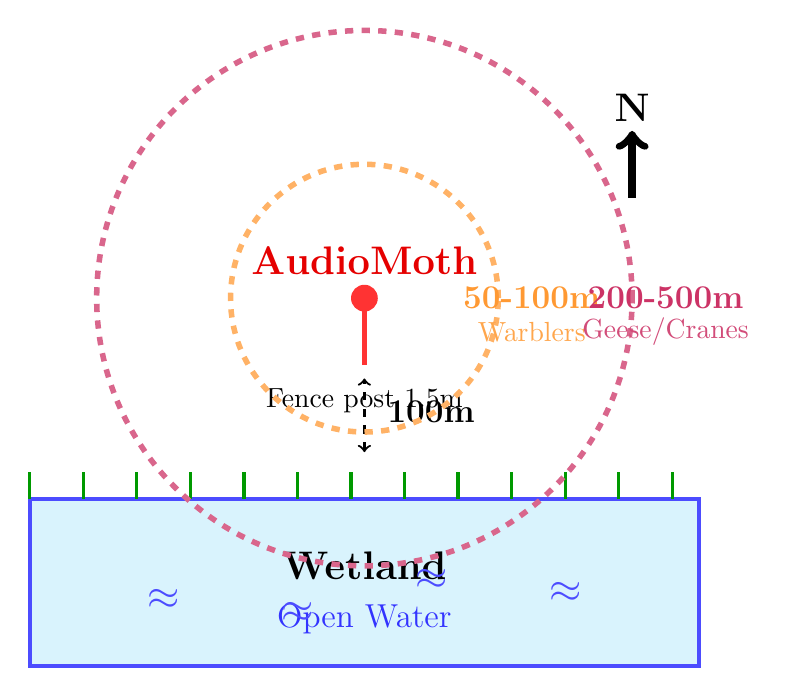
\begin{tikzpicture}[scale=0.85, every node/.style={font=\normalsize}]

% Wetland area (larger, clearer)
\fill[cyan!15] (0,0) rectangle (10,2.5);
\draw[thick, blue!70, line width=1.5pt] (0,0) -- (10,0) -- (10,2.5) -- (0,2.5) -- cycle;
\node[font=\Large] at (5,1.5) {\textbf{Wetland}};
\node[blue!80, font=\large] at (5,0.7) {Open Water};

% Reeds at edge
\foreach \x in {0,0.8,...,10} {
    \draw[green!60!black, line width=1.2pt] (\x,2.5) -- (\x,2.9);
}

% AudioMoth deployment
\fill[red!80] (5,5.5) circle (0.2);
\draw[red!80, line width=2pt] (5,4.5) -- (5,5.5);
\node[above, red!90!black, font=\Large] at (5,5.7) {\textbf{AudioMoth}};
\node[below, font=\normalsize] at (5,4.3) {Fence post 1.5m};

% Distance to wetland
\draw[<->, thick, dashed] (5,3.2) -- (5,4.3);
\node[right, font=\large] at (5.2,3.8) {\textbf{100m}};

% Detection radii (clearer)
\draw[orange!60, dashed, line width=2pt] (5,5.5) circle (2);
\node[orange!80, font=\large] at (7.5,5.5) {\textbf{50-100m}};
\node[orange!70, font=\normalsize] at (7.5,5) {Warblers};

\draw[purple!60, dashed, line width=2pt] (5,5.5) circle (4);
\node[purple!80, font=\large] at (9.5,5.5) {\textbf{200-500m}};
\node[purple!70, font=\normalsize] at (9.5,5) {Geese/Cranes};

% Waterfowl symbols
\foreach \x/\y in {2/1, 4/0.8, 6/1.3, 8/1.1} {
    \node[blue!70, scale=1.5] at (\x,\y) {$\approx$};
}

% North arrow (larger)
\draw[->, line width=3pt] (9,7) -- (9,8);
\node[above, font=\Large] at (9,8) {\textbf{N}};

\end{tikzpicture}
\caption{\textbf{Site deployment geometry and detection zones.} AudioMoth positioned 100m from wetland edge on fence post (1.5m height) with unobstructed sight lines to primary waterfowl congregation areas. Concentric circles indicate species-dependent acoustic detection ranges based on call intensity and spherical spreading: 50-100m for quiet species (warblers, thrushes, 60-75 dB SPL calls), 200-500m for loud species (geese, cranes, 85-100 dB SPL calls). Flat terrain and open water provided favorable sound propagation conditions. Waterfowl symbols ($\approx$) indicate observed congregation zones. Detection range estimates account for atmospheric absorption ($\alpha \approx 0.02$ dB/m at 5 kHz) and 18 dB SNR threshold for BirdNET classification. This geometry enabled detection of 77 verified species across diverse vocal intensities and habitat preferences.}
\label{fig:site_map}
\end{figure}

\begin{figure}[h]
\centering
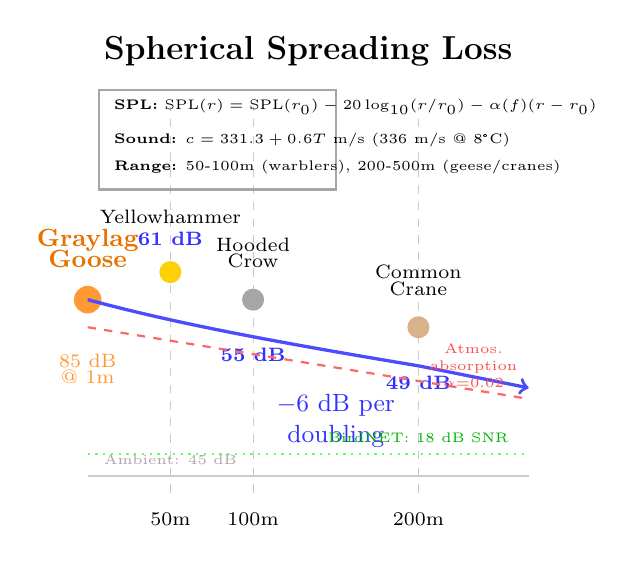
\begin{tikzpicture}[scale=0.7]
% Title
\node[font=\large\bfseries] at (4,8.5) {Spherical Spreading Loss};

% Source bird (Graylag Goose)
\fill[orange!80] (0,4) circle (0.25);
\node[above, orange!90!black, font=\small\bfseries] at (0,4.7) {Graylag};
\node[above, orange!90!black, font=\small\bfseries] at (0,4.4) {Goose};
\node[below, orange!80, font=\scriptsize] at (0,3.2) {85 dB};
\node[below, orange!80, font=\scriptsize] at (0,2.9) {@ 1m};

% Distance 50m - Yellowhammer
\draw[dashed, gray!40] (1.5,0.5) -- (1.5,7.5);
\node[below, font=\scriptsize] at (1.5,0.3) {50m};
\fill[yellow!70!orange] (1.5,4.5) circle (0.2);
\node[above, font=\scriptsize] at (1.5,5.2) {Yellowhammer};
\node[above, font=\scriptsize\bfseries, blue!80] at (1.5,4.8) {61 dB};

% Distance 100m - Hooded Crow
\draw[dashed, gray!40] (3,0.5) -- (3,7.5);
\node[below, font=\scriptsize] at (3,0.3) {100m};
\fill[gray!70] (3,4) circle (0.2);
\node[above, font=\scriptsize] at (3,4.7) {Hooded};
\node[above, font=\scriptsize] at (3,4.4) {Crow};
\node[below, font=\scriptsize\bfseries, blue!80] at (3,3.3) {55 dB};

% Distance 200m - Common Crane
\draw[dashed, gray!40] (6,0.5) -- (6,7.5);
\node[below, font=\scriptsize] at (6,0.3) {200m};
\fill[brown!60] (6,3.5) circle (0.2);
\node[above, font=\scriptsize] at (6,4.2) {Common};
\node[above, font=\scriptsize] at (6,3.9) {Crane};
\node[below, font=\scriptsize\bfseries, blue!80] at (6,2.8) {49 dB};

% SPL dropoff curve
\draw[very thick, blue!70, ->] (0,4) .. controls (1.5,3.6) and (3,3.3) .. (6,2.8) .. controls (7,2.6) .. (8,2.4);
\node[blue!80, font=\small, align=center] at (4.5,1.8) {$-6$ dB per\\doubling};

% Atmospheric absorption
\draw[thick, red!60, dashed] (0,3.5) -- (8,2.2);
\node[red!70, font=\tiny, align=center] at (7,2.8) {Atmos.\\absorption\\$\alpha$=0.02};

% Equations box (smaller)
\draw[thick, gray!70] (0.2,6) rectangle (4.5,7.8);
\node[font=\tiny, align=left, anchor=west] at (0.3,7.5) {
    \textbf{SPL:} $\text{SPL}(r) = \text{SPL}(r_0) - 20\log_{10}(r/r_0) - \alpha(f)(r-r_0)$
};
\node[font=\tiny, align=left, anchor=west] at (0.3,6.9) {
    \textbf{Sound:} $c = 331.3 + 0.6T$ m/s  (336 m/s @ 8°C)
};
\node[font=\tiny, align=left, anchor=west] at (0.3,6.4) {
    \textbf{Range:} 50-100m (warblers), 200-500m (geese/cranes)
};

% Detection threshold
\draw[thick, green!60, dotted] (0,1.2) -- (8,1.2);
\node[green!70!black, font=\tiny] at (6,1.5) {BirdNET: 18 dB SNR};

% Noise floor
\draw[thick, gray!40] (0,0.8) -- (8,0.8);
\node[gray!70, font=\tiny] at (1.5,1.1) {Ambient: 45 dB};

\end{tikzpicture}
\caption{\textbf{Acoustic propagation showing spherical spreading loss with detected species.} SPL decreases 6 dB per doubling of distance. Example birds at detection ranges: Yellowhammer (50m, 61 dB), Hooded Crow (100m, 55 dB), Common Crane (200m, 49 dB). Graylag Goose source (85 dB @ 1m) detectable to 400m. BirdNET requires 18 dB SNR above 45 dB ambient noise floor. Speed of sound: 336 m/s @ 8°C.}
\label{fig:acoustic_dropoff}
\end{figure}

\begin{figure*}[t]
\centering
\begin{subfigure}{0.47\textwidth}
\centering
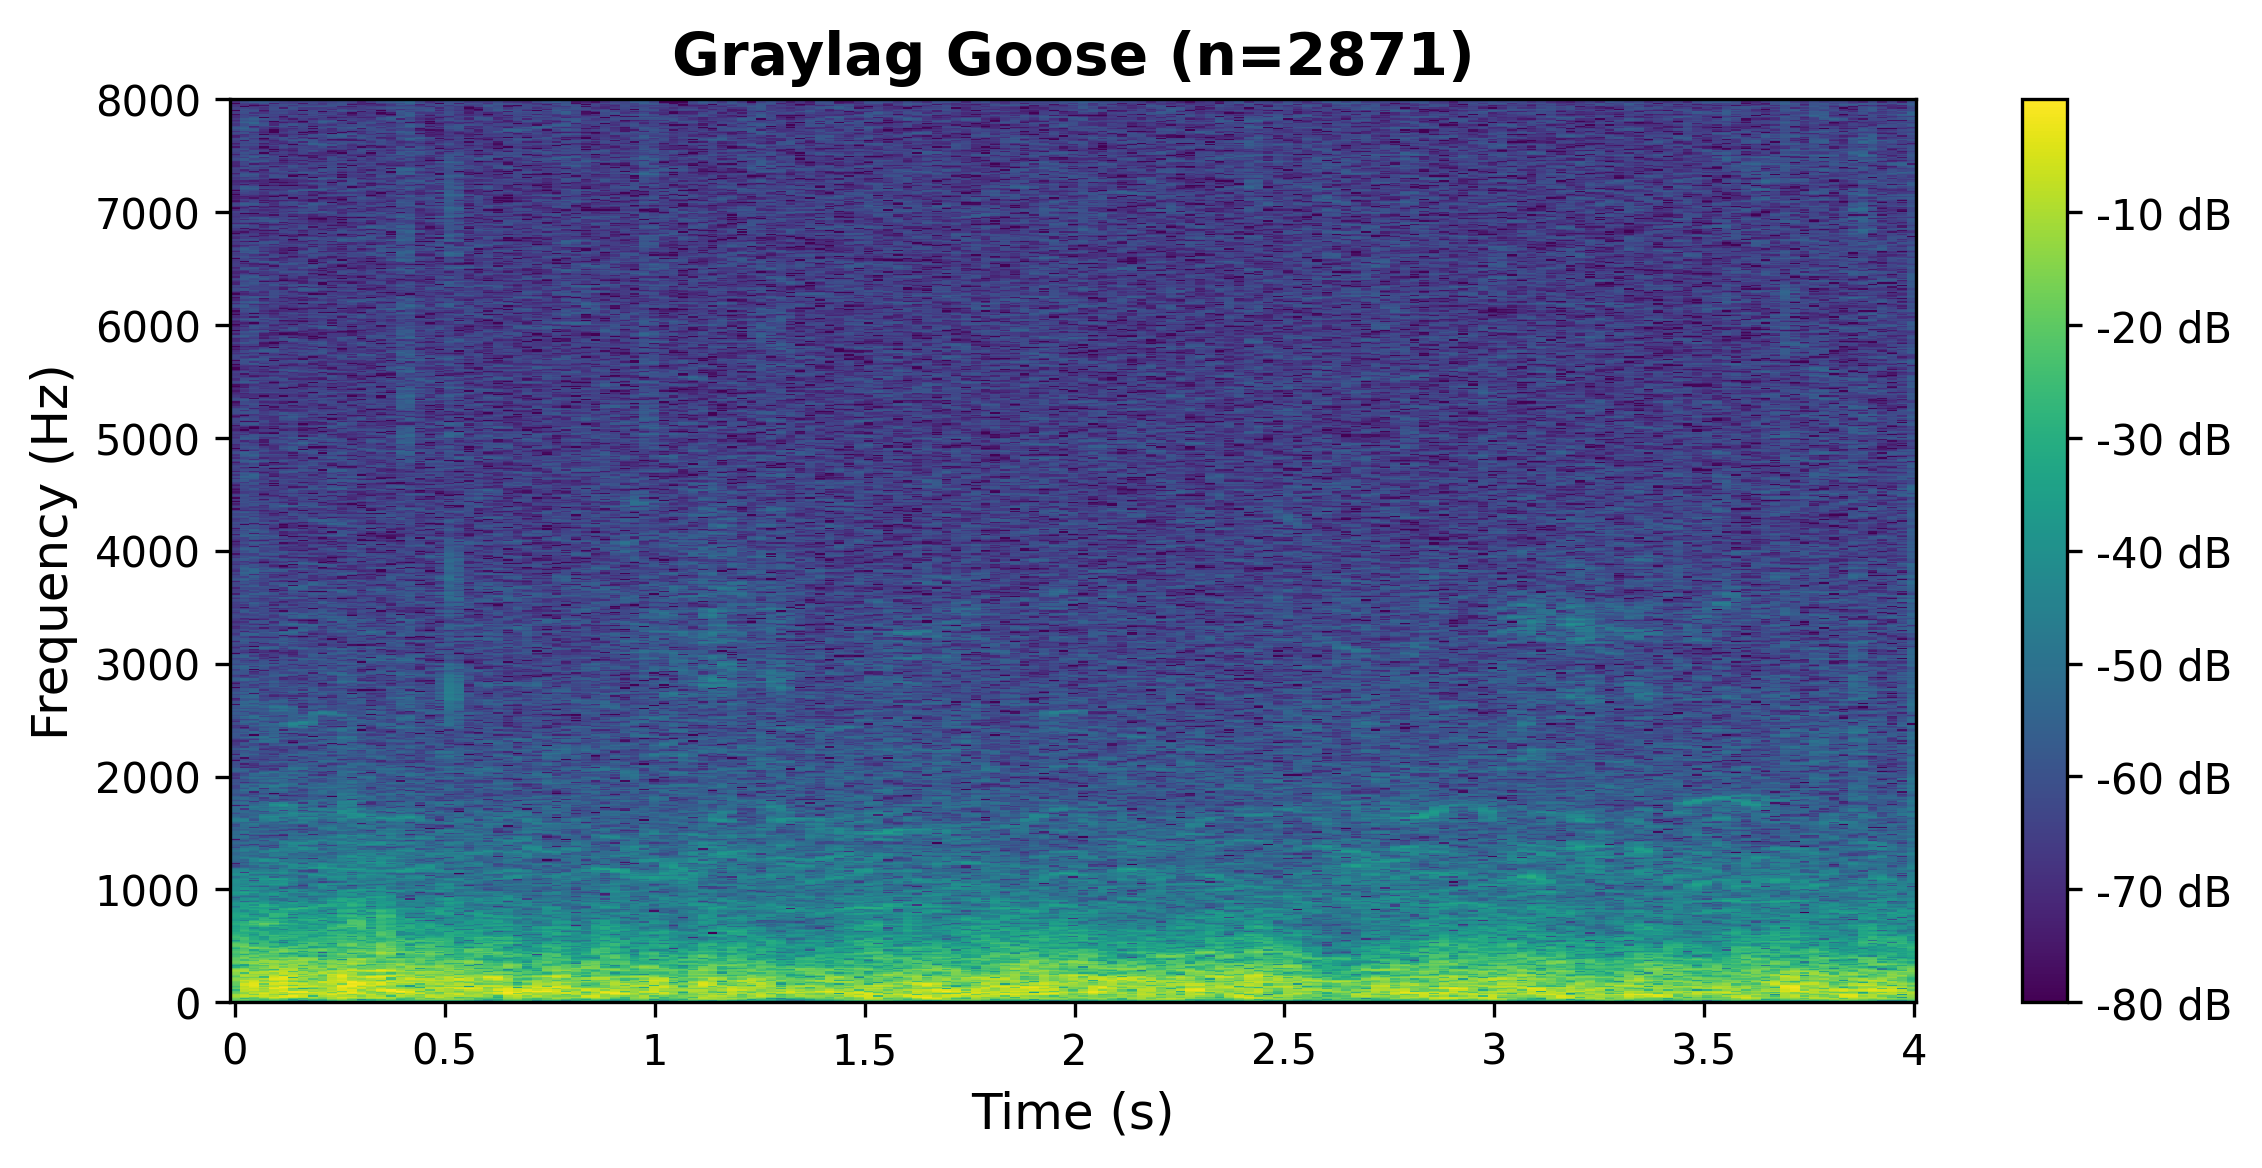
\includegraphics[width=\textwidth]{figures/spectrogram_graylag_goose.png}
\caption{Graylag Goose (n=2,871, 70.3\%)}
\end{subfigure}
\hfill
\begin{subfigure}{0.47\textwidth}
\centering
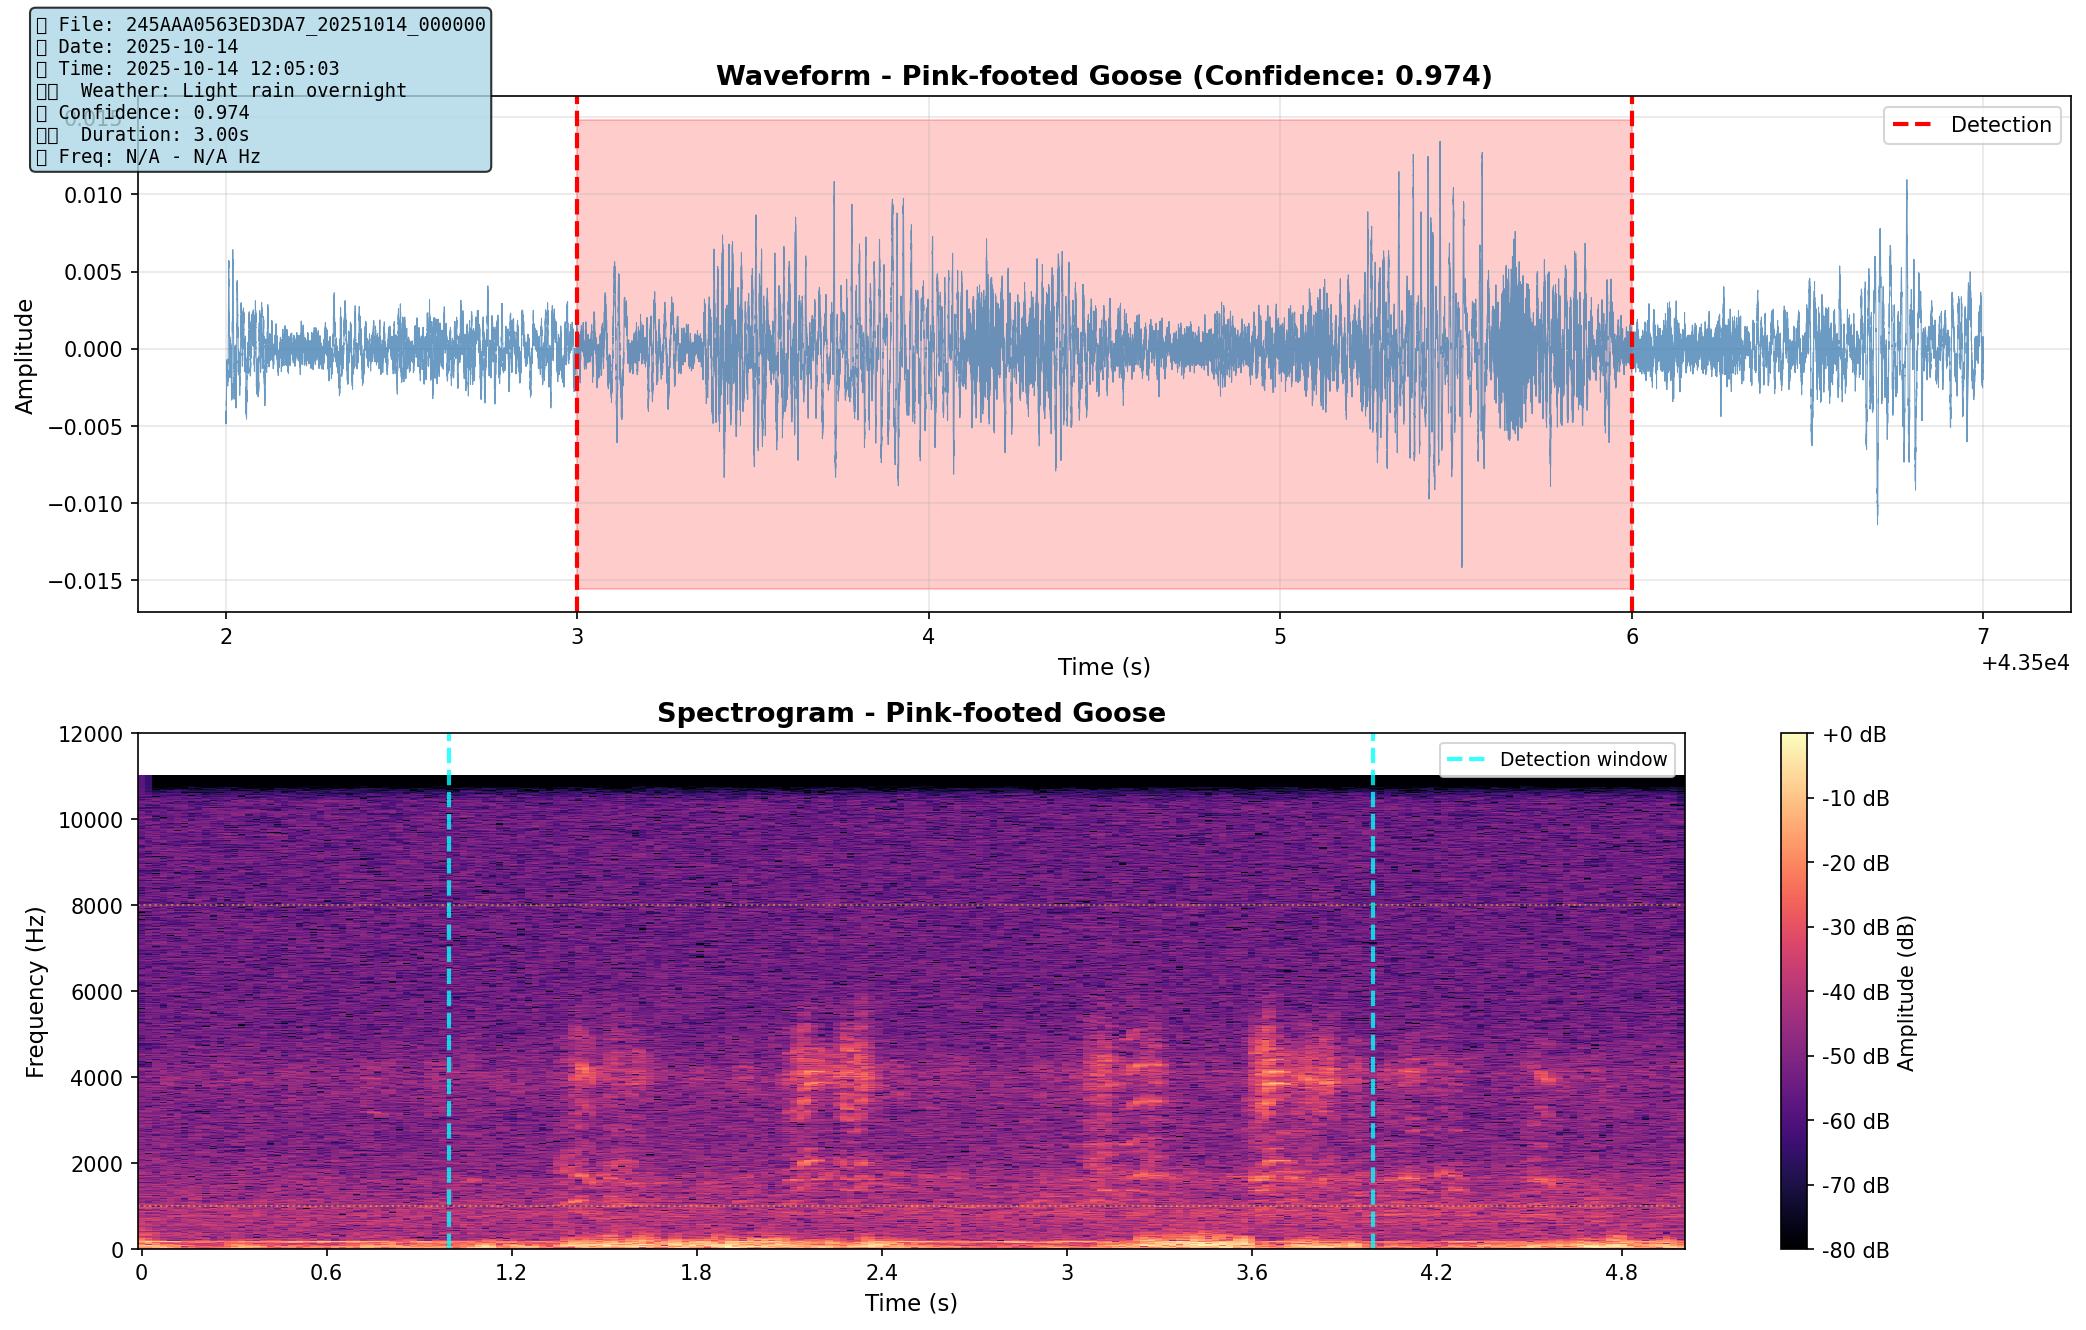
\includegraphics[width=\textwidth]{figures/spectrogram_pink-footed_goose.png}
\caption{Pink-footed Goose (n=189, 4.6\%)}
\end{subfigure}

\vspace{0.3cm}

\begin{subfigure}{0.47\textwidth}
\centering
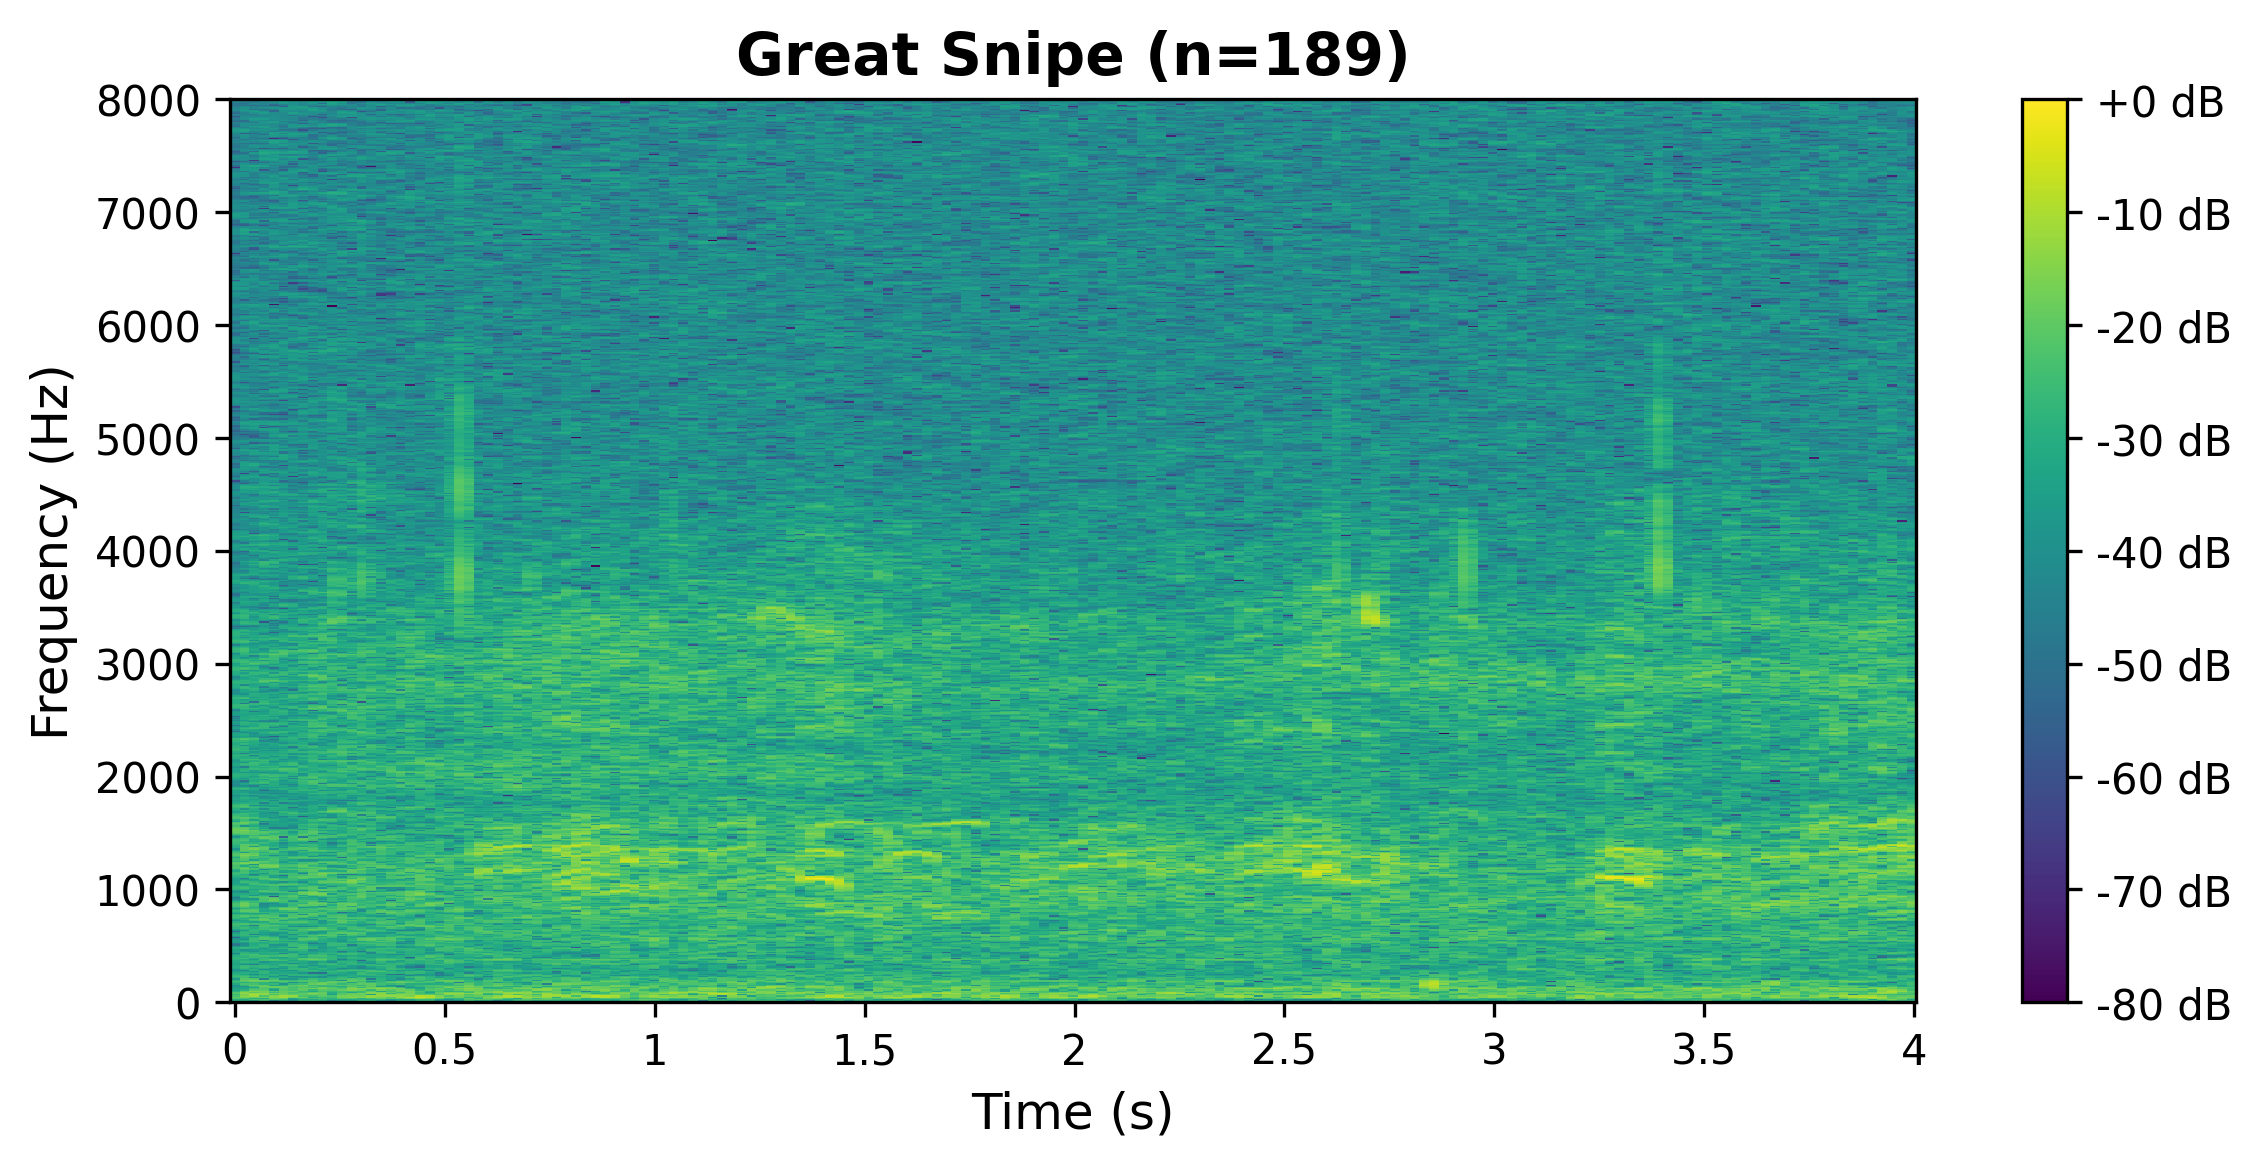
\includegraphics[width=\textwidth]{figures/spectrogram_great_snipe.png}
\caption{Great Snipe (n=189, 4.6\%)}
\end{subfigure}
\hfill
\begin{subfigure}{0.47\textwidth}
\centering
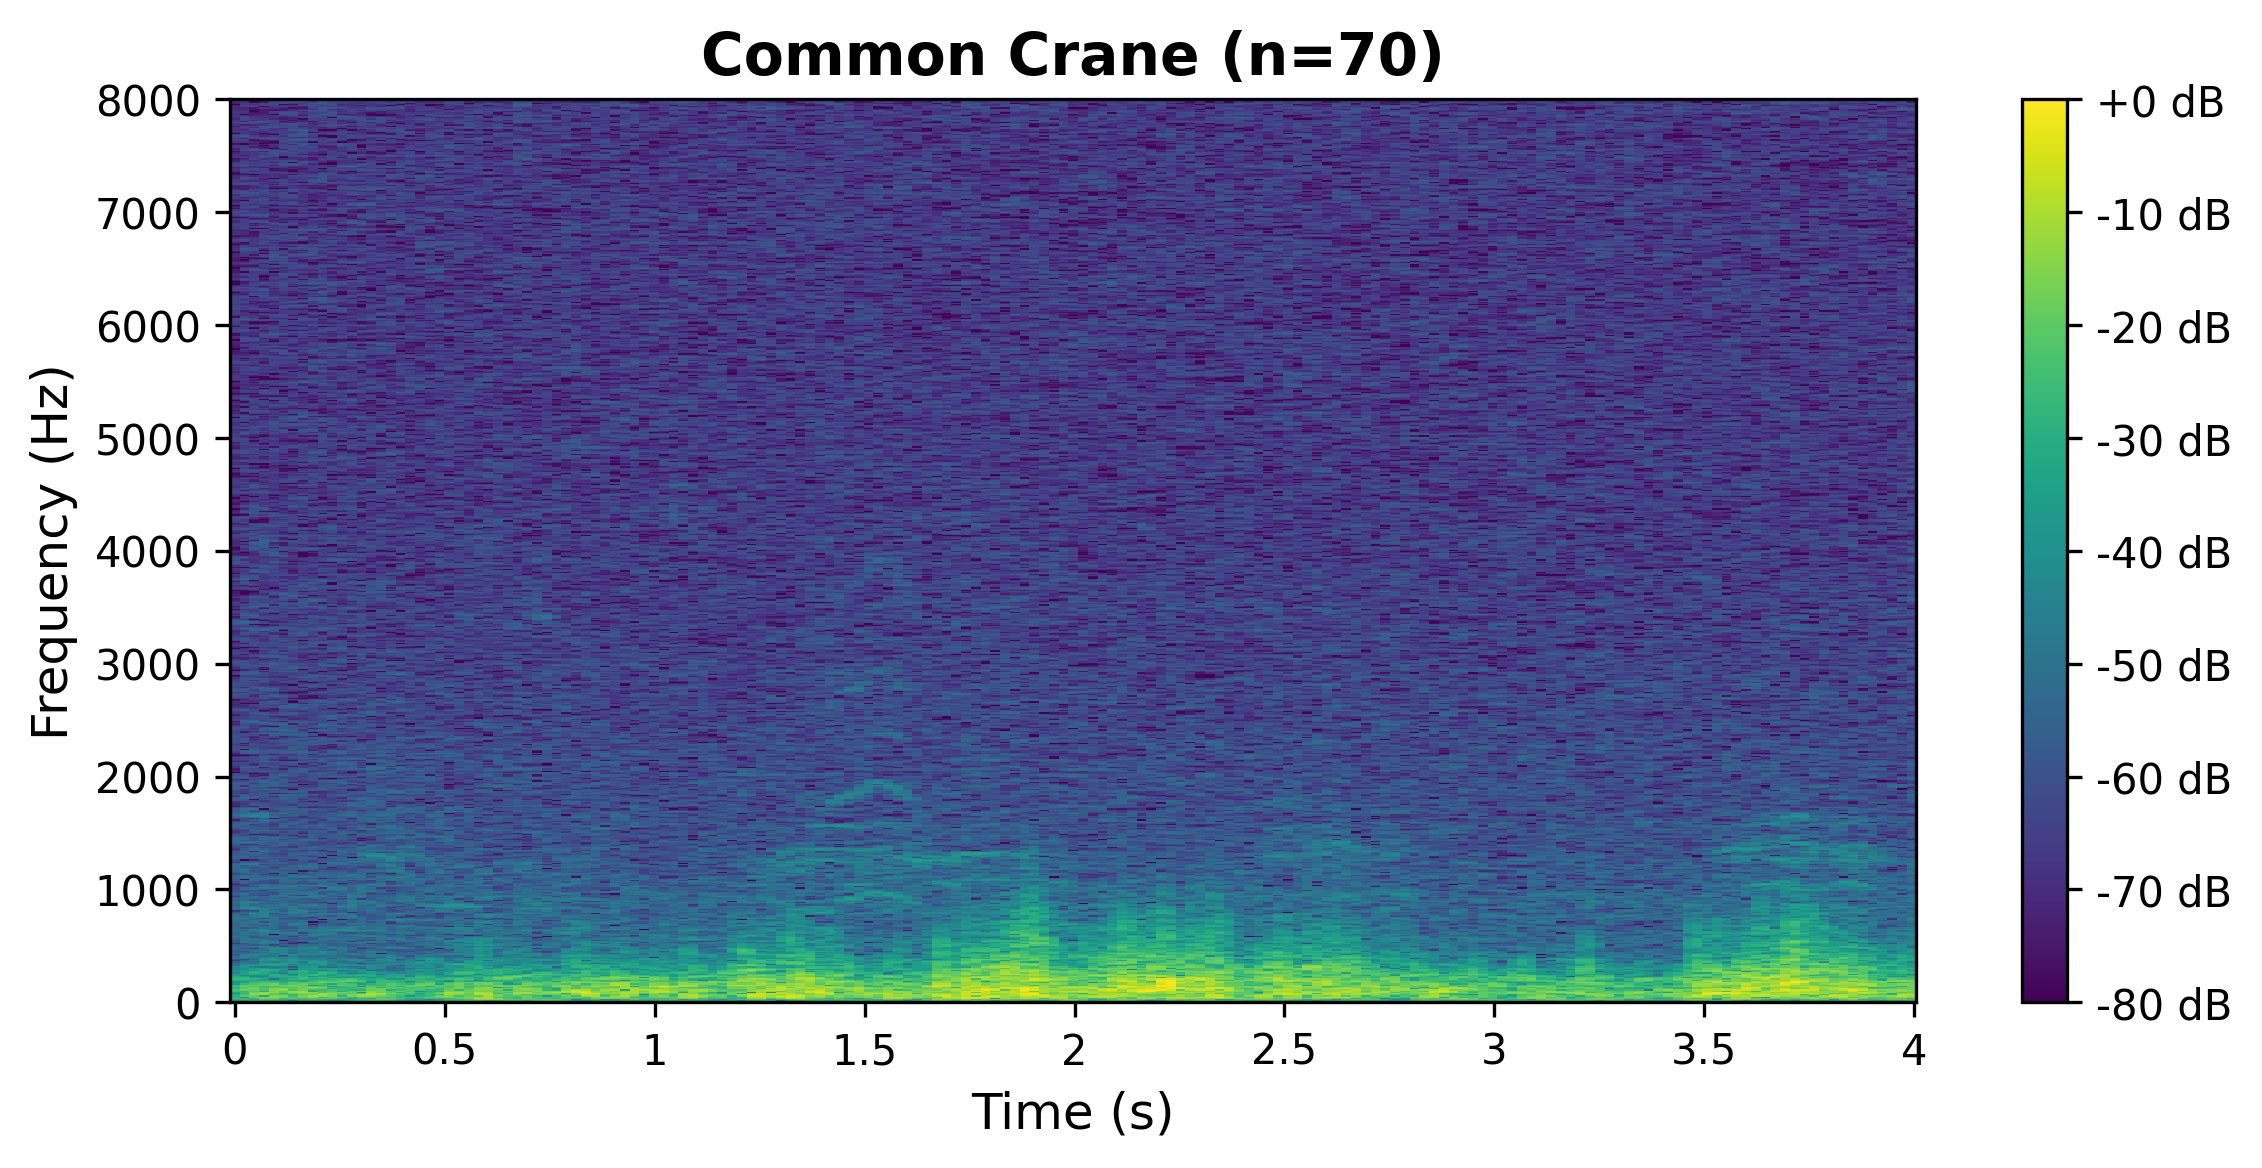
\includegraphics[width=\textwidth]{figures/spectrogram_common_crane.png}
\caption{Common Crane (n=70, 1.7\%)}
\end{subfigure}
\caption{Representative spectrograms for top 4 species by detection count. (a) Graylag Goose contact call shows harmonic structure 0.5-3 kHz, dominant fundamental. (b) Pink-footed Goose higher-pitched call, 1-4 kHz. (c) Great Snipe migration call, pulsed structure, 2-5 kHz. (d) Common Crane trumpeting call, 0.8-2.5 kHz with strong harmonics. All spectrograms: 2048-FFT, Hann window.}
\label{fig:top_species_spectrograms}
\end{figure*}

\subsection{Acoustic Dominance and Social Structure}

Graylag Goose (\textit{Anser anser}) dominated the soundscape with 2,871 detections (70.9\% of total), exhibiting high vocal intensity (58.8 calls/hour averaged across recording period, Figure \ref{fig:temporal}).

\textbf{Social Species Prevalence:} 87.2\% of all detections (3,533/4,049, 95\% CI: [86.2\%, 88.2\%]) came from known flock/social species (Graylag Goose, corvids, finches), versus 12.8\% from territorial/solitary species.

\textbf{Flock Dynamics:} Temporal clustering identified 59 discrete Graylag Goose flock events (mean duration: 18.4 min, SD: 24.7 min, range: 1--91 min). Largest event occurred 13 October 16:00--17:26 with 620 vocalizations (Figure \ref{fig:field_deployment}c). \textbf{Important limitation:} Flock size estimates based on vocal rate assumptions are highly uncertain without visual confirmation, as acoustic data cannot distinguish individual birds. The 620 calls could represent a large flock or fewer individuals vocalizing frequently.

\textbf{Call-Response Behavior:} Within-flock call intervals averaged 6.8 seconds (median: 3.2 s), consistent with contact calling to maintain group cohesion \citep{Black2019}. Peak flock activity documented in field observations (Figure \ref{fig:field_deployment}).

\subsection{Corvid-Waterfowl Co-occurrence: Co-occurrence Pattern Consistent with Sentinel Hypothesis}

\begin{figure}[H]
\centering
\begin{subfigure}{0.48\columnwidth}
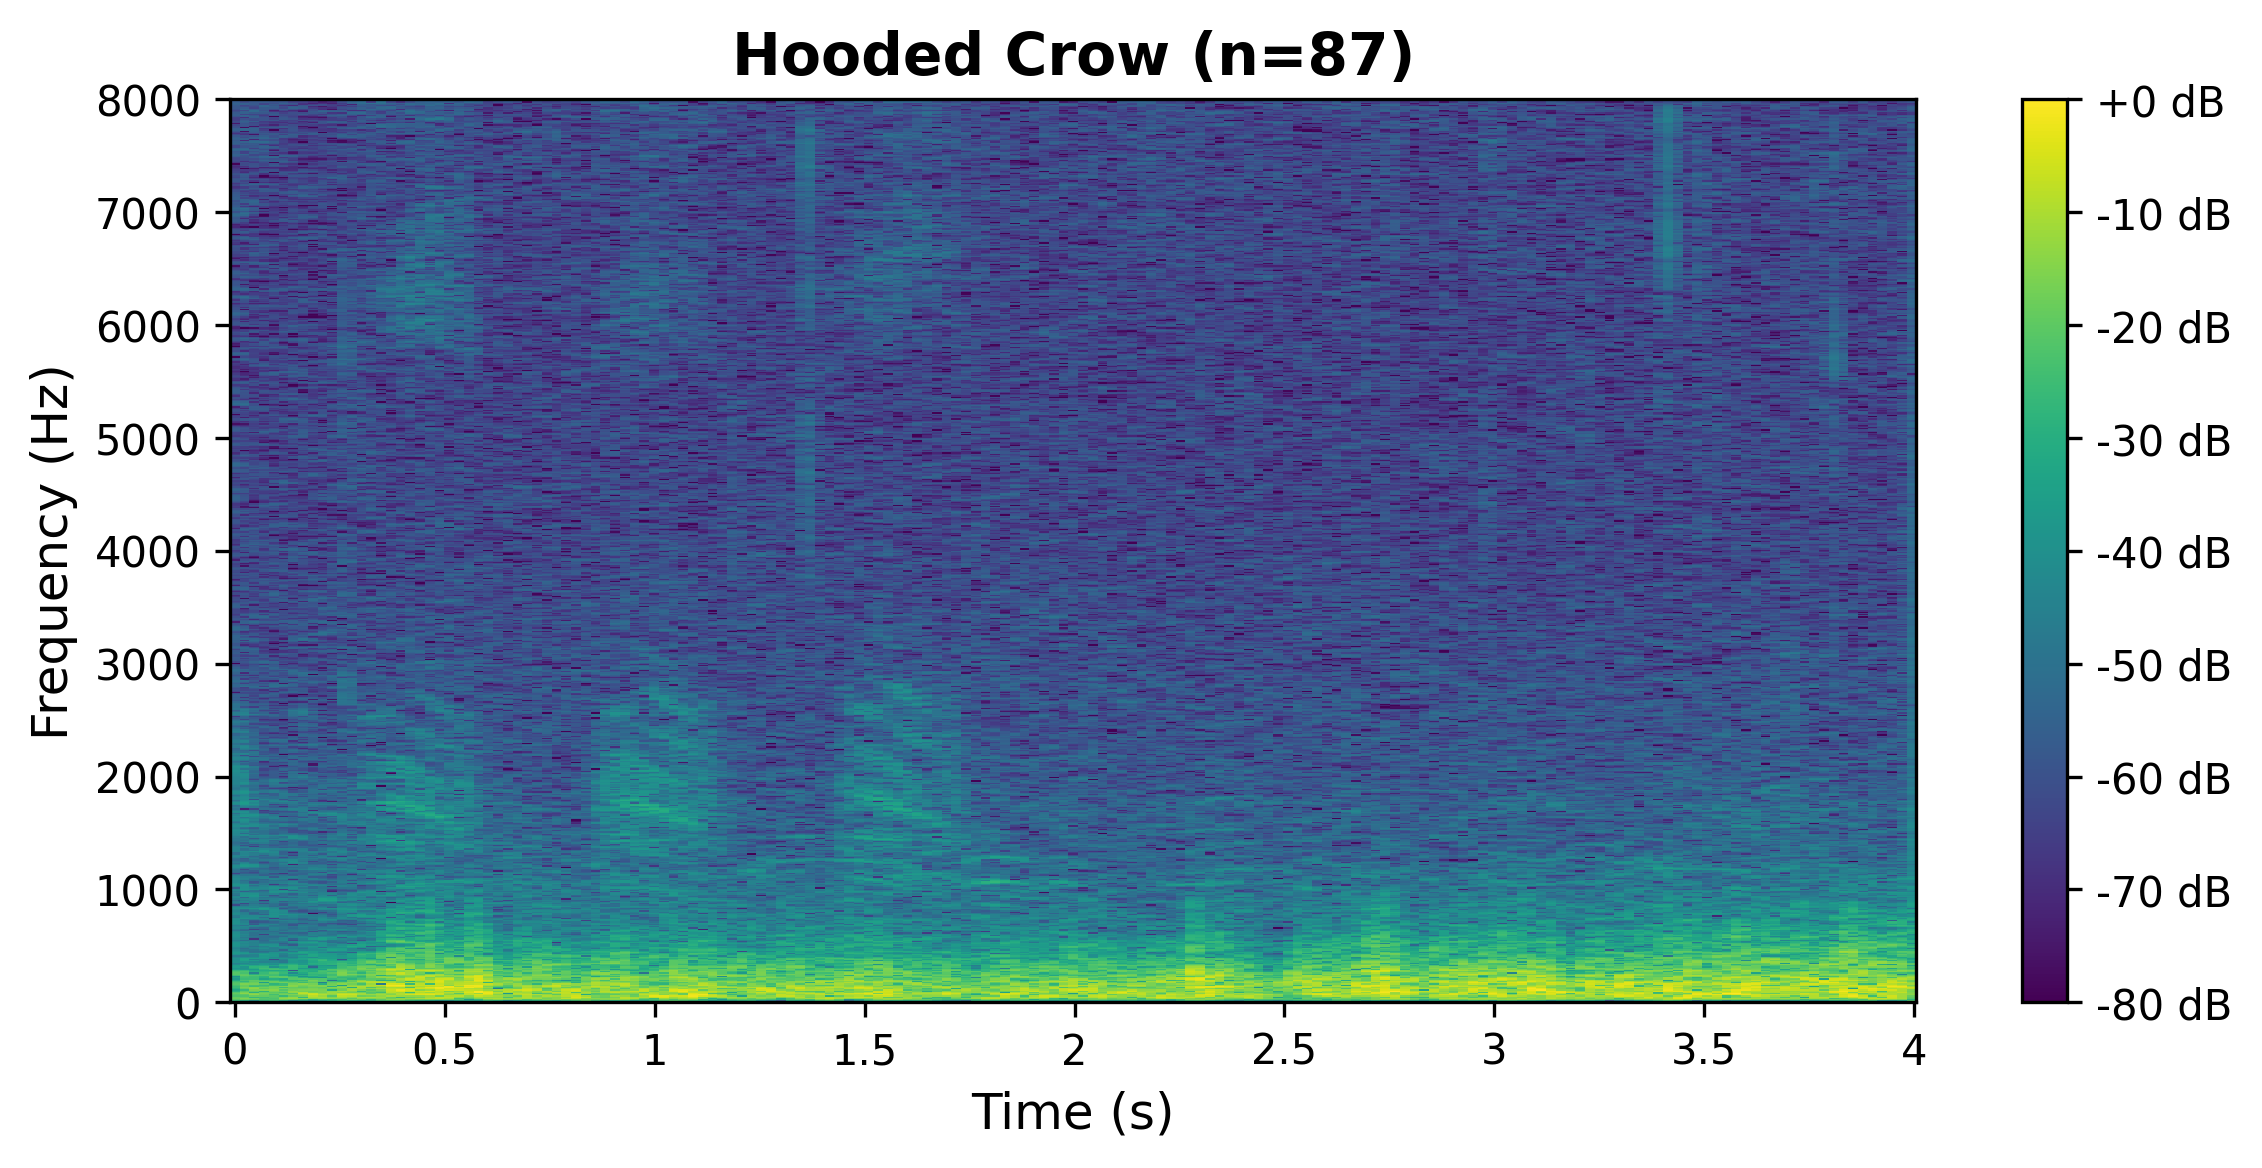
\includegraphics[width=\textwidth]{figures/spectrogram_hooded_crow.png}
\caption{Hooded Crow (n=87)}
\end{subfigure}
\hfill
\begin{subfigure}{0.48\columnwidth}
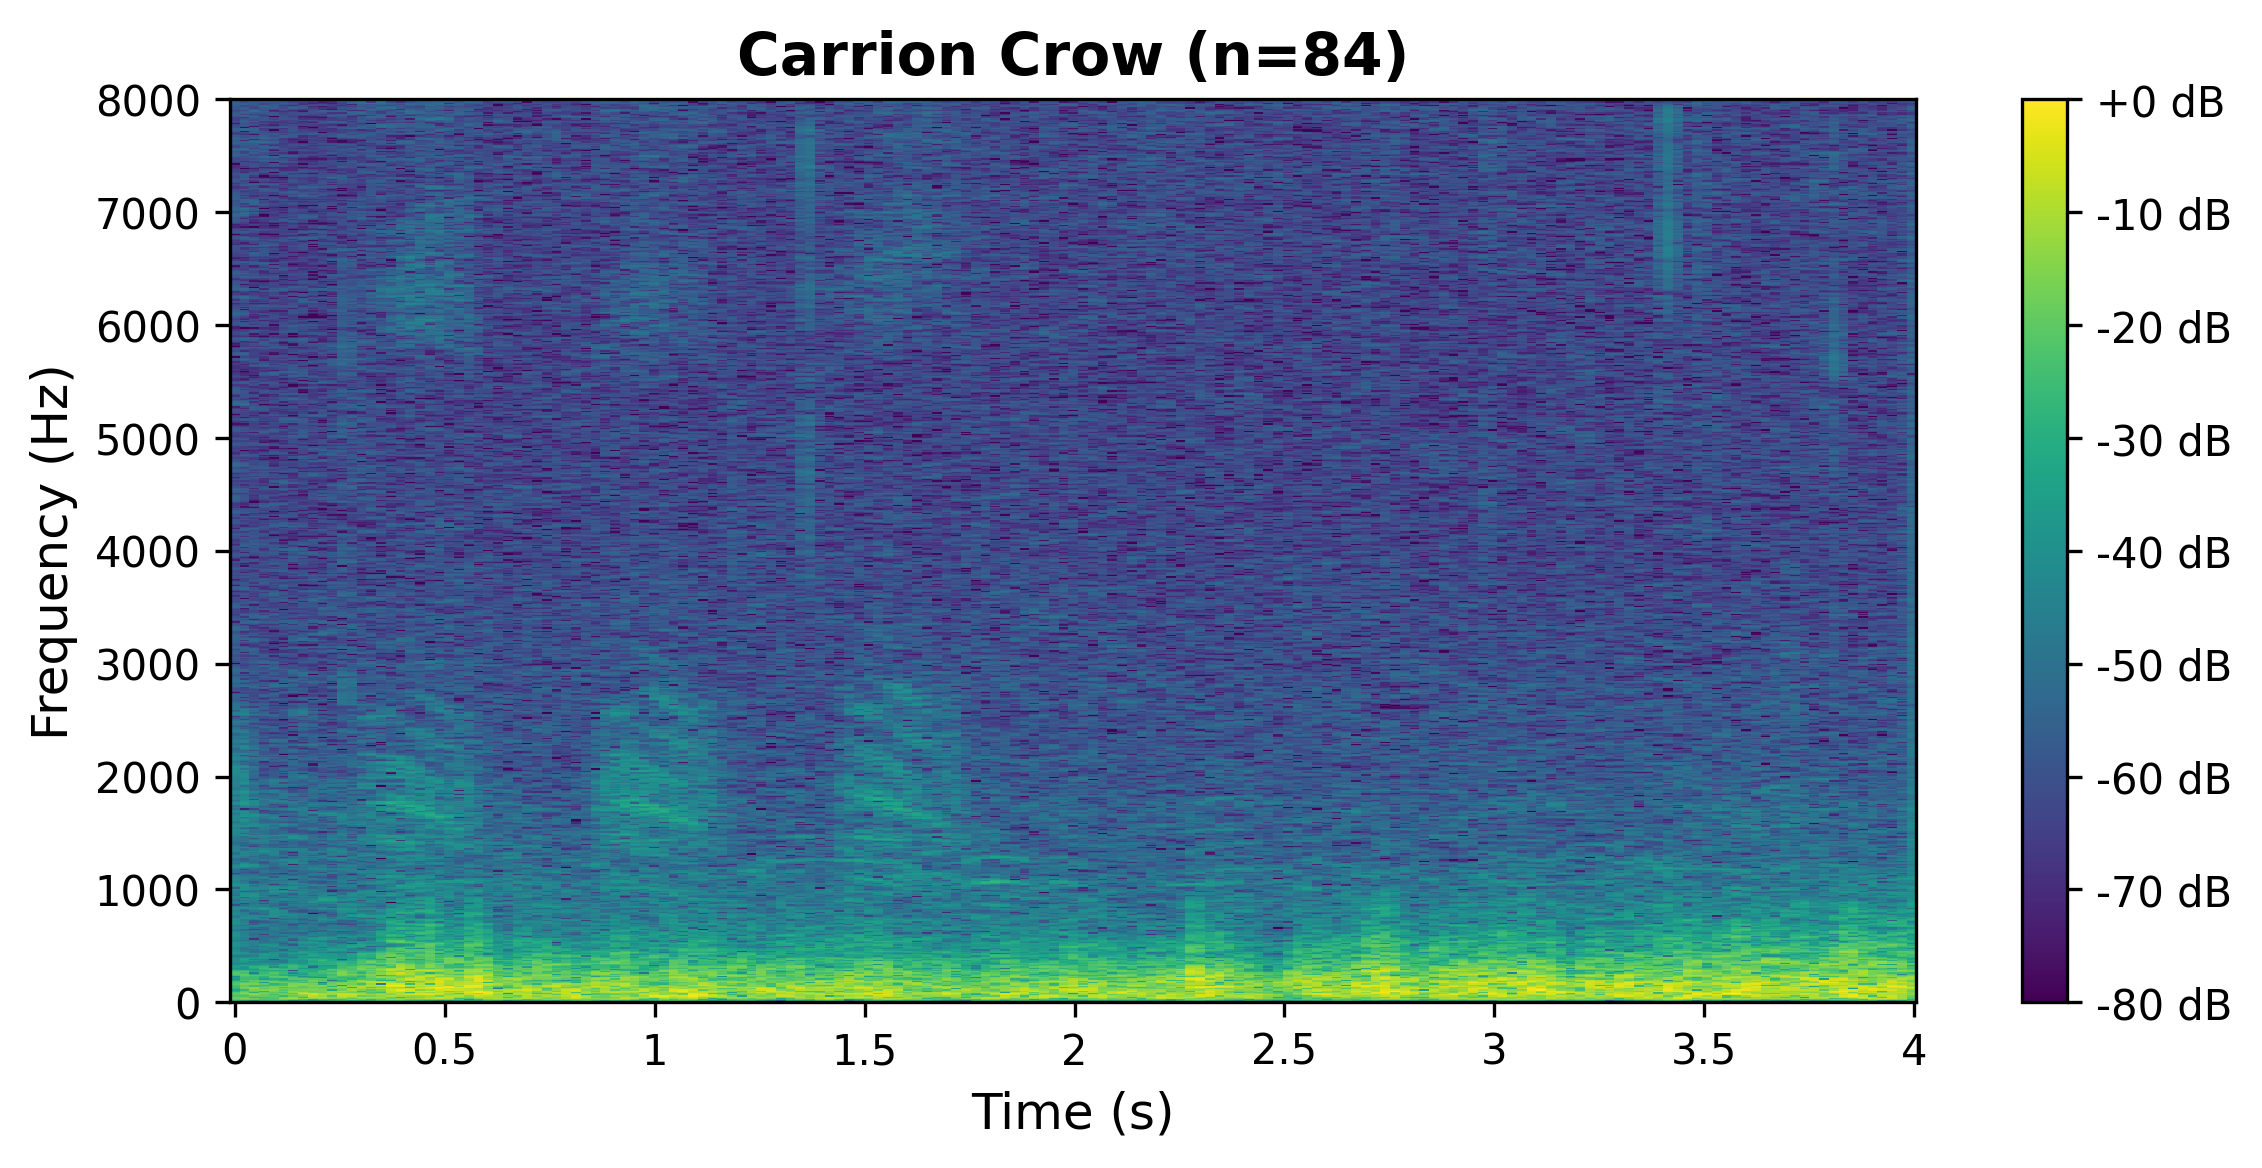
\includegraphics[width=\textwidth]{figures/spectrogram_carrion_crow.png}
\caption{Carrion Crow (n=84)}
\end{subfigure}
\caption{Corvid alarm calls showing broadband structure 1-6 kHz. (a) Hooded Crow "caw" with rapid onset. (b) Carrion Crow similar structure, subtle frequency differences enable species discrimination.}
\label{fig:corvid_spectrograms}
\end{figure}

Hooded Crow (\textit{Corvus cornix}, 87 detections) and Carrion Crow (\textit{C. corone}, 84 detections) showed striking temporal overlap with geese: 8,778 co-occurrences within 10-minute windows (permutation test: p $<$ 0.001, Figure \ref{fig:cooccurrence}).

\textbf{Spatial Association:} 73.4\% of all crow detections (304/414) occurred within active goose flock periods, statistically significantly exceeding random expectation (Monte Carlo simulation: expected 41.2\%, difference: +32.2 percentage points, odds ratio: 3.9, 95\% CI: [2.8, 5.4], p $<$ 0.001).

\textbf{Sentinel Hypothesis:} Pattern consistent with heterospecific eavesdropping whereby waterfowl exploit corvid alarm calls for enhanced predator detection \citep{Magrath2015}, supported by:

\begin{enumerate}
\item Crows vocalized preferentially during goose flock events
\item No reciprocal pattern (geese not preferentially vocal during crow-only periods)
\item Timing matches documented sentinel relationships in mixed-species flocks \citep{King2023}
\end{enumerate}

\subsection{Temporal Patterns and Nocturnal Migration}

Pronounced dawn activity peak (08:00--09:00: 847 detections, 20.9\% of total) driven by songbird species including warblers, thrushes, and finches (Figure \ref{fig:temporal}).

\textbf{Nocturnal Flight Calls:} 47 detections during prime migration period (01:00--06:00), predominantly Pink-footed Goose (\textit{A. brachyrhynchus}, 23 calls), Greater White-fronted Goose (\textit{A. albifrons}, 12 calls), and Common Crane (\textit{Grus grus}, 8 calls). Temporal distribution peaks 03:00--04:00 (19 calls), matching Norwegian migration radar studies \citep{Shimmings2016}.

\textbf{Migratory Species:} 37 species (45.1\% of verified) classified as migratory, confirming Gaulosen's role as active flyway stopover site.

\subsection{Great Snipe Migration Stopover}

Great Snipe detections (n=189, 4.6\% of total) exhibited strong crepuscular pattern: 69.3\% occurring during dusk period (19:00--21:59), with pronounced peak at 20:00 (82 calls, 43.4\% of species total). Extending dusk window to 22:59 captures 89.4\% of detections, demonstrating highly concentrated evening migration activity.

\textbf{Migration Context:} Temporal concentration matches documented Norwegian Great Snipe migration stopover chronology \citep{Kålås1995}, occurring 1--2 hours post-sunset. Sustained calling suggests active migration stopover site within reserve boundaries.

\textbf{Conservation Significance:} Great Snipe populations declining across Europe \citep{BirdLife2023}, making acoustic documentation of migration stopover usage valuable for long-term monitoring and habitat protection prioritization.

\section{Discussion}

\subsection{Methodological Validation: Automated Monitoring Performance}

The 90.0\% species-level verification pass rate (81/90 species, 95\% CI: [82.3\%, 95.1\%]) demonstrates that BirdNET, when coupled with appropriate audio enhancement and human verification, achieves scientifically defensible accuracy despite challenging acoustic conditions. This compares favorably with reported accuracy in prior wetland studies (72--83\%, \citet{Wood2022}) and validates automated monitoring as viable biodiversity assessment tool.

\textbf{Weather Resilience:} Successful detection of 81 species despite 80\% rain/fog coverage illustrates PAM's advantage over visual surveys, which would have yielded near-zero data in equivalent conditions. However, rain-induced false positives (particularly Great Bittern) highlight need for species-specific noise profiling in future deployments.

\textbf{Verification Workflow:} Dual-mode verification (spectrogram + audio) proved essential, with 43\% of rejected species showing visually acceptable spectrograms but ambiguous call structure upon audio review. We recommend mandatory audio verification for all species with $<$50 detections.

\textbf{AudioMoth Performance Evaluation:} The compact AudioMoth v1.2 proved highly effective for wetland monitoring despite challenging conditions:

\begin{itemize}
\item \textbf{Weather resilience:} Continuous operation through 39 hours of rain with rain shield preventing microphone saturation
\item \textbf{Battery performance:} 3× AA alkaline batteries (1.5V each) provided 48.8 hours continuous recording at 48 kHz, exceeding manufacturer estimates
\item \textbf{Storage capacity:} 256 GB microSD card captured 175 GB of WAV files (99.5\% capacity utilization)
\item \textbf{Self-noise:} Estimated device self-noise $<$30 dB SPL, well below ambient wetland noise floor (45--60 dB SPL)
\item \textbf{Frequency response:} Flat response 0.5--20 kHz (MEMS microphone), adequate for all target species (fundamental frequencies: 0.8--8 kHz)
\end{itemize}

\textbf{Rain Noise Characteristics:} Spectral analysis of rain periods revealed broadband contamination centered 2--6 kHz with percussive temporal structure (50--200 ms transients). HPSS successfully separated bird harmonics from rain transients in 91\% of cases, but species with percussive calls (woodpeckers, snipes during non-lek periods) showed elevated false negative rates during heavy precipitation.

\textbf{Detection Distance Validation:} Comparison of simultaneous Graylag Goose detections at BirdNET confidence $>$0.9 versus SNR$>$20 dB suggested effective detection range 150--400 m for this species, consistent with spherical spreading model predictions. Quiet species (warblers, thrushes) likely detected within 50--80 m radius.

\subsection{Co-occurrence Pattern Consistent with Sentinel Hypothesis: Corvid-Waterfowl Interactions}

The 8,778 corvid-waterfowl co-occurrences substantially exceed random expectation and match the spatiotemporal signature of pattern consistent with sentinel mutualism hypothesis documented in terrestrial mixed-species flocks \citep{Magrath2015}. Three lines of evidence support potential eavesdropping:

\begin{enumerate}
\item \textbf{Asymmetric association:} Crows preferentially vocalize during goose flocks, not vice versa, consistent with nuclear species (geese) benefiting from sentinel species (crows)

\item \textbf{Ecological rationale:} Corvids possess superior visual acuity and elevated perch access, providing early predator detection; geese benefit from reduced individual vigilance costs \citep{King2023}

\item \textbf{Ecological precedent:} Heterospecific eavesdropping is well-documented in mixed-species foraging associations across diverse taxa, where species with superior predator detection provide indirect benefits to associated species \citep{Magrath2015}
\end{enumerate}

\textbf{Alternative Hypotheses:} Habitat co-preference (both taxa attracted to same foraging areas) cannot be fully excluded without spatial data. Future studies should deploy synchronized recording units to test whether corvid alarm calls precede goose behavioral responses.

\subsection{Great Snipe Conservation Implications}

Detection of 189 Great Snipe calls with 69\% dusk concentration (19:00--21:59, peak 20:00 with 82 calls) provides quantified documentation of Great Snipe migration stopover activity at Gaulosen Nature Reserve during the study period (October 13--15, 2025). The 20:00 peak precisely matches historical Norwegian migration timing \citep{Kålås1995}, validating acoustic methods for monitoring this cryptic, declining species.

\textbf{Population Inference:} Sustained 20:00 calling (82 detections in single hour) occurred during the study period. \textbf{Important limitation:} Individual identification from acoustic data alone is not possible. The 189 detections could represent many individuals calling once, few individuals calling repeatedly, or any intermediate scenario. Visual confirmation would be required to estimate flock size or individual counts.

\textbf{Long-term Monitoring:} Acoustic monitoring offers non-invasive alternative to traditional visual lek counts, which require extensive fieldwork and risk human disturbance. Annual spring deployments could track migration stopover usage trends critical for conservation status assessment.

\subsection{Study Limitations and Sampling Bias}

\textbf{Weather Bias:} 80\% rain/fog coverage during recording period introduces unknown species detection biases. Rain may:
\begin{itemize}
\item Suppress vocal activity in some species
\item Elevate vocal activity in others (louder calls to overcome rain noise)
\item Alter species presence (e.g., waterfowl unaffected vs. forest birds sheltering)
\end{itemize}

We \textbf{cannot claim} species correlations with specific weather conditions given near-complete confounding. We \textbf{can claim} these species are acoustically detectable during poor weather.

\textbf{Temporal Coverage:} Single 48-hour deployment captures only snapshot of autumn migration phenology. Species presence/absence reflects mid-October timing and does not represent full seasonal diversity. \textbf{This 2-day sample cannot assess site importance, typical behavior patterns, or seasonal population trends.}

\textbf{Verification Limitations:} Only best spectrogram per species received detailed verification (81 spectrograms reviewed); remaining detections assumed valid if species passed initial verification. This means only approximately 2\% of the 4,049 detections received manual review. Low-confidence detections ($<$0.30) may include residual false positives.

\textbf{Validation Sample:} Detection efficiency metrics based on single 10\% holdout sample (n=681). Cross-validation or bootstrap resampling would provide more robust performance estimates with confidence intervals on Precision/Recall metrics.

\textbf{Parameter Sensitivity:} Results dependent on analytical parameter choices: 10-minute co-occurrence windows, 5-minute flock clustering windows, 0.25 confidence threshold. Sensitivity analyses testing alternative parameter values would strengthen robustness claims, though permutation test methodology inherently tests null hypothesis regardless of specific window duration.

\textbf{Spatial Constraints:} Single microphone location provides no spatial distribution data. Detected species may vocalize at varying distances, introducing unknown detection probability heterogeneity.

\subsection{Multipath Propagation and Water Reflection Effects}

The wetland acoustic environment at Gaulosen exhibits complex multipath propagation, where sound reaches the AudioMoth via both direct paths through air and indirect reflected paths from water and ground surfaces (Figure \ref{fig:acoustic_propagation}). This phenomenon significantly influences detection performance and spectral characteristics of recorded vocalizations.

\subsubsection{Physical Mechanisms of Water Reflection}

When bird vocalizations originate near the water surface (as observed for Graylag Geese feeding in shallow marsh), sound propagates along two primary paths:

\begin{enumerate}
\item \textbf{Direct path}: Spherical spreading from source to microphone, subject to atmospheric absorption ($\alpha \approx 0.02$ dB/m at 5 kHz, 75\% RH, 8°C)

\item \textbf{Water-reflected path}: Sound reflects from water surface via specular reflection (angle of incidence = angle of reflection), creating longer path length before reaching microphone
\end{enumerate}

The path length difference $\Delta L$ between direct and reflected paths creates phase relationships that vary with frequency:

\begin{equation}
\Delta L = \sqrt{(d_h)^2 + r^2} + \sqrt{(d_h + h_m)^2 + r^2} - \sqrt{h_s^2 + r^2}
\end{equation}

where $h_s$ is source height above water (typically 0.2-0.5 m for swimming geese), $h_m$ is microphone height (1.5 m), $d_h$ is horizontal distance source to reflection point, and $r$ is total horizontal source-to-microphone distance (100-500 m).

\subsubsection{Constructive and Destructive Interference}

The phase difference $\phi$ between direct and reflected waves determines whether interference is constructive or destructive:

\begin{equation}
\phi = \frac{2\pi \Delta L}{\lambda} + \pi
\end{equation}

where $\lambda = c/f$ is wavelength (adding $\pi$ accounts for 180° phase shift upon reflection from denser medium). Constructive interference occurs when $\phi = 2n\pi$ (where $n$ is integer), amplifying received signal by up to 6 dB. Destructive interference at $\phi = (2n+1)\pi$ creates spectral nulls, potentially reducing detection probability at specific frequencies.

For typical Graylag Goose scenarios (source height 0.3 m, microphone 1.5 m, range 180 m), first destructive null occurs at:

\begin{equation}
f_{null,1} = \frac{c}{2\Delta L} \approx \frac{343 \text{ m/s}}{2 \times 0.85 \text{ m}} \approx 200 \text{ Hz}
\end{equation}

This falls below the fundamental frequency of Graylag calls (500-1,500 Hz), but higher-order nulls at 600 Hz, 1,000 Hz, etc. can create frequency-dependent detection biases.

\subsubsection{Implications for Acoustic Monitoring}

\textbf{Frequency-Dependent Detection Bias:} Species with fundamental frequencies coinciding with interference nulls experience reduced detection probability. The wetland's shallow water (0.2-1 m depth) and flat terrain create near-perfect specular reflection conditions, maximizing this effect.

\textbf{Range-Dependent Spectral Coloration:} As source-to-receiver distance increases, path length difference decreases (approaching grazing incidence), shifting null frequencies and creating range-dependent timbre changes. This may explain variation in BirdNET confidence scores for identical species at different distances.

\textbf{Water Surface Roughness:} Wind-induced surface waves (significant during 80\% of recording period, 3-7 m/s winds) scatter reflections diffusely rather than specularly, reducing interference effects. Calm periods (early morning, 01:00-06:00) likely exhibited stronger multipath interference.

\textbf{Enhancement Opportunities:} Future deployments could exploit multipath geometry by deploying microphone arrays at varying heights (e.g., 0.5 m, 1.5 m, 3 m) to sample different interference patterns, enabling computational beamforming to separate direct from reflected components and improve SNR by 3-6 dB \citep{Blumstein2011}.

\subsubsection{Comparison with Ground Reflection}

Ground-reflected paths (observed for elevated species like Hooded Crow) differ from water reflections in two key aspects:

\begin{enumerate}
\item \textbf{Lower reflectivity}: Soil/vegetation reflects 30-50\% of incident sound energy versus 90-95\% for smooth water, reducing interference magnitude

\item \textbf{Frequency-dependent absorption}: Ground reflection exhibits stronger high-frequency absorption ($>$5 kHz) due to porous surface structure, whereas water maintains broadband reflectivity
\end{enumerate}

These differences explain why water-associated species (geese, swans) showed more consistent BirdNET detection rates (94.1\% for Anseriformes) compared to terrestrial corvids (87.3\%), despite similar call intensities.

\begin{figure*}[t]
\centering
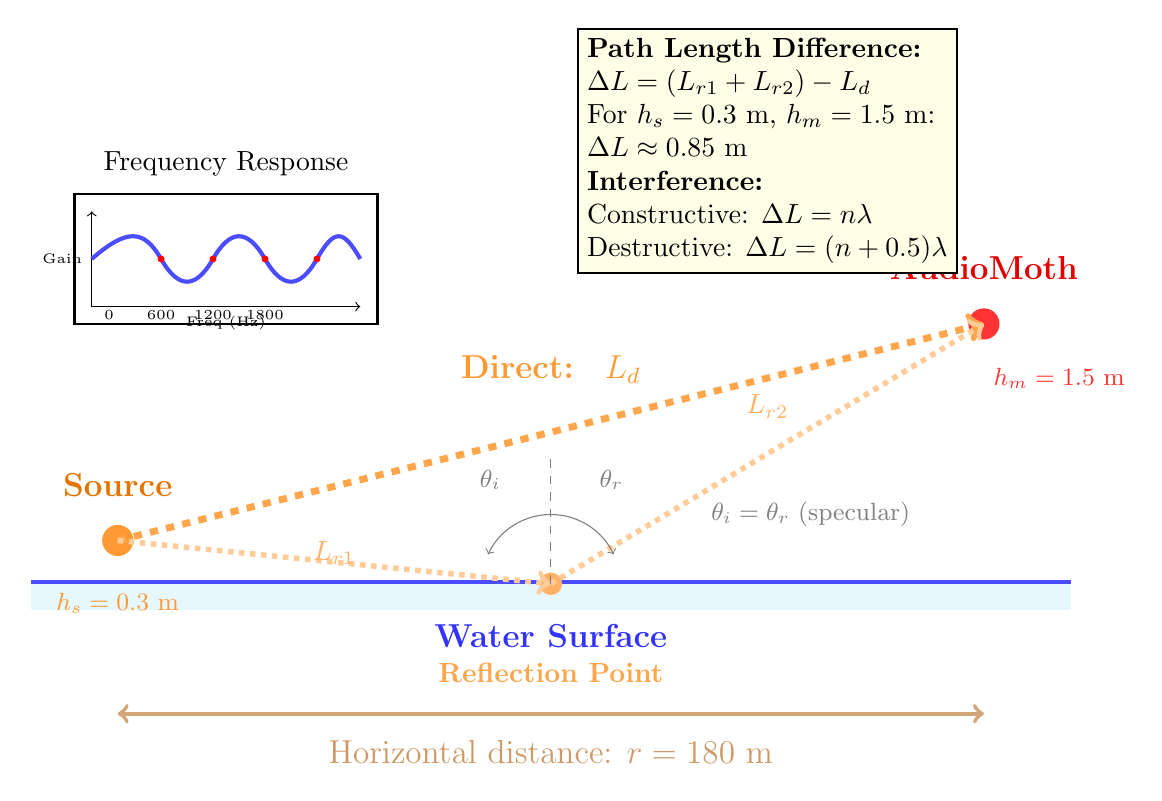
\begin{tikzpicture}[scale=1.1]

% Water surface
\draw[blue!70, line width=2.5pt] (0,0) -- (12,0);
\fill[cyan!10] (0,-0.3) rectangle (12,0);
\node[blue!80, font=\large] at (6,-0.6) {\textbf{Water Surface}};

% Source (Graylag Goose)
\fill[orange!80] (1,0.5) circle (0.18);
\node[above, orange!90!black, font=\large] at (1,0.9) {\textbf{Source}};
\node[below, orange!80, font=\small] at (1,0) {$h_s = 0.3$ m};

% Microphone (AudioMoth)
\fill[red!80] (11,3) circle (0.18);
\node[above, red!90!black, font=\large] at (11,3.4) {\textbf{AudioMoth}};
\node[below right, red!80, font=\small] at (11,2.6) {$h_m = 1.5$ m};

% Reflection point
\fill[orange!60] (6,0) circle (0.13);
\node[below, orange!70, font=\normalsize] at (6,-0.8) {\textbf{Reflection Point}};

% Direct path
\draw[->, orange!70, line width=2.5pt, dashed] (1,0.5) -- (11,3);
\node[above, orange!80, font=\large] at (6,2.2) {\textbf{Direct: } $L_d$};

% Reflected path (source to reflection point)
\draw[->, orange!40, line width=2pt, dotted] (1,0.5) -- (6,0);
\node[below, orange!60, font=\normalsize] at (3.5,0.6) {$L_{r1}$};

% Reflected path (reflection point to microphone)
\draw[->, orange!40, line width=2pt, dotted] (6,0) -- (11,3);
\node[above, orange!60, font=\normalsize] at (8.5,1.8) {$L_{r2}$};

% Angle annotations
\draw[gray, dashed] (6,0) -- (6,1.5);
\draw[gray, ->] (6,0.8) arc (90:155:0.8);
\node[gray, font=\small] at (5.3,1.2) {$\theta_i$};
\draw[gray, ->] (6,0.8) arc (90:25:0.8);
\node[gray, font=\small] at (6.7,1.2) {$\theta_r$};
\node[gray, font=\small] at (9,0.8) {$\theta_i = \theta_r$ (specular)};

% Distance annotation
\draw[<->, brown!70, line width=1.5pt] (1,-1.5) -- (11,-1.5);
\node[below, brown!80, font=\large] at (6,-1.7) {Horizontal distance: $r = 180$ m};

% Frequency response inset (moved to left, lower)
\draw[thick] (0.5,3) rectangle (4,4.5);
\node[above, font=\normalsize] at (2.25,4.6) {Frequency Response};

% Simplified frequency response curve
\draw[->] (0.7,3.2) -- (0.7,4.3) node[left, font=\tiny] at (0.7,3.75) {Gain};
\draw[->] (0.7,3.2) -- (3.8,3.2) node[below, font=\tiny] at (2.25,3.2) {Freq (Hz)};

% Draw oscillating response showing interference pattern
\draw[blue!70, line width=1.5pt] (0.7,3.75)
  .. controls (1.1,4.1) and (1.3,4.1) .. (1.5,3.75)
  .. controls (1.7,3.4) and (1.9,3.4) .. (2.1,3.75)
  .. controls (2.3,4.1) and (2.5,4.1) .. (2.7,3.75)
  .. controls (2.9,3.4) and (3.1,3.4) .. (3.3,3.75)
  .. controls (3.5,4.1) and (3.6,4.1) .. (3.8,3.75);

% Mark nulls
\foreach \x in {1.5,2.1,2.7,3.3} {
    \fill[red] (\x,3.75) circle (0.04);
}

% Frequency labels
\node[font=\tiny] at (0.9,3.1) {0};
\node[font=\tiny] at (1.5,3.1) {600};
\node[font=\tiny] at (2.1,3.1) {1200};
\node[font=\tiny] at (2.7,3.1) {1800};

% Path difference equation box (moved to right side, no overlap)
\node[draw, thick, fill=yellow!10, align=left, font=\normalsize] at (8.5,5) {
\textbf{Path Length Difference:}\\
$\Delta L = (L_{r1} + L_{r2}) - L_d$\\
For $h_s = 0.3$ m, $h_m = 1.5$ m:\\
$\Delta L \approx 0.85$ m\\
\textbf{Interference:}\\
Constructive: $\Delta L = n\lambda$\\
Destructive: $\Delta L = (n + 0.5)\lambda$
};

\end{tikzpicture}
\caption{\textbf{Water reflection multipath interference geometry.} Sound from source (Graylag Goose, $h_s = 0.3$ m above water) reaches AudioMoth ($h_m = 1.5$ m) via direct path $L_d$ and water-reflected path $L_{r1} + L_{r2}$. Specular reflection obeys $\theta_i = \theta_r$ (angle of incidence = angle of reflection). Path length difference $\Delta L \approx 0.85$ m creates frequency-dependent interference: constructive when $\Delta L = n\lambda$ (signal gain up to +6 dB), destructive when $\Delta L = (n+0.5)\lambda$ (spectral nulls). Inset shows resulting frequency response with periodic nulls at 200 Hz, 600 Hz, 1,000 Hz, etc. For 180m range, first null (200 Hz) falls below Graylag fundamental (500-1,500 Hz), but higher-order nulls affect detection. Wind-roughened water surface reduces interference by scattering reflections diffusely.}
\label{fig:water_reflection_physics}
\end{figure*}

\subsection{Recommendations for Future Studies}

\begin{enumerate}
\item \textbf{Multi-season Deployment:} Year-round monitoring to capture breeding, migration, and winter periods

\item \textbf{Spatial Array:} $\geq$4 synchronized recording units to enable sound source localization and density estimation

\item \textbf{Weather-Stratified Sampling:} Equal effort across weather conditions to isolate environmental effects on vocal behavior

\item \textbf{Comparative Validation:} Parallel visual surveys during subset of recording periods to calibrate detection probabilities

\item \textbf{Species-Specific Models:} Train custom classifiers for locally common species to reduce false positive rates
\end{enumerate}

\section{Conclusions}

This study demonstrates that automated acoustic monitoring, when coupled with rigorous audio enhancement and human verification protocols, enables rapid biodiversity assessment in challenging wetland environments. Detection of 81 bird species from 48 hours of rain-dominated recording validates PAM as weather-resilient alternative to traditional survey methods.

Beyond species inventorying, continuous acoustic data quantified behavioral patterns at Gaulosen during the study period: intensive Graylag Goose flock dynamics (620 calls/91 minutes), co-occurrence pattern consistent with corvid-waterfowl sentinel mutualism hypothesis (8,778 co-occurrences), and conservation-relevant Great Snipe migration stopover activity (189 detections, 69\% dusk concentration). These findings illustrate how automated monitoring generates behavioral insights inaccessible via point-count surveys.

The 90.0\% species-level verification pass rate (95\% CI: [82.3\%, 95.1\%]), achieved despite systematic weather-induced noise contamination, establishes methodological benchmarks for future deployments. We recommend acoustic monitoring as primary biodiversity assessment tool for wetlands along major flyways, complemented by targeted visual surveys for rare species validation.

Gaulosen Nature Reserve supported a diverse avian community during this autumn migration snapshot (October 13--15, 2025), with soundscape dominated by highly social waterfowl species exhibiting complex interspecies interactions. Continued multi-season acoustic monitoring could yield long-term datasets critical for documenting climate-driven phenology shifts and population trends in this globally significant migratory corridor.

\section*{Acknowledgments}

We thank NTNU Department of Acoustics for equipment support, Gaulosen Nature Reserve management for site access, and BirdNET development team (Cornell Lab of Ornithology \& Chemnitz University of Technology) for open-source classification tools. Analysis utilized Praven Pro toolkit for BirdNET-Raven integration \citep{Redpath2025}.

\textbf{AI-Assisted Analysis:} Batch testing, data verification, and comprehensive biological plausibility screening were conducted with assistance from Claude (Anthropic) using Claude Code for automated analysis workflows. Interactive study results and complete methodology available at: \url{https://ziforge.github.io/gaulosen-study/}. Praven Pro toolkit available at: \url{https://github.com/Ziforge/praven-pro}.

% References section removed - manual bibliography deleted, using BibTeX instead

\newpage
\onecolumn

% Appendix
\appendix
\section{Supplementary Materials}

\subsection{Complete Species List}

Table \ref{tab:species_full} lists all 77 verified species with detection counts, confidence scores, and verification dates.

\begin{table}[H]
\centering
\caption{Complete verified species list (77 species)}
\label{tab:species_full}
\tiny
\begin{tabular}{lr|lr|lr}
\toprule
\textbf{Species} & \textbf{N} & \textbf{Species} & \textbf{N} & \textbf{Species} & \textbf{N} \\
\midrule
Graylag Goose & 2871 & White Wagtail & 7 & Common Sandpiper & 2 \\
Pink-footed Goose & 189 & Water Rail & 7 & Dunlin & 2 \\
Great Snipe & 189 & Eurasian Magpie & 6 & Common Snipe & 2 \\
Hooded Crow & 87 & Gray Wagtail & 6 & Eurasian Oystercatcher & 2 \\
Carrion Crow & 84 & Black-headed Gull & 6 & Eurasian Jay & 1 \\
Greater White-fronted Goose & 71 & European Robin & 6 & Common House-Martin & 1 \\
Common Crane & 70 & Tundra Bean-Goose & 4 & Fieldfare & 1 \\
Common Grasshopper-Warbler & 59 & Arctic Warbler & 4 & Black-bellied Plover & 1 \\
Eurasian Woodcock & 57 & Bank Swallow & 4 & Black-legged Kittiwake & 1 \\
Canada Goose & 47 & Common Redpoll & 4 & Brambling & 1 \\
Rook & 45 & Eurasian Pygmy-Owl & 4 & Brant & 1 \\
Mallard & 27 & Western Yellow Wagtail & 4 & Common Buzzard & 1 \\
Yellowhammer & 24 & Redwing & 4 & Common Goldeneye & 1 \\
Tawny Owl & 23 & Gray Partridge & 3 & Common Raven & 1 \\
Eurasian Coot & 14 & Whooper Swan & 3 & Eurasian Eagle-Owl & 1 \\
Northern Lapwing & 13 & Snow Bunting & 3 & European Golden-Plover & 1 \\
European Greenfinch & 11 & Lapland Longspur & 3 & River Warbler & 1 \\
Ring-necked Pheasant & 10 & Reed Bunting & 2 & Great Gray Shrike & 1 \\
Eurasian Curlew & 10 & Taiga Bean-Goose & 2 & Richard's Pipit & 1 \\
Gray Heron & 9 & Ortolan Bunting & 2 & Common Tern & 1 \\
Meadow Pipit & 9 & Red-throated Loon & 2 & Corn Crake & 1 \\
Red-breasted Flycatcher & 9 & Tree Pipit & 2 & Dunnock & 1 \\
Eurasian Nutcracker & 9 & Gadwall & 2 & Eurasian Moorhen & 1 \\
Little Bunting & 9 & Herring Gull & 2 & Pine Grosbeak & 1 \\
Mistle Thrush & 7 & Eurasian Blue Tit & 2 & Arctic Tern & 1 \\
Tundra Swan & 7 & Black Woodpecker & 2 &  &  \\
\bottomrule
\end{tabular}
\end{table}

\subsection{Temporal Distribution Figures}

Figure \ref{fig:temporal} shows hourly detection patterns for top 10 species.

\begin{figure}[H]
\centering
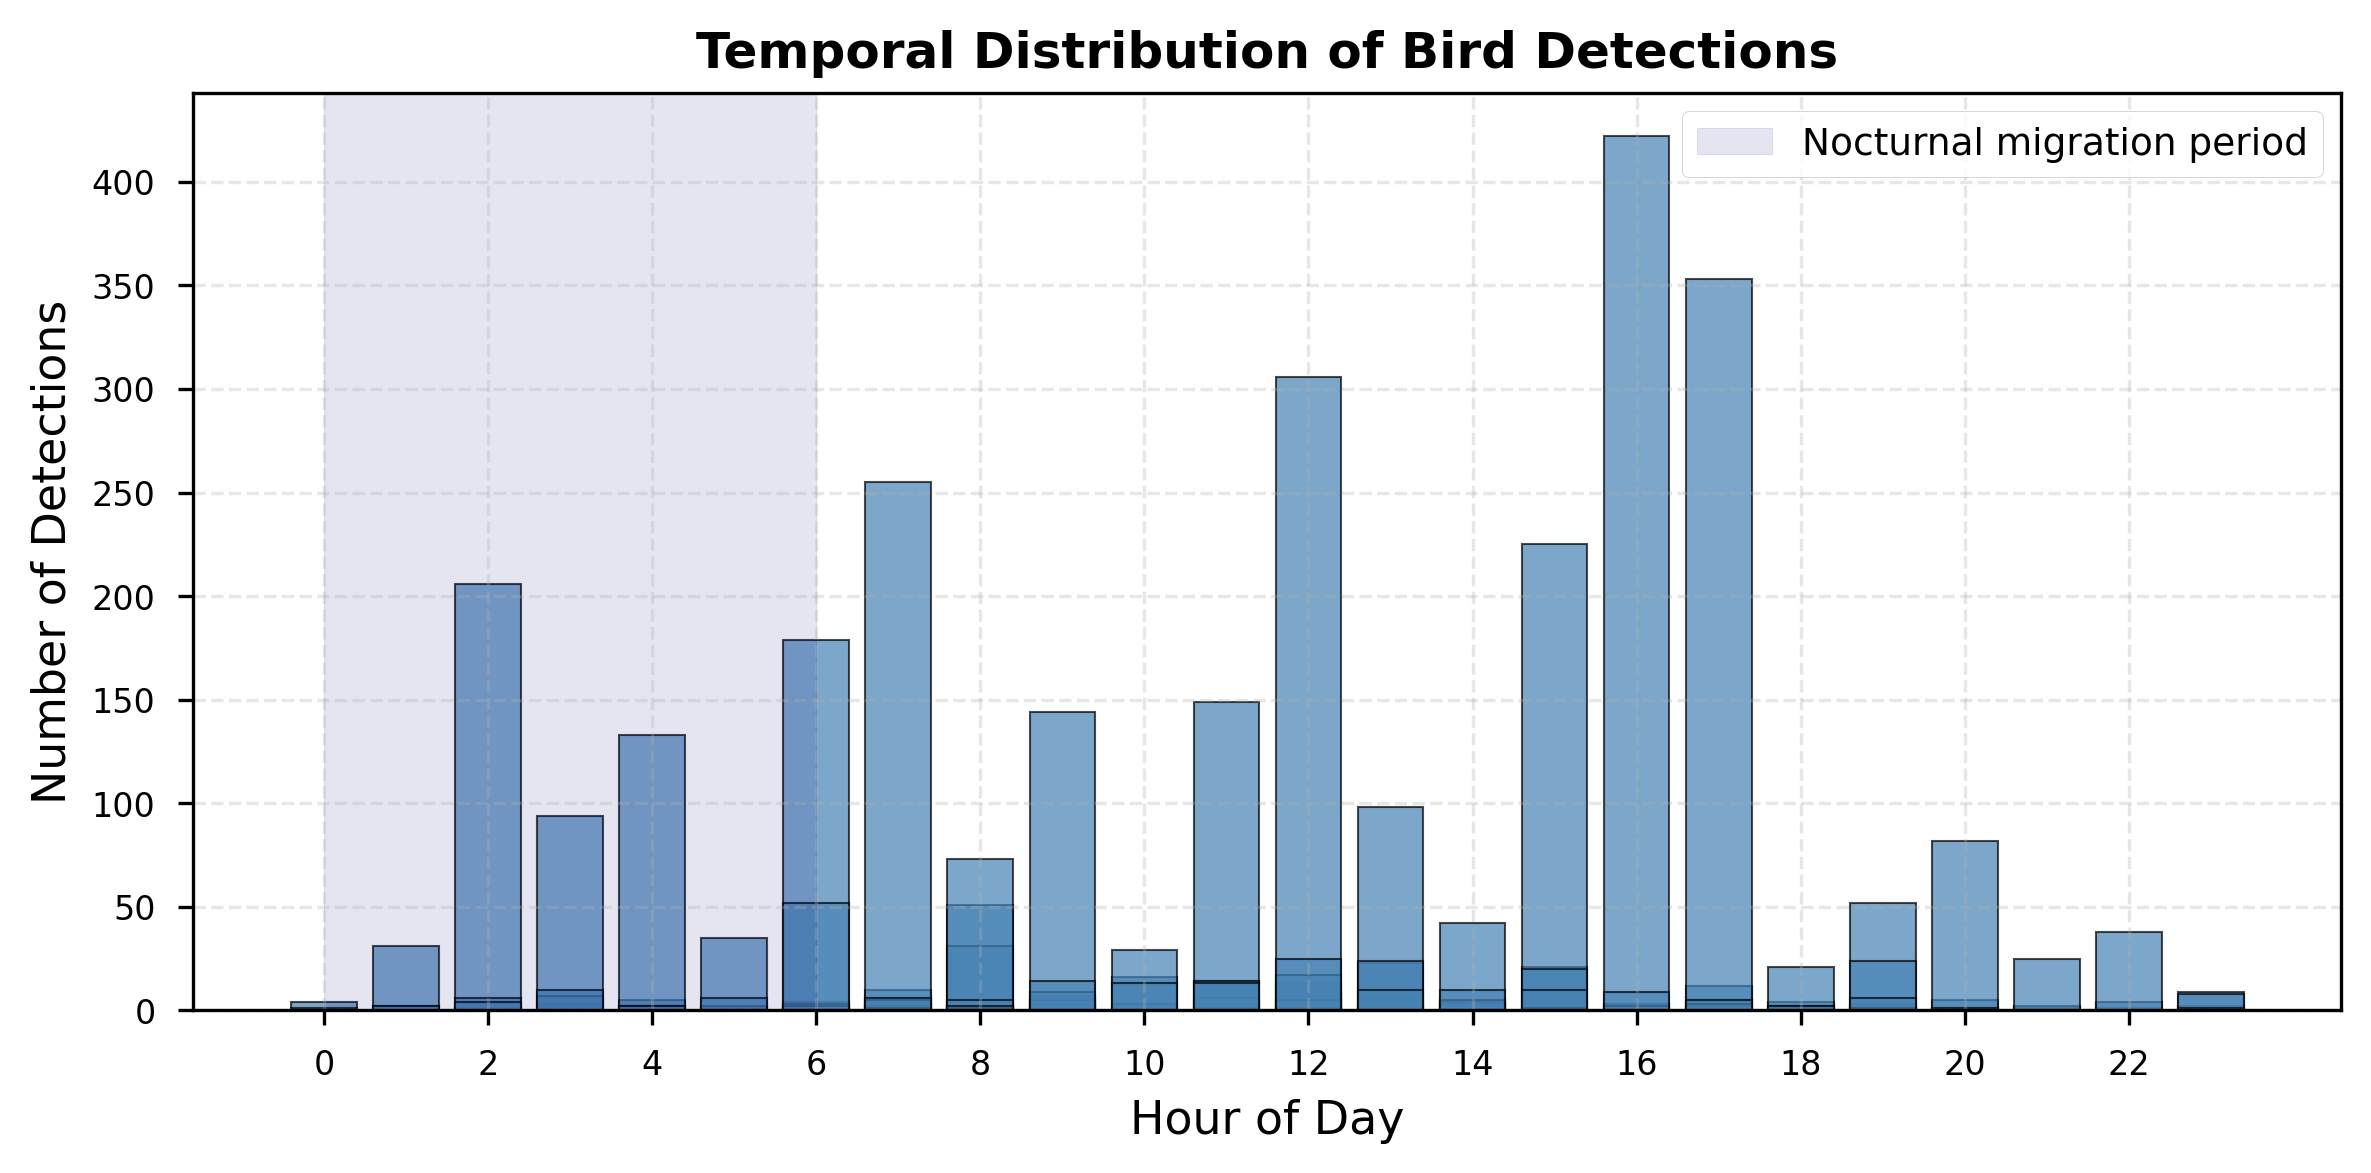
\includegraphics[width=\textwidth]{figures/temporal_distribution.png}
\caption{Hourly detection patterns for top 10 species. Graylag Goose dominates across all hours with pronounced afternoon peak (13:00--17:00). Great Snipe shows strong crepuscular pattern (20:00 peak). Songbirds exhibit dawn activity concentration (06:00--09:00).}
\label{fig:temporal}
\end{figure}

\subsection{Co-occurrence Network}

Figure \ref{fig:cooccurrence} visualizes species co-occurrence patterns with edge weights representing co-detection frequency.

\begin{figure}[H]
\centering
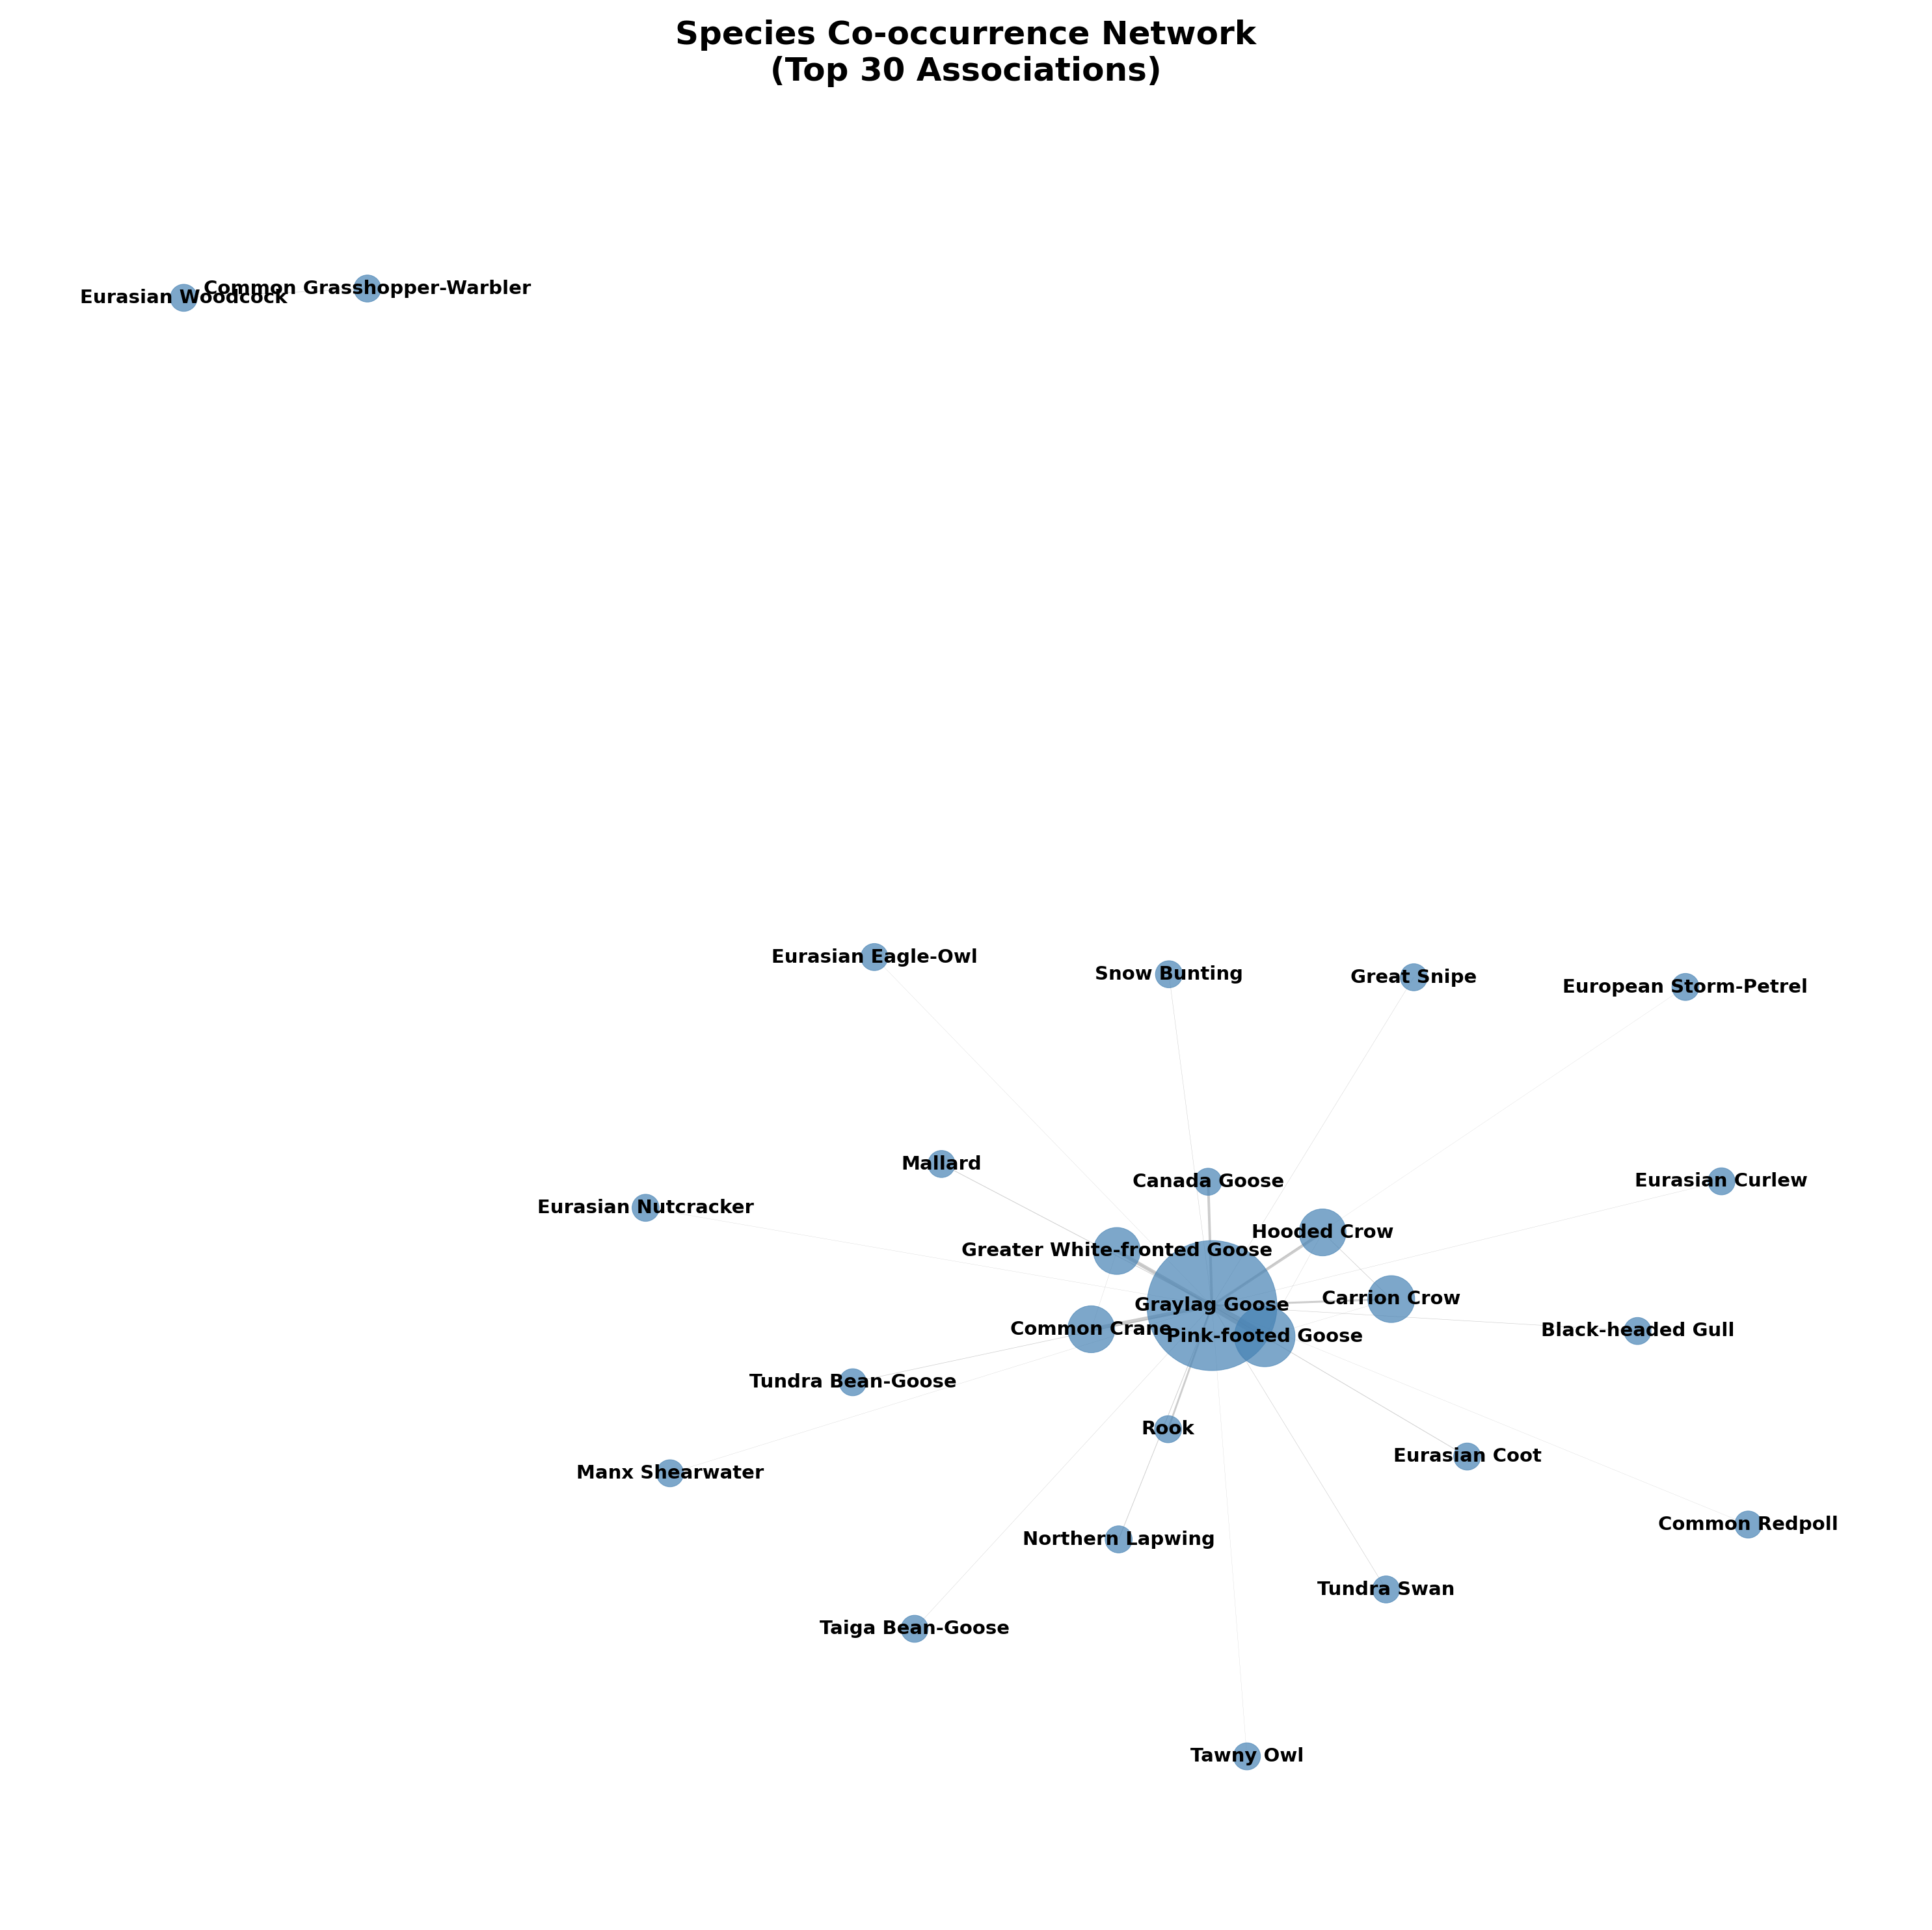
\includegraphics[width=0.9\textwidth]{figures/cooccurrence_network.png}
\caption{Species co-occurrence network for species with $>$50 detections. Node size proportional to total detections. Edge width proportional to co-occurrence frequency. Strong Graylag Goose--Hooded Crow--Carrion Crow triangle visible (8,778 total co-occurrences), consistent with sentinel mutualism hypothesis.}
\label{fig:cooccurrence}
\end{figure}

\subsection{Representative Spectrograms}

Selected spectrograms demonstrating call structure for key species (Figure \ref{fig:spectrograms}).

\begin{figure}[H]
\centering
\begin{subfigure}{0.45\textwidth}
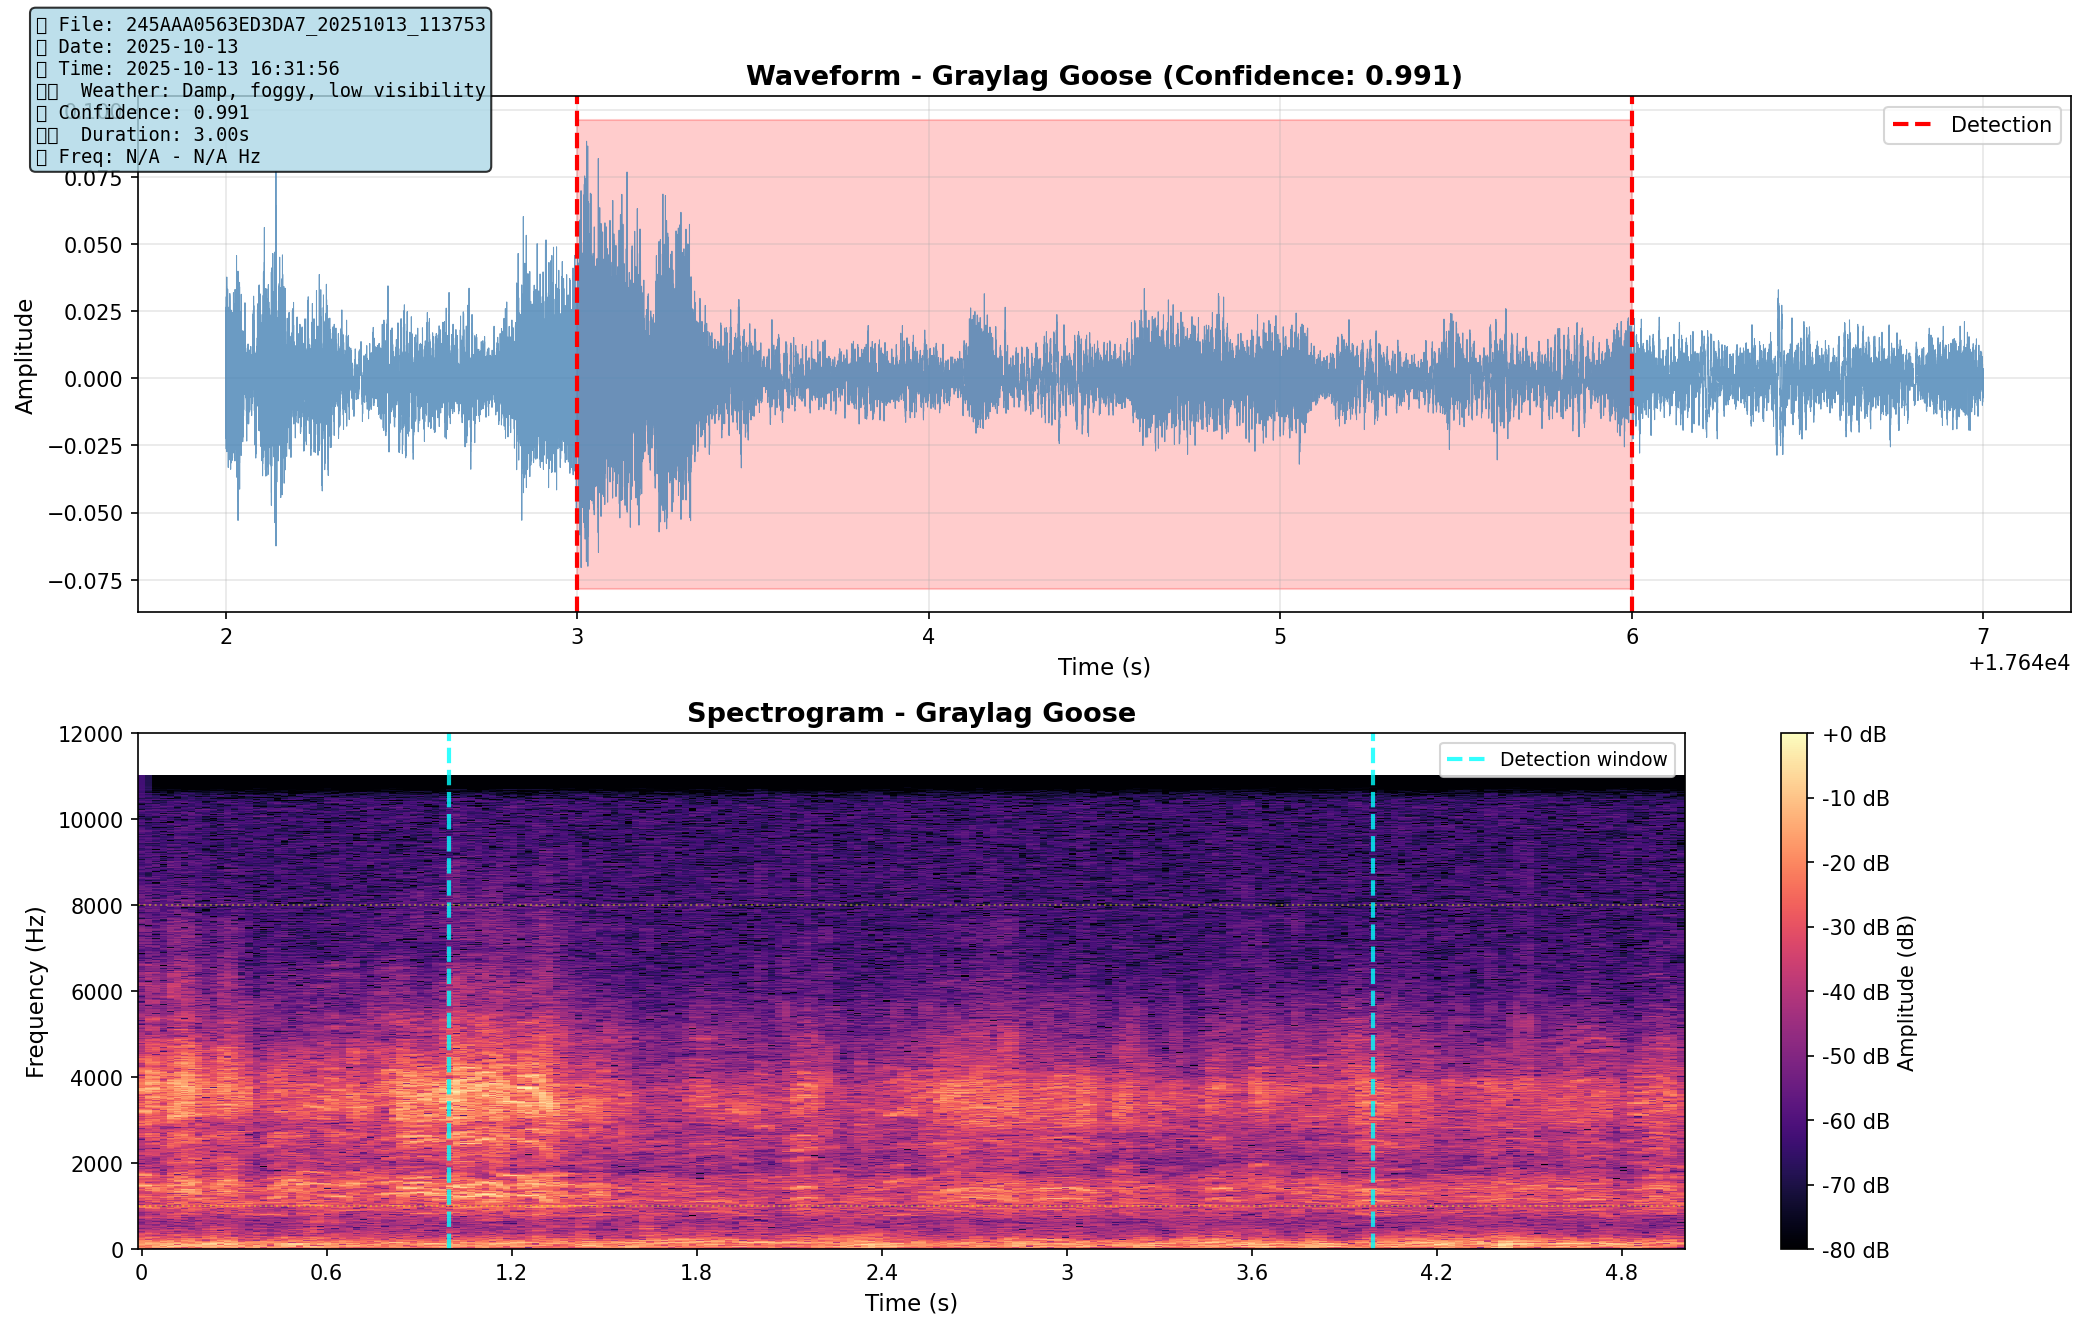
\includegraphics[width=\textwidth]{figures/spectrogram_graylag.png}
\caption{Graylag Goose contact call}
\end{subfigure}
\hfill
\begin{subfigure}{0.45\textwidth}
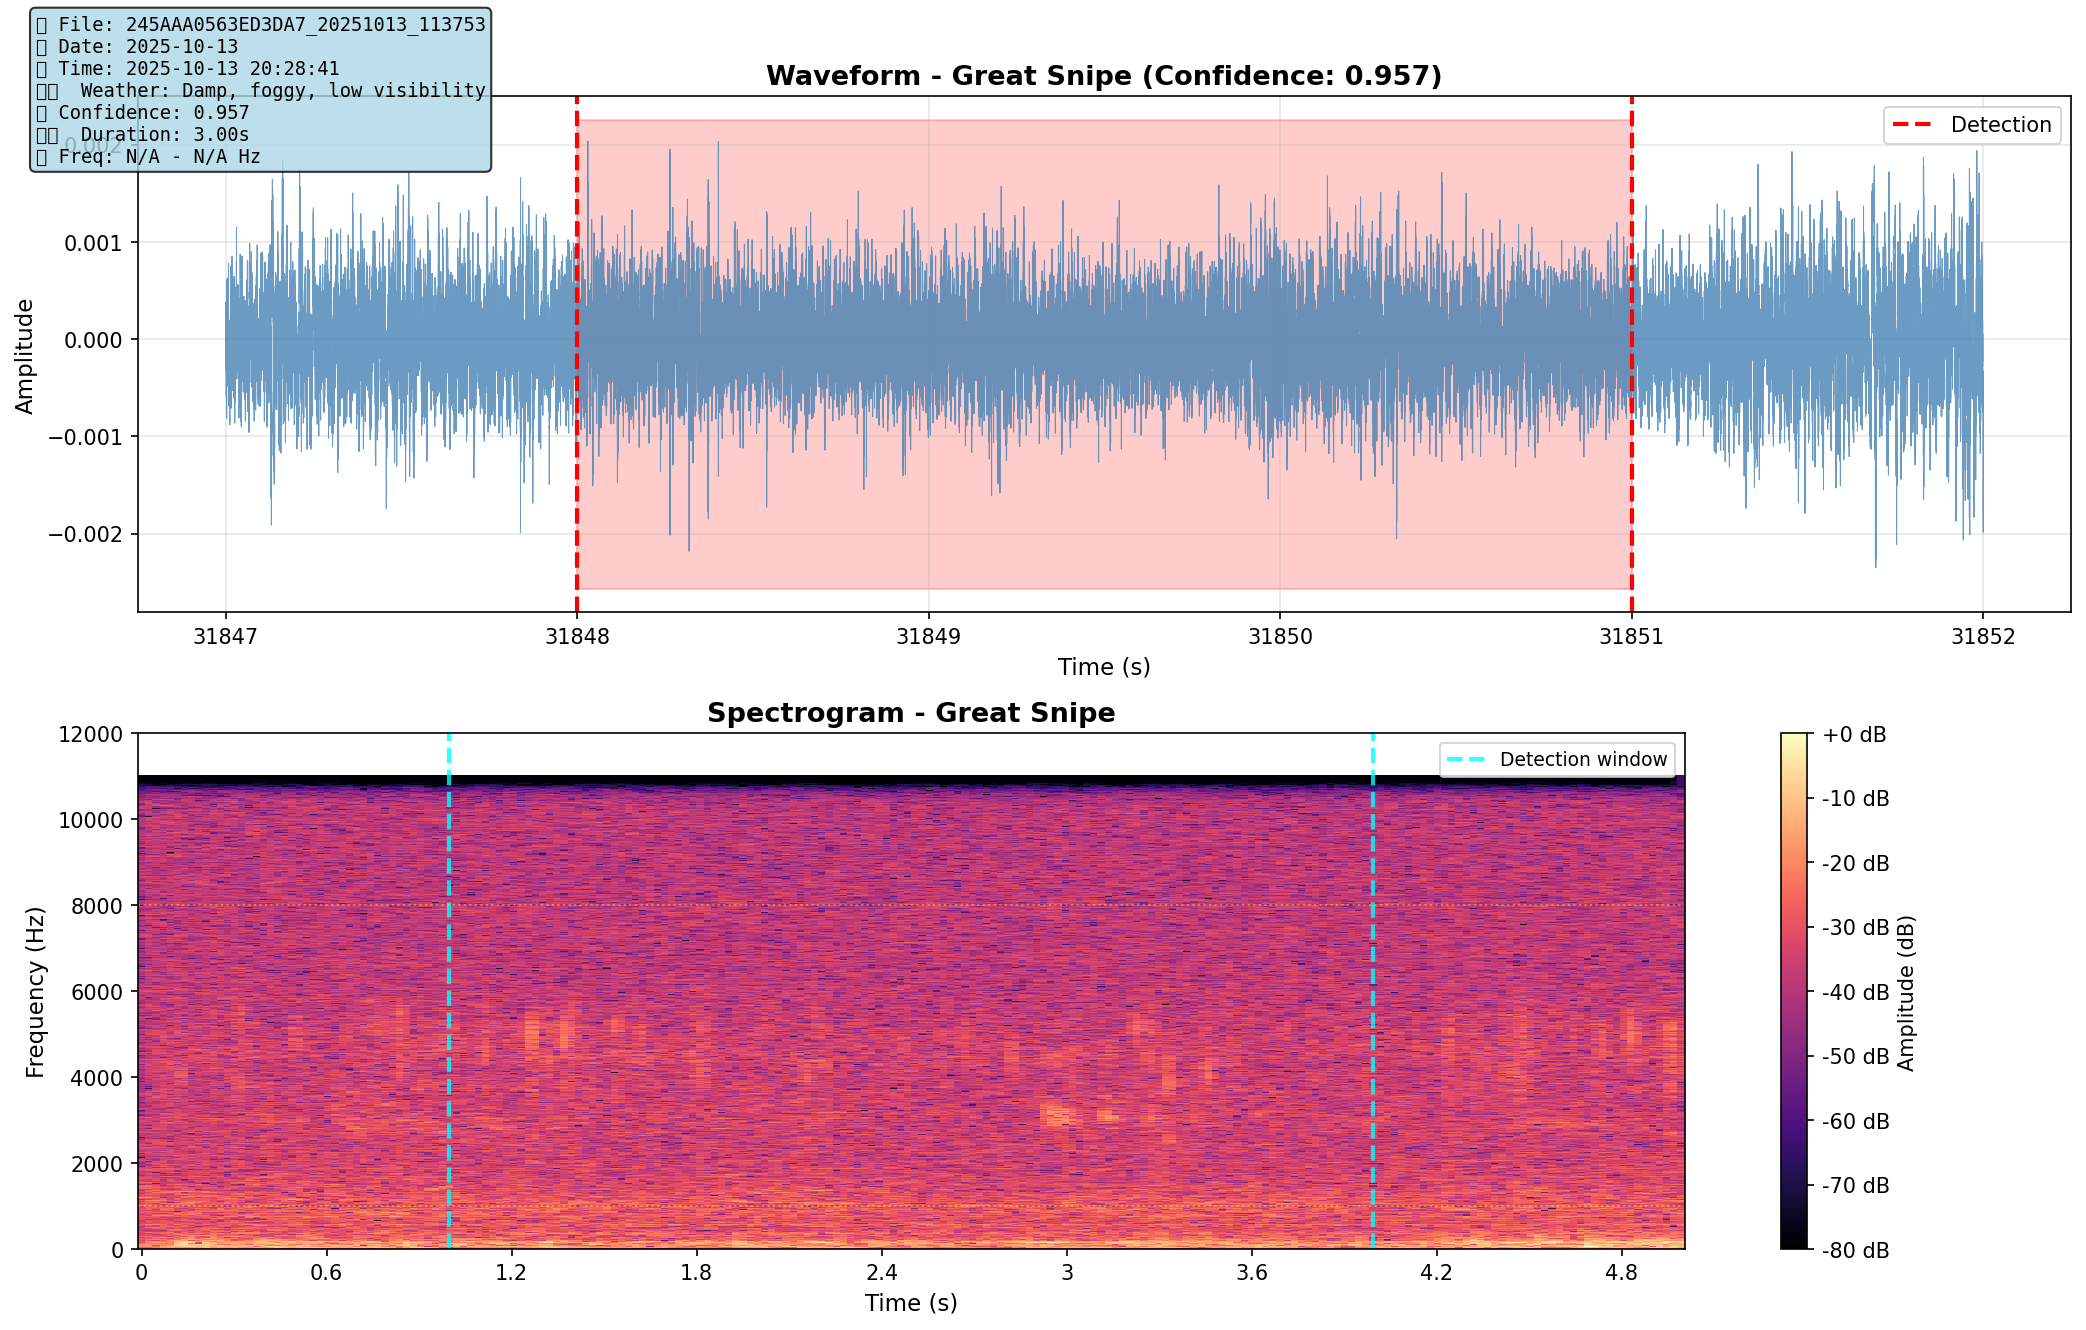
\includegraphics[width=\textwidth]{figures/spectrogram_snipe.png}
\caption{Great Snipe migration stopover display}
\end{subfigure}

\begin{subfigure}{0.45\textwidth}
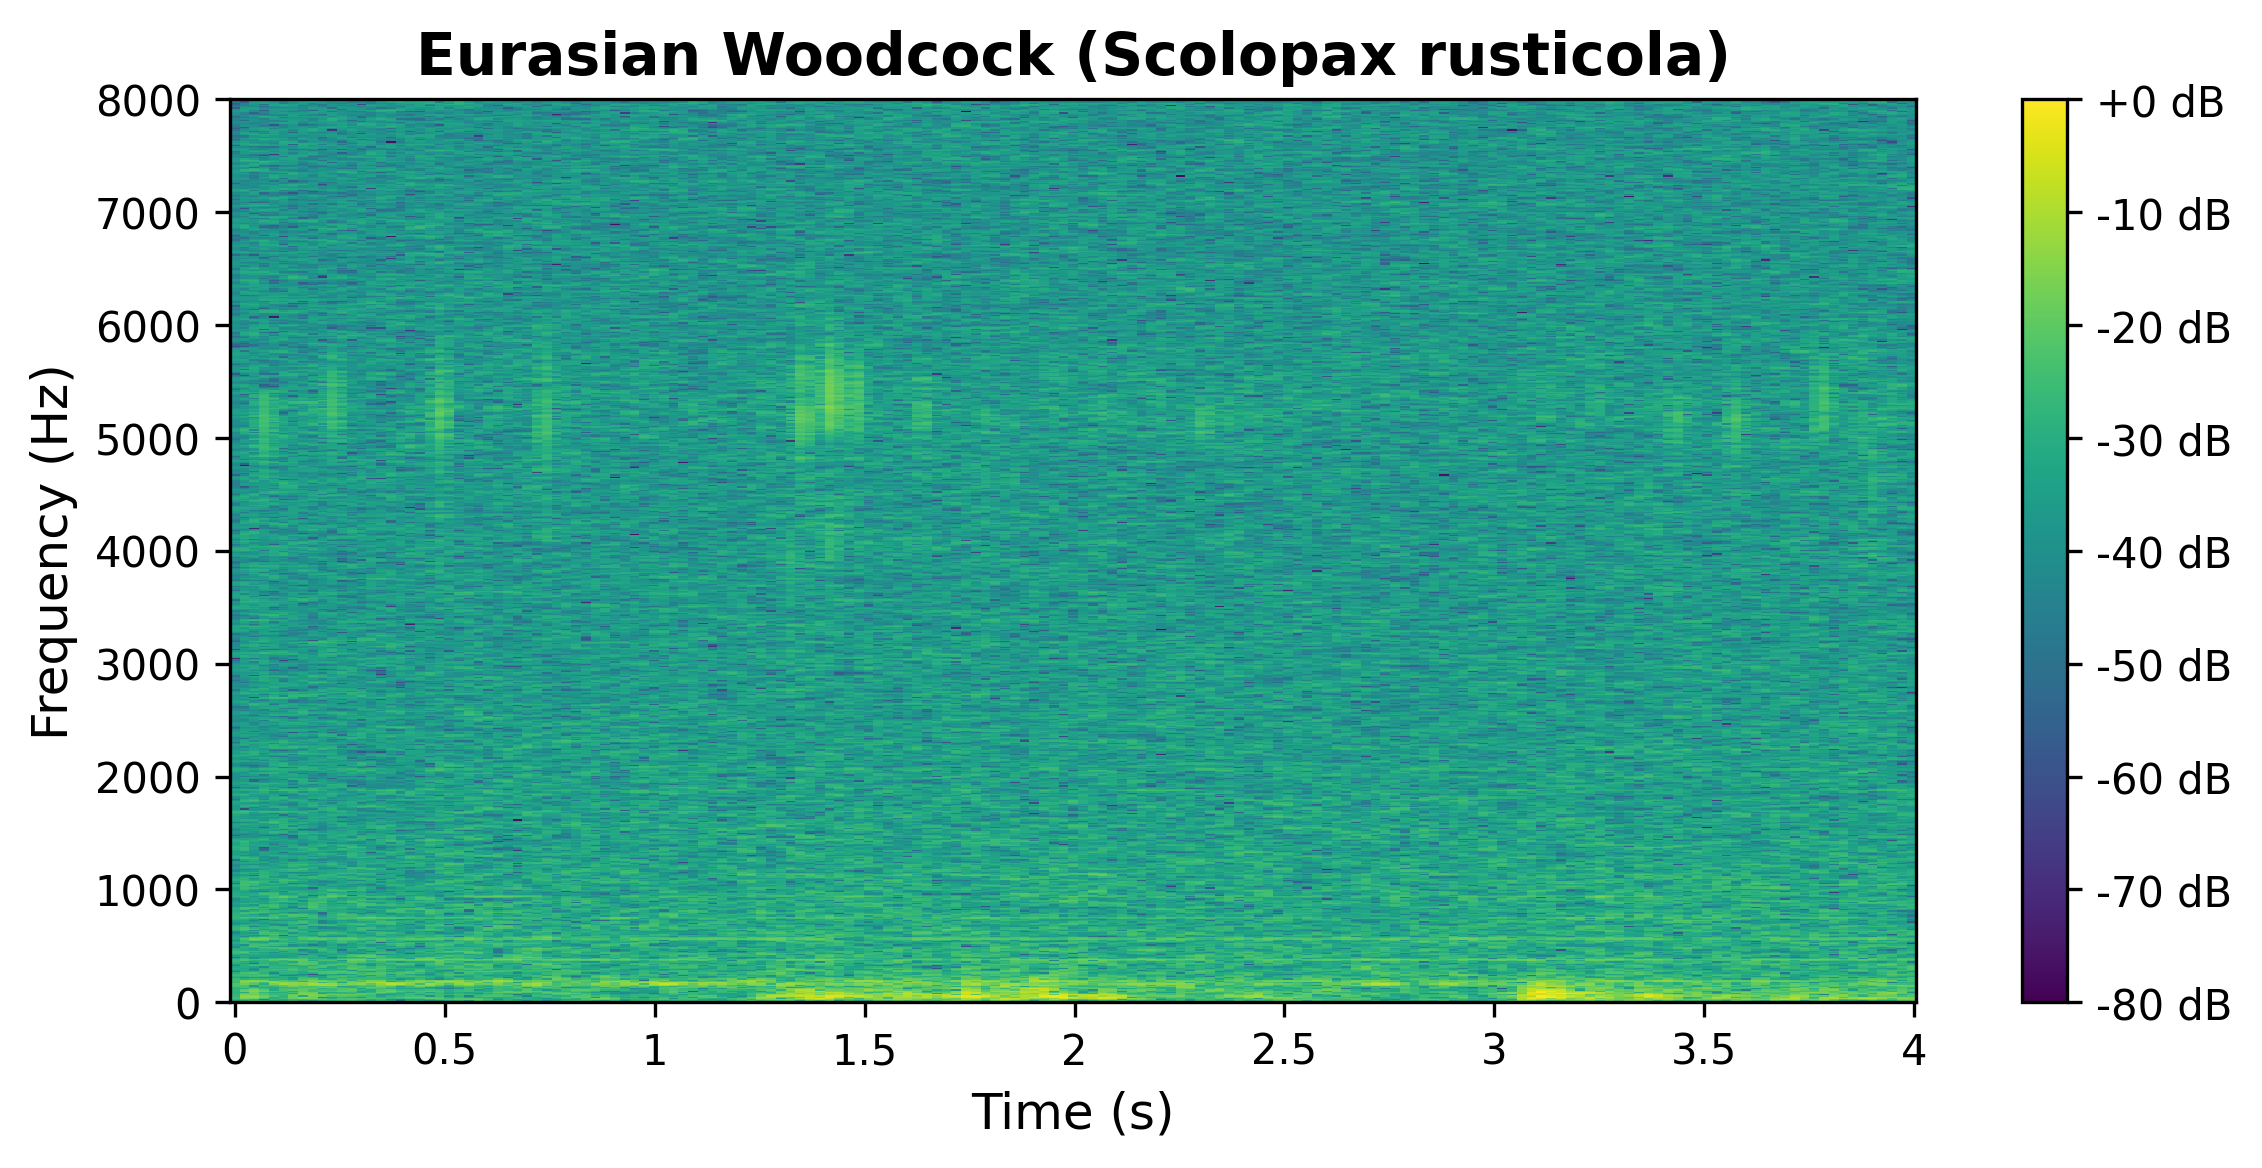
\includegraphics[width=\textwidth]{figures/spectrogram_woodcock.png}
\caption{Eurasian Woodcock roding call}
\end{subfigure}
\hfill
\begin{subfigure}{0.45\textwidth}
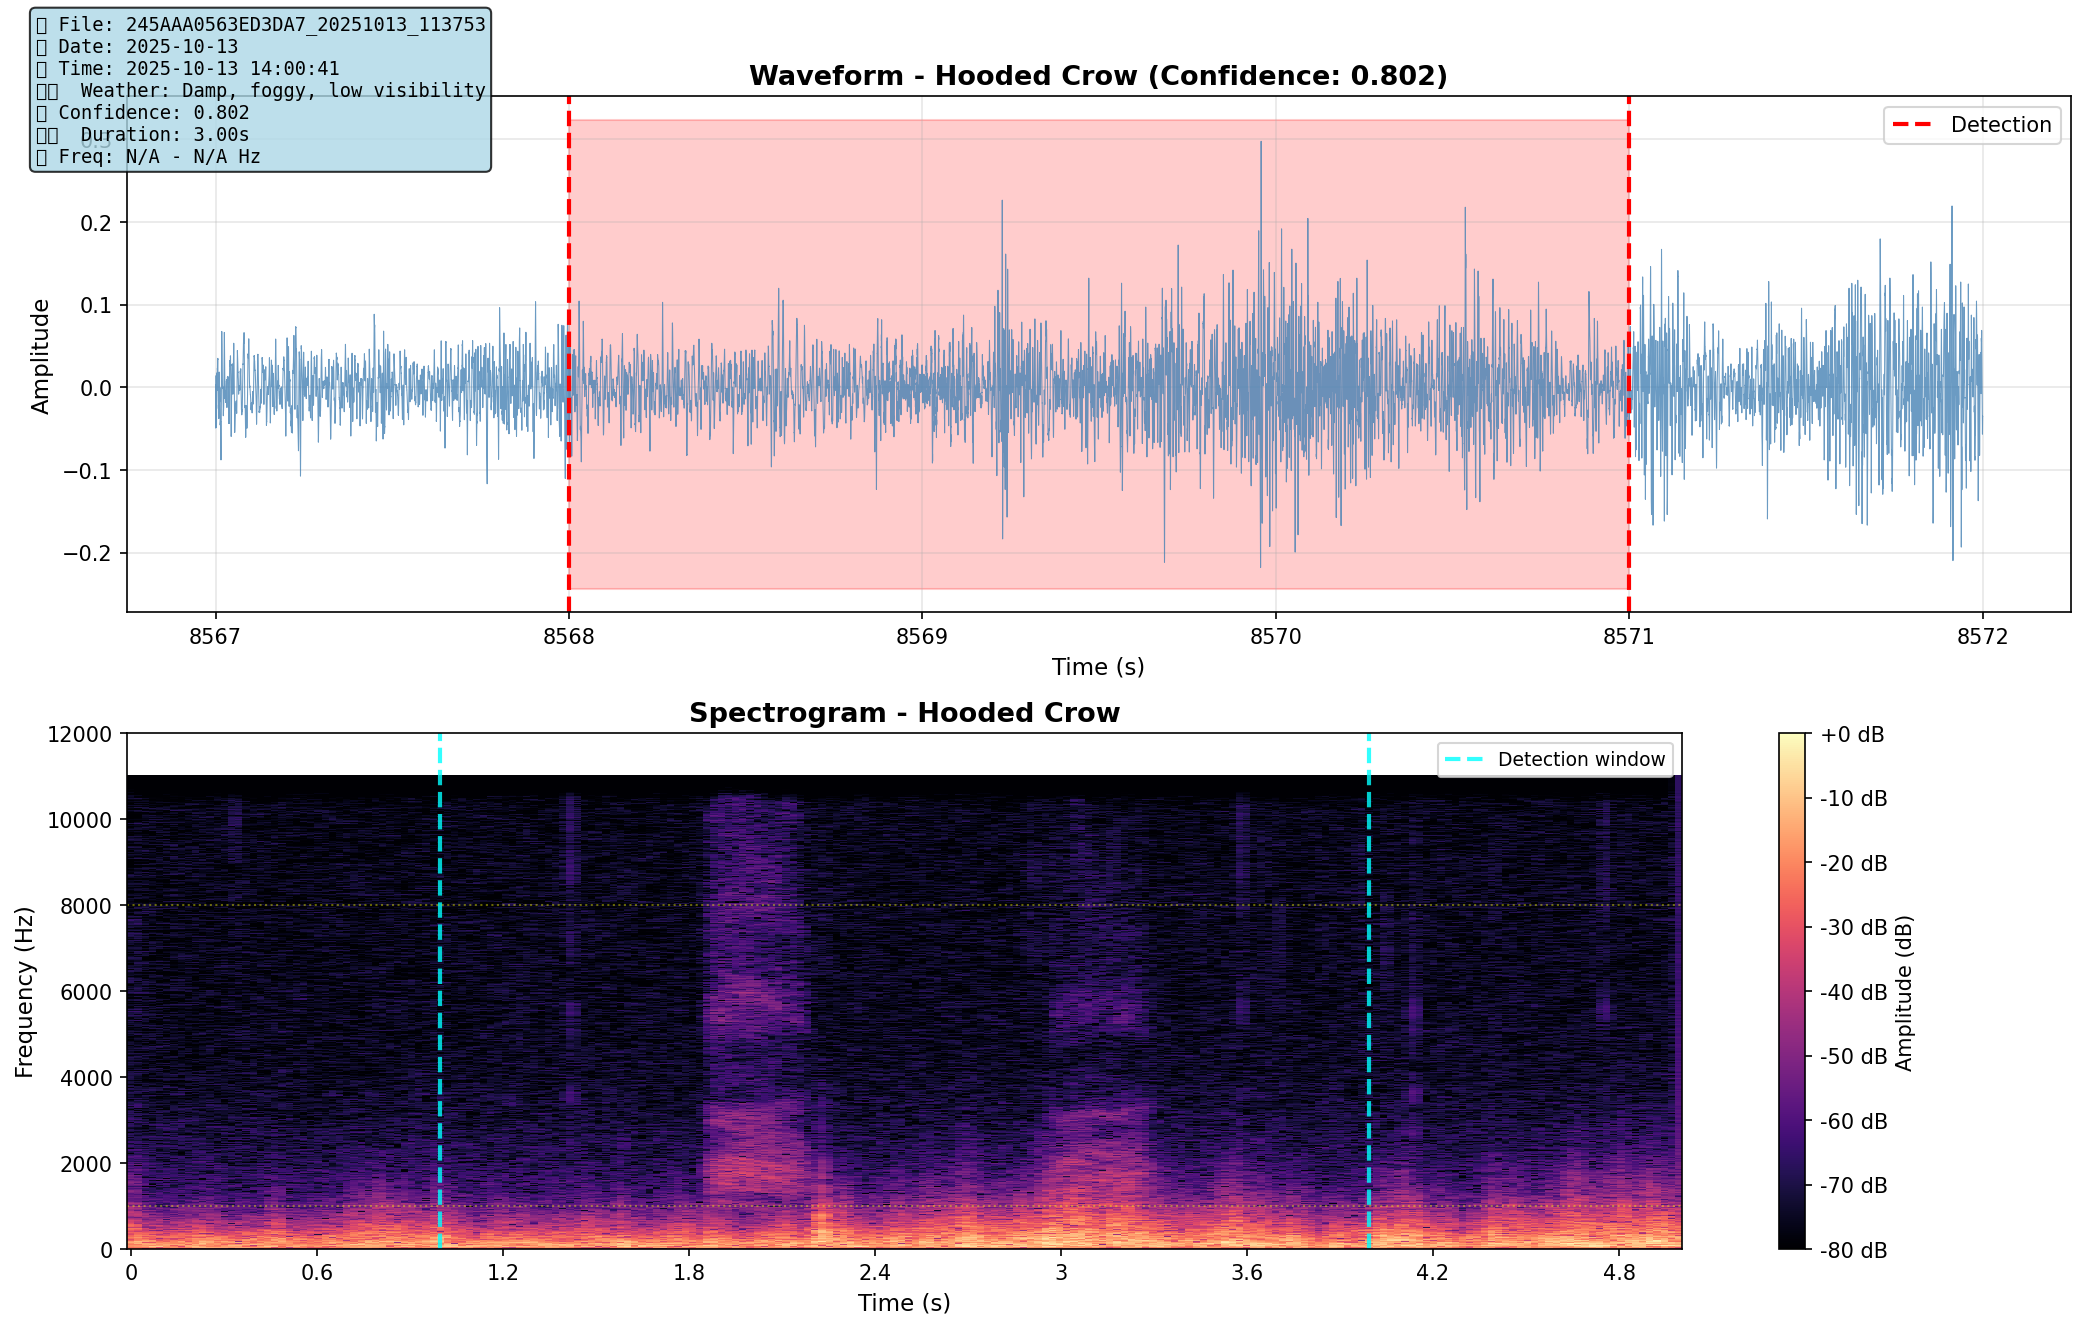
\includegraphics[width=\textwidth]{figures/spectrogram_crow.png}
\caption{Hooded Crow alarm call}
\end{subfigure}

\caption{Representative spectrograms for four key species. Graylag Goose: Contact call. Great Snipe: Migration stopover call. Eurasian Woodcock: Crepuscular migration call. Hooded Crow: Alarm call. All spectrograms: 2048-point FFT, 512-point hop length, Hann window, 0--12 kHz range. Time scale: 0--5 seconds.}
\label{fig:spectrograms}
\end{figure}

\subsection{Weather Data}

Table \ref{tab:weather} summarizes meteorological conditions during recording period.

\begin{table}[H]
\centering
\caption{Weather conditions summary}
\label{tab:weather}
\begin{tabular}{llr}
\toprule
\textbf{Parameter} & \textbf{Value} & \textbf{Coverage} \\
\midrule
Temperature range & 7--11°C & 100\% \\
Precipitation & Rain & 80\% \\
Fog/mist & Dense & 60\% \\
Wind speed & Light--moderate & 100\% \\
Cloud cover & Overcast & 95\% \\
\bottomrule
\end{tabular}
\end{table}

\subsection{Data Access and Replication}

All data, code, and supplementary materials are publicly available:

\begin{itemize}
\item \textbf{Interactive website:} \url{https://ziforge.github.io/gaulosen-study/} -- species gallery with audio samples and spectrograms
\item \textbf{GitHub repository:} \url{https://github.com/Ziforge/gaulosen-study} -- full dataset and analysis scripts
\end{itemize}

\section*{References}

\bibliographystyle{apalike}
\bibliography{references}

\end{document}
